\documentclass{article}
\usepackage[top=1in,bottom=1in,left=1in,right=1in]{geometry}
\usepackage{inputenc}
%\usepackage{ctex}
%\usepackage{natbib}
\usepackage{graphicx}
\usepackage{caption}
\usepackage{subfigure}
\usepackage{amsmath}
\usepackage{amsfonts}
\usepackage{xeCJK}
\usepackage{float}
\usepackage{subfig}

\usepackage{algorithm}  
\usepackage{algorithmicx}  
\usepackage{algpseudocode}  
\usepackage{amsmath}  

\usepackage{setspace}

\floatname{algorithm}{算法}  
\renewcommand{\algorithmicrequire}{\textbf{输入:}}  
\renewcommand{\algorithmicensure}{\textbf{输出:}} 


\newcommand{\tabincell}[2]{
\begin{tabular}{@{}#1@{}}#2\end{tabular}
}

%\usepackage{cite}
\setCJKmainfont{STSong}
\graphicspath{ {./graph/} }
\renewcommand{\figurename}{图}
\renewcommand{\tablename}{表}
\renewcommand\refname{参考文献}

\renewcommand{\baselinestretch}{2.0}

\title{基于排队网络的共享单车坏车运维建模与优化}


\begin{document}

% \maketitle

\textbf{Abstract}
The operation and maintenance of the broken car in the shared bicycle system mainly includes three processes: recollecting, repairing and releaseing. This paper considers the operating characteristics of batch recycling, centralized maintenance and batch delivery of shared bicycles, constructs a queuing network model, and calculate the system performance parameters through the state transition equation and simulation of the Markov process to study the system. Then determine the allocation of resources in the system between the maintenance center and the recovery and release of vehicles, under the constraint of limited total resources. In view of the limited and discrete features of the solution space, we adopt a Ranking and Selection algorithm, to chose the optimal or near optimal setting with the goal of minimizing the loss rate of customers. We have found that increasing the operating speed or number of maintenance and delivery vehicles can improve system performance, but there is a marginal diminishing effect. When the overall operating capacity of the system is limited, adding trucks can more effectively improve system performance. When the gap between maintenance and delivery capabilities is small, the system's service capabilities are stronger. At last, we demonstrate the validation that algorithm adopted in this paper can effectively select a good system arrangement. \\

% %\newpage
% %\textbf{摘要}
% 共享单车系统中坏车的运维主要包括回收、维修和投放三个过程。本文重点研究这三个过程对共享单车系统整体服务能力的影响。通过将共享单车的使用和运维建模成排队网络,给出系统长程状态下的状态概率方程组。求解该方程组获得系统的稳定状态概率。进一步通过系统状态概率计算,给出系统的运行特征计算公式,如系统中可以使用的车辆数占总体的比例、丢失的顾客比例等。最后在设置的算例上进行数值实验,分析运维环节的能力变化对系统整体状态的影响。实验结果显示,当系统整体运行能力有限时,需要匹配回收和投放的能力,二者相近时,系统服务能力较强。而回收批量和投放批量应当尽可能小。提升系统中单一环节的运维能力对单车系统整体的运维状态影响存在边际递减的现象。
% \textbf{摘要}
% 共享单车系统中坏车的运维主要包括回收、维修和投放三个过程。其中如何分配维修能力和运载能力仍待解决。本文在运维总能力有限的约束下,考虑共享单车批量回收、集中维修和批量投放的运行特点,构建排队网络模型,通过马尔可夫过程的状态转移方程和仿真求解系统性能参数,以研究系统运维安排对系统性能表现的影响。进一步在系统中资源有限情况下,求解维修能力和运载能力之间的最优分配。针对解空间有限、离散的特征,结合Ranking and Selection算法,以最小化服务顾客的损失率为目标进行决策。研究发现,提升维修和运载车的运行速率或数量均可以改善系统性能表现,但存在边际递减效应。当系统整体运行能力有限时,增加运载车能更有效地改善系统表现。维修和运载的能力差距不大时,系统服务能力较强。本文采用的算法可以有效地选择出最优或接近最优的系统安排。

\textbf{摘要}
运行过程中不断产生的坏车是当前共享单车运营面临的一个重要问题。研究针对坏车进行的回收、维修和投放过程怎样影响系统、如何解决相应的决策问题具有重要意义。本文考虑共享单车批量回收、集中维修和批量投放的运行特点,构建封闭排队网络模型,基于连续时间马尔可夫过程的长程稳态和蒙特卡洛仿真方法分析共享单车系统的运维过程对系统性能表现的影响。进一步,在可分配资源有限的约束下,决策维修能力和对应回收和投放的运载能力之间的最优配置。针对解空间有限、离散的特征,结合Ranking and Selection算法,以最小化服务顾客的损失率为目标进行决策。研究发现,提升维修和运载车的运行速率或数量均可以改善系统性能表现,但存在边际递减效应。当系统整体运行能力有限时,增加运载车能更有效地改善系统表现。本文所采用的算法可以有效地选择出最优或接近最优的系统设置。

\newpage

\section{引言}
% 随处可见的共享单车已成为人们日常通勤的重要方式。但最初并非现在这样的模式,而是许多城市的有桩公共自行车。借助移动互联网的浪潮,共享单车迅速遍布中国,颠覆了传统的固定车桩的模式。同样也是由于互联网浪潮,前期积累用户基数的商业模式,让过量的单车投放一度成为一个社会治理问题。随着政策的出台和行业竞争程度的逐渐降低,共享自行车行业迈过初期野蛮生长阶段,进入了几家分庭抗礼的状态。当前单车系统的运维成为了各运营商更加关注的问题。根据企鹅智库2018年发布的《共享单车数据报告:解读摩拜ofo们的用户与未来》中显示,ofo用户对于共享单车的不满体验中,想骑的时候没有车子的比例高达55.2\%、往返需求难以同时满足的比例是41.4\%。并且单车中上报车辆故障的比例为39.3\%。单车的损坏不仅影响用户体验;对单车的运营公司而言,损坏的车更增加了回收、维修和重新投放的成本,直接导致收入的损失以及品牌声誉的下降。在共享单车的使用场景中,不能被及时满足的顾客骑行需求,会迅速被其他方式所替代,比如乘客可能选择步行或打车。于是,在单车的运营中好车的调度和坏车的回收、维修和重新投放对整个共享单车系统的高效运行有着决定性意义。对好车(正在各个区域正常服务的共享单车,后文同)的调度而目前已有大量研究,而对坏车(不能服务顾客的共享单车,包括已维修但未投放运营的单车,后文同)的回收、维修和投放的研究工作还很少。本文通过对共享单车运维系统建立封闭排队网络模型,探究了单车运营各个环节对系统整体服务性能的影响。进一步,结合排选算法,在资源约束的条件下,求解系统最佳的运维安排。

共享单车因其便捷性,已成为人们日常通勤的重要方式。根据交通运输部公布的数据,截至2019年8月底,我国互联网租赁自行车共有1950万辆,覆盖全国360个城市,注册用户数超过3亿人次,日均订单数达到4700万单\cite{中国共享出行发展报告}。十八大的召开,让共享经济在未来经济发展中担任了更加重要的角色。但单车的损坏依然是一个令使用者不快、令运营者头痛的问题。这个问题从共享单车借助移动互联网的浪潮,从传统的有桩模式演进成无桩模式,并迅速遍布中国开始,就一直是一个管理上的难题。根据企鹅智库2018年发布的《共享单车数据报告:解读摩拜ofo们的用户与未来》中显示,ofo用户对于共享单车的不满体验中,想骑的时候没有车子的比例高达55.2\%、往返需求难以同时满足的比例是41.4\%。并且单车中上报车辆故障的比例为39.3\%。

抛弃了传统的固定车桩的模式,无桩共享单车(后文以共享单车专指无桩模式)极大地方便了用户的使用,用户规模随之扩大。当需求被创造,新的市场被打开。在共享单车行业方兴之时,面对过百亿的年市场规模,各路资本和创业者大量涌入。为了快速占据市场份额,各家采用典型互联网打法,烧钱铺量。分散的模式下,用户最大的不满是难以找到车,各家不断投入更多的单车来尽可能保证用户体验。但是共享单车的成本不低\cite{王慧君2018共享单车盈利模式分析},单价从数百至数千元不等。头部单车企业数百万辆的投放量意味着动辄数十亿的投入。与此同时,共享单车的服务过程中存在大量损坏情况,一旦损坏即无法服务顾客。需要进行回收、维修和重新投放。这一过程需要大量的人力资源和零件损耗成本。

这样的商业模式,让极高的固定资产投入和运维成本成为共享单车企业的沉重负担,过量的单车也对城市治理提出巨大挑战。随着政策的出台和行业竞争程度的渐趋稳定,当前单车系统的运维成为了各运营商更加关注的问题。单车的损坏不仅影响用户体验;对单车的运营公司而言,损坏的车更增加了回收、维修和重新投放的成本,直接导致收入的损失以及品牌声誉的下降。在共享单车的使用场景中,不能被及时满足的顾客骑行需求,会迅速被其他方式所替代,比如乘客可能选择步行或打车。为此,需要研究如何估计系统在不同运维安排下的表现以及如何进行最优的资源分配。坏车的回收、维修和重新投放对整个共享单车系统的高效运行有着决定性意义。

\section{文献综述}
现有与本文研究内容相关的工作主要可以分为四个主题,分别是考虑了坏车的共享单车研究、封闭排队网络在分析系统中的应用、基于系统仿真的共享单车研究以及仿真优化算法。以下对现有相关文章进行梳理。

考虑了坏车的共享单车研究\quad
Reiss和Bogenberger\cite{2016Validation}建立了共享单车的需求模型,使用了几个月的历史订单数据以预测特定时间和地点的需求。Pal等\cite{Pal2017Analyzing}建立了一种新颖的混合整数线性规划方法来解决共享单车的静态重定位问题,其算法可以解决静态重定位问题规模的增加。Pal等\cite{Pal2017Free}考虑了自变量之间的相互作用,并表明通过考虑这种相互作用可以获得关于流动性模式和失衡的更多见解。 Schuijbroek等人\cite{Schuijbroek2017Inventory} 将每个站点的需求作为队列看待,以得出每个站点的服务水平。Kapsi等人\cite{KaspiDetection}提出了一种贝叶斯模型,以估算特定自行车无法使用的概率。 Kaspi等人\cite{Kaspi2017Bike}指出即使损坏自行车的比例很小,但仍然会严重地影响用户对 整个共享单车系统的满意度。王涵霄等研究了单车的使用寿命。徐国勋等人\cite{徐国勋2019考虑损坏自行车回收的共享单车调度问题}在有桩共享单车场景中,使用禁忌搜索算法,求解损坏单车的回收规划问题。

封闭排队网络\quad
Li等\cite{2016ALi}是最先使用封闭排队网络来描述和分析单车系统的。他们将有桩共享单车系统中的自行车视为“虚拟客户”;停车区和道路被视为“虚拟服务台”。对于这种封闭排队网络,Li等\cite{2017FluidLi}人从三个方面进一步扩展和归纳了它:道路结构是不可约图。真正的客户到达是马尔可夫到达过程,公路上的骑行时间是独立同分布的。进一步,Li等\cite{2017Li2}通过封闭排队网络应用流体和扩散极限来分析共享单车系统。除此之外,排队网络经常被用来研究其他服务系统经Adelman等人\cite{adelman2007price}使用封闭式排队网络来对不同地理位置之间运输集装箱的流程进行建模。George等人\cite{george2011fleet} 构建了租车系统的封闭排队网络模型,然后确定汽车租赁公司的最佳车队规模,并得出公司的每个租赁站处汽车的可用性。 

基于系统仿真的共享单车研究\quad
%以下工作使用仿真进行单车的需求研究
仿真方法在共享单车问题中主要被用来研究系统的状态和如何对不同区域间的单车进行调度。Neghaban\cite{2012ASO}使用仿真方法研究了系统的需求情况。比较了有桩共享单车中被满足了的需求和实际总需求之间的差异,并提出一种综合性的方法对实际总需求进行估计。韩琦等使用仿真方法分析了共享单车系统中车的转移状态。Caggiani和Ottomanelli\cite{2018AModeling}以最大程度地降低自行车共享运营商的车辆重新安置成本同时达到较高的用户满意度为目标函数,通过仿真考虑路线选择来确定最佳调度流程。孙怡璇等\cite{孙怡璇2018基于仿真的共享单车调度优化研究}基于实际调研得到的数据,结合仿真方法求解了共享单车的调度问题。

仿真优化\quad 
仿真优化方法是一类适用于目标函数的值通过仿真得到,基于仿真结果求解最优解的算法。Jian等\cite{2017Simulation}使用一种近似于梯度方法的启发式仿真优化算法优化纽约城市公共自行车的自行车和车桩的分布。排选方法(Ranking and Selection Method)是仿真优化中一类用来解决从数量相对而言较少个系统的仿真结果中选择出最优系统的方法。其中考虑无差别区域(Indifference Zone,设定的认为两个系统没有差别的阈值)的典型的包括两阶段\cite{Rinott1978On}、若干阶段\cite{1975Allocation}、两阶段带筛选\cite{2001Simple}和完全序列化的方法\cite{2002KN}。通过使用排选算法可以以较少的仿真投入,在一定置信度下保证所选择出的系统是最优的。

在现有的工作中对系统的状态,包括需求预测和车辆运转,和车辆的调度有较多研究。而对坏车(不能服务顾客的共享单车,包括已维修但未投放运营的单车,后文同)的回收、维修和投放的研究工作还很少。运维环节会如何影响系统整体表现,特别是,在运维投入有限的情况下,如何进行资源在维修和运载之间的安排的问题,还没有得到解决。本文通过对共享单车运维系统建立封闭排队网络模型,探究了单车运营各个环节对系统整体服务性能的影响。进一步,结合排选算法,在有资源约束的条件下,求解系统最佳的运维安排。

后文的内容为:(一)构建系统的运行模型,在运行模型的基础上,给出本文要求解的优化问题;(二)介绍基于系统状态转移方程和仿真的求解系统性能指标的方法,给出求解优化问题的算法;(三)进行数值实验,验证前述求解方法的正确性,在设定的算例上进行系统性能指标求解和优化问题求解,并分析实验结果;(四)结论。

% 本文首先根据连续时间马尔可夫链的稳态概率计算系统性能指标,从而分析系统性能与系统参数的影响关系。而这种方法面临指数爆炸的问题,在考虑两个区域4个区域8辆车的情况下,系统的状态数量就已经超过500万个。对封闭排队网络模型的求解另一种常用的方法是Jackson-Newell网络理论。但是这种方法同样面临指数爆炸的问题,难以求解。此时,通过建立稳态方程的方式求解系统状态的方式几乎失效。而小规模问题难以完整观察出系统运行的规律。蒙特卡洛仿真的方法可以应对此问题。在数值计算部分,我们在一个小规模问题上验证稳态概率方法的可行性。后采用仿真在一个较大规模的问题上,观察性能参数的影响关系。

% 本文的余下部分为:在第二部分中,我们对相关论文进行综述。在第三部分中,构建模型。在第四部分,我们使用马尔可夫过程的稳态方程求解模型并给出指标计算公式。在第五部分,通过数值实验分析各项系统参数对系统运行指标的影响。在最后一节中,我们总结了本文工作并对未来进行展望。


\section{模型构建}
\subsection{模型描述}
在共享单车的运作可以分解为两大部分:状态正常并可供用户取用的服务部分和不能够供用户骑行的正在被回收、维修和再投放部分。我们在本文中将损坏单车的回收、维修和投放统称为共享单车的运维。共享单车的无桩模式相较有桩模式而言,单车的分布情况是比较散乱的。而在实际中,单车的运维都是基于一定区域进行的。因此共享单车的运行区域可以抽象成一个个相邻的区域。加上单车的运维部分,整体构成共享单车的运行系统。通常情况下,共享单车采用集中式维修的模式。在该模式下,操作员使用运载工具,例如电动三轮车或厢式货车,将自己负责区域内的自行车收集起来批量运送至维修中心。维修好的自行车将被批量集中重新分配到各个区域。其中一些无法维修的将被替换成新车,因此可以认为一定时期内系统中总的单车数量是固定的。这样的过程持续进行。在本文中,投放策略不是重点讨论对象。统一为根据各个区域的顾客到达速率进行按比例分配,具体见后文。基于对实际情况的抽象和一些基本假设,构建了封闭排队网络模型。以两个区域的单车系统为例,如图\ref{cenmodel}所示。

具体有如下假设:
(1)共享单车的运行可以抽象成按区域进行,一段时期内固定区域内的总单车数量固定不变;\\
(2)顾客到达某区域后,如果有好车,则任选一辆单车,以一定转移概率骑往其他区域;\\
(3)一辆单车的骑行过程完毕后,以一定的概率进入骑行开始时就已经确定的目标区域,另有可能进入损坏状态;\\
(4)进入损坏状态的单车需要通过回收、维修和再投放的过程,才能再度投入使用;\\
(5)运载车每隔指数时间将不多于自身容量的尽可能多的坏车回收至维修中心或将维修完毕的好车投放至各个区域;\\
(6)同一辆运载车的回收和投放作业交替进行;\\
(7)维修中心有若干服务台\\
(8)每个区域的顾客到达、顾客骑行、运载车的回收和投放、维修服务台的维修过程的时间间隔服从一定的指数分布;\\
(9)系统参数可以通过系统运行历史数据估计得到,认为已知。

\begin{figure}[H]
    \centering
    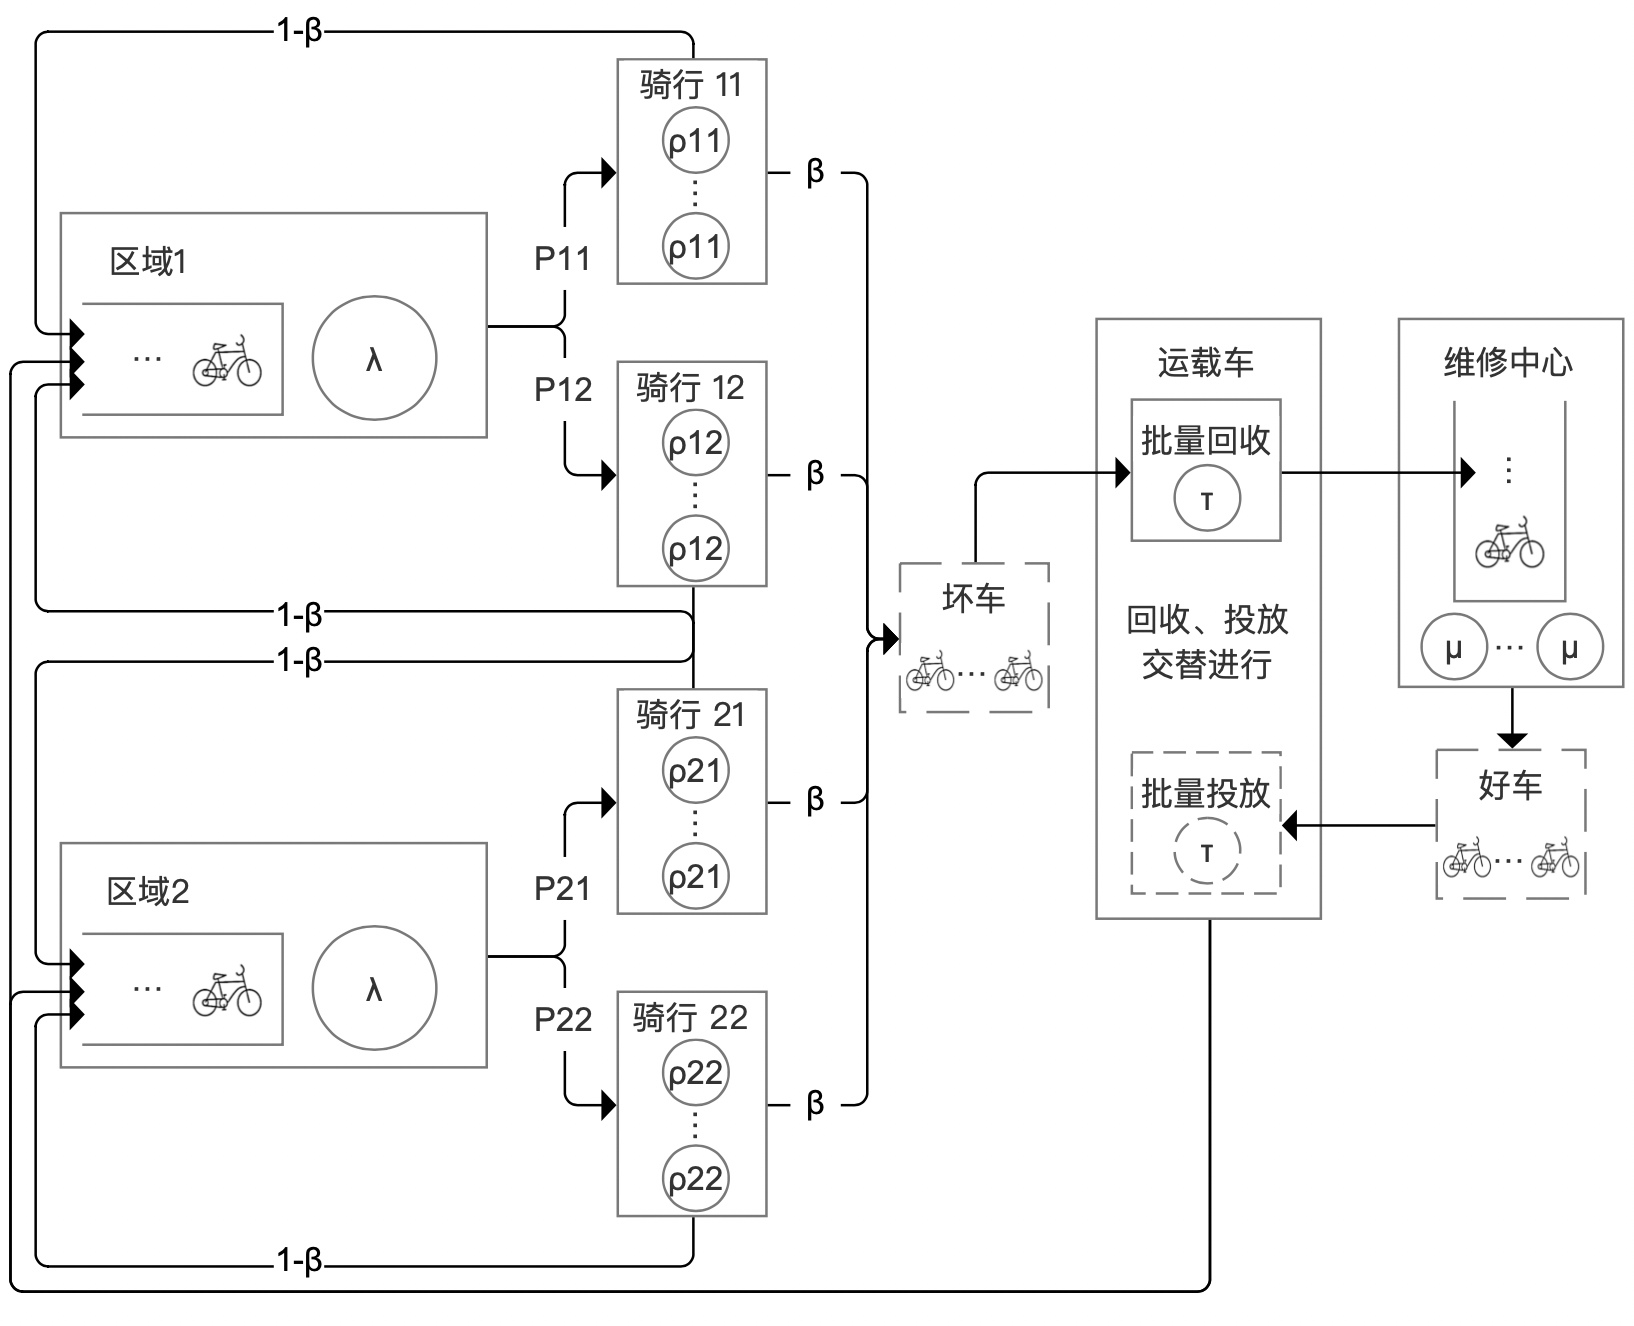
\includegraphics[scale=0.4]{./model/model.png}
    \caption{共享单车运维排队网络建模示意图}
    \label{cenmodel}
\end{figure}

\subsection{符号标记}
表\ref{rvtable}和表\ref{paratable}分别给出系统状态变量的各分量描述和系统的各项参数。
\begin{table}[H]
    \centering
    \caption{状态随机变量分量表}
    \begin{tabular}{ |c|c| } 
     \hline
     符号 & 含义 \\ 
     \hline
     $i, j$ & 队列的脚标, $i,j = 1, \dots, A$ \\ 
     \hline
     $t$ & 系统时间变量\\ 
     \hline
     $N_i$ & 在队列$i$处的好车数\\
     \hline
     $R_{ij}$ & 正在被从$i$骑到$j$的车数 \\ 
     \hline
     $BP$ & 当前等待被运送至维修中心的坏车数 \\
     \hline
     $RC$ & 当前维修队列处的坏车数 \\
     \hline
     $DP$ & 当前等待被重新投放的坏车数 \\
     \hline
     $GD$ & 标记当前正在进行的过程是回收或是投放 \\
     \hline
    \end{tabular}
    \label{rvtable}
\end{table}

\subsubsection{系统参数}
\begin{table}[H]
    \centering
    \caption{参数表}
    \begin{tabular}{ |c|c|c| } 
     \hline
     参数 & 描述 & 默认值 \\ 
     \hline
     $A$ & 区域数 & 2 \\ 
     \hline
     $M$ & 总车数 & 6 \\ 
     \hline
     $\beta$ & 损坏概率 & 0.3 \\
     \hline
     $P_{ij}$ & 从i到j的骑行概率 & 随机数 \\
     \hline
     $\lambda_i$ & 区域i顾客到达速率 & 随机数 \\
     \hline
     $\rho_{ij}$ & 从i骑行到j的速率 & i,j的曼哈顿距离加一的倒数 \\
     \hline
     $\tau$ & 运维速率 & 1.0 \\
     \hline
     $C$ & 运载车容量 & 3 \\
     \hline
     $\mu$ & 单服务台维修速率 & 1.0 \\
     \hline
     $N$ & 服务台数量 & 1.0 \\
     \hline
    \end{tabular}
    \label{paratable}
\end{table}

\subsection{运维模型}
将在各队列中的自行车数作为状态向量的元素,我们使用$$\boldsymbol{X}_t = (N_1, \dots, N_{i}, \dots, N_A, R_{11}, \dots, R_{ij}, \dots, R_{AA}, BP, RC, DP)_t$$ 来表示系统在任意时间$t$的状态。

共享单车可以在各个区域中被骑行,从一个区域到达另一个区域或到达自身。骑行的时间根据区域间的距离不同,服从一定的指数分布。因而任意两个区域间相当于存在一个$M/M/\infty$队列。一次骑行完毕后,单车到达某个区域,进入这个区域的等待队列。每个区域的顾客到达服从一定参数的泊松分布。于是相当于可以服务的单车到达一个区域时进入一个$M/M/1$队列进行等待。当这个等待队列中没有单车时,新到达的顾客马上流失。当单车骑行完毕时也有可能进入损坏状态,此时其进入一个回收池\textit{Broken Pool}(简记为$BP$)。运载车负责将系统中损坏的单车回收运送至维修中心,和将维修中心处维修完毕的好车重新投放到运营之中。这里以\textit{Distribute Pool}(简记为$DP$),表示待投放的单车数量。运维车的操作时间服从参数为$\tau$的指数分布。也即,每隔一个参数为$\tau$的指数分布时间,运维车会搬运运载能力以内的尽可能多的坏车转移至维修中心,之后再经过参数为$\tau$的指数分布时间,维修后的好车被重新通入运营,这两个过程交替反复进行。通常在日常运行中还有一项工作是,搬运各个区域中分布的好车,以使各个区域中的可使用的单车数量尽可能满足该区域的骑行需求。因为通常现实中单车的调度也不是持续不断的进行的,而是隔一段时间进行,或者夜间进行,在调度过程中可以看做是不受控制的运行。或者根据实际运行情况,某个区域当前或者预期需求持续得不到满足,而需要往这个区域调配车辆。投放策略本身是一个重要的、值得研究,并且已经有很多研究的工作\cite{Caggiani2018A} \cite{温惠英2014基于迭代回归法的公共自行车投放量预测研究}。在本文中不作为重点讨论对象。为简化问题,转而采用一种较固定的可行策略:根据各个区域的顾客到达率和单车总数设置各个区域的目标数量,之后的投放以此为目标数量。需要注意的是,为了模型的精简,这里的回收和重新投放过程,对现实中的操作进行了简化和抽象。只为了抓住批量化回收的特征和用参数去刻画回收和投放的能力强弱。由以上我们可以描述封闭排队网络模型所对应的连续时间马尔可夫过程。
% Liu Asymmetric demand patterns often lead to imbalanced bike distributions (for both stationed and stationless systems), necessitating relocation of bikes to meet the expected future demand. This is a major operational problem and crucial for reducing customer dissatisfaction due to unmet demand (Kaspi, Raviv, & Tzur, 2017). For instance, in 2016, CitiBike rebalanced about a million bikes. As an example of these studies, O’Mahony and Shmoys (2015) develop integer programming formulations to optimize rebalancing operations to prepare for rush hours. Some studies consider rebalancing incentives (i.e., static and dynamic pricing schemes), for example, when riders are offered discount to pick up/drop off bikes from/at nearby stations that are full/empty or expected to become full/empty in the near future (Fricker, Gast, 2016, Haider, Nikolaev, Kang, Kwon, 2018, Patel, Qiu, Negahban, 2019). Several studies focus on vehicle routing and station prioritization to determine how rebalancing should be performed so as to minimize cost or rate of lost demand (Bulhoes, Subramanian, Erdogan, Laporte, 2018, Legros, 2019, Schuijbroek, Hampshire, van Hoeve, 2017).
由于每个队列处的服务时间的马尔可夫性,系统状态整体是一个连续时间马尔可夫链(Continuous-Time Markov Chain, CTMC)。因为好车可以以一定概率在任意区域之间被骑行,损坏了的车,将在维修后重新投放至各区域。

由于时间发生时间的随机性,并且单车可以在好坏状态之间进行转换,显然系统中任意一个状态可以以一定概率经过一定时间后转移到任意另一个状态。因此,这是一个遍历(Ergotic)的马尔可夫链。由马尔可夫链的性质,系统存在长程稳定状态。由此,我们在给定系统参数设置下,可以通过系统状态概率转移方程,求解系统处于各个状态概率,从而得到系统性能指标。

\subsection{决策模型}
在单车的日常运营中需要确定采用多少运载能力和维修能力。在本模型中主要包括运载车的数量和运维中心需要多少维修工人。基于前述建模的系统性能参数仍难以进行显式的表达,也因而难以直接作为目标函数进行优化。但是通过仿真的方法,可以较方便地获得系统性能参数。通过对前述仿真模型的扩展,可以轻易仿真系统中有多辆运载车同时运行的情况。系统中可分配到运载车和维修人员的资源预算为给定的有限值。不同运载量运载工具的单位平均成本,单位维修人员的成本也作为默认值给定。
在本文中我们主要关注最小化系统中顾客损失。对应的变量如表所示。
\begin{table}[H]
    \centering
    \caption{决策问题相关变量表}
    \begin{tabular}{ |c|c| } 
     \hline
     符号 & 含义 \\ 
     \hline
     $n_R$ & 决策变量,维修中心服务台的数量,正整数\\ 
     \hline
     $n_C$ & 决策变量,运载车的数量,正整数\\ 
     \hline
     $Cost_R$ & 单位维修中心服务台成本\\ 
     \hline
     $Cost_C$ & 单位运载车成本\\
     \hline
    %  $G(n_R, n_C; Cost_{R}, Cost_C)$ & 成本函数,$G = n_R Cost_{R} + n_C Cost_C$\\
    %  \hline
     $T$ & 预算总数 \\ 
    %  \hline
    %  $\delta$ & 无差别阈值 \\ 
     \hline
    \end{tabular}
    \label{tab:rv}
\end{table}

需要求解的问题如下:

\begin{align*}
    & \mathop{\arg\min}\limits_{n_R, n_C} \mathbb{E}[\mbox{顾客损失比例}]\\
    & \begin{array}{r@{\quad}r@{}l@{\quad}l}
    s.t.& n_R Cost_{R} + n_C Cost_C &\leq T\\
     &n_R, n_C&\in\mathbb{N}^+\\
    \end{array} 
\end{align*}

\section{模型求解}
在本部分,首先给出一个基于马尔可夫链长程稳态概率的系统性能求解方法。对于一个遍历的连续时间马尔可夫链,当时间趋向于无穷大时,系统处于各个状态的时间比例收敛于其极限概率。我们通过构建系统的状态转移概率方程,求解得到系统处于各状态的长程比例,并由此给出性能指标计算公式\cite{SheldonM2011应用随机过程}。

上述马尔可夫链的状态数量可通过系统中的区域数量、车的总数和运载车的数量计算得到,为$ 2^C \times \binom{A+A^2+3+M}{M}$。这意味着状态数量随区域数量、车的总数和运载车的数量的增长呈指数增长。于是,该系统对应的多元线性方程组将变得非常庞大,而难以求得精确解。而仿真的方法计算系统的性能参数,可以无需知晓所有状态,从而较快地收敛。因此,我们提出离散事件仿真的方法,计算得到系统的性能参数。

本文所要求解的决策问题的解空间为有限、离散的情况。对每一组解,由于随机性,仿真的结果会存在波动。每一组参数设置下的期望系统性能参数难以通过比较仿真实验的均值直接得到。我们使一种排选算法(Ranking and Selection Algorithm),Kim和Nelson在2001年提出的Fully Sequential, Indifference-Zone Method,求解本文的决策问题。

\subsection{CTMC状态方程求解方法}
记$S$为系统所有可能的状态的集合, $s$为集合中元素。记$$s^{T} = (N_1, \dots, N_A, R_{11}, \dots, R_{AA}, BP, RC, DP, GD)^{T}$$为系统状态向量。对于一个排队过程,由系统状态转移的偏微分方程可以构建任意系统状态其转出率与转入率相等的方程。因为系统中的总的车数固定,所以其符合下式:
\begin{equation}
    \left\{
        \begin{array}{lcl}
            \sum \limits _{i \in [1,A]}(N_i+\sum \limits _{j \in [1,A]}R_{ij})+BP+RC+DP = M; \\
            N_i, R_{ij}, BP, RC, DP\mbox{为}[0,M]\mbox{间的正整数}.
        \end{array}
    \right .
\end{equation}
\begin{equation}
    GD = \left\{
        \begin{array}{lcl}
            0, &\mbox{坏车搬运} \\
            1, &\mbox{好车投放}.
        \end{array}
    \right .
\end{equation}

记$\pi_s$为状态$s$的极限稳态概率。我们记$I_{N_i}$,$I_{BP}$和$I_{DP}$如下:
\begin{equation}
I_{N_i}=\left\{
    \begin{array}{lcl}
        1, &N_i > 0;\\
        0, &\mbox{否则}.
    \end{array}    
\right.
\end{equation}
% \begin{equation}
% I_{Operation}=\left\{
%     \begin{array}{lcl}
%         1, &I=0\mbox{且}BP>0 \mbox{或} I=1\mbox{且}DP>0;\\
%         0, &\mbox{否则}.
%     \end{array}    
% \right.
% \end{equation}


由马尔可夫链的性质,系统稳态下任意状态的转出速率为该状态可以到达的任意下一状态的长程比例乘以相应转移速率之和。即:
\begin{equation}
Rate-out_{s} = (\sum \limits _{i \in [1,A]}\lambda_i I_{N_i}+\sum \limits _{i \in [1,A]} \sum \limits _{j \in [1,A]} \rho_{ij} R_{ij}+\lambda +\mu \min \{RC, N\} + \tau )\pi_s.
\end{equation}
我们记示性函数$F_{s^{'}}$如下,其表示一个状态是否是可能存在的,存在为1,不存在为0.
\begin{equation}
F_{s^{'}}=
    \left\{
        \begin{array}{lcl}
            1, &\sum \limits _{i \in [1,A]}(N_i+\sum \limits _{j \in [1,A]}R_{ij})+BP+RC+DP= M;\\ & N_i, R_{ij}, BP, RC, DP\mbox{为}[0,M]\mbox{间的正整数};\\
            0, &\mbox{否则}.
        \end{array}
    \right .  
\end{equation}
同样由马尔可夫链的性质,系统稳态下任意状态的转入速率为任意可以到达该状态的上一状态的长程比例乘以相应转移速率之和。而投放前各区域的好车数需要由投放策略倒推得到。本文中采取根据各区域顾客到达率按比例分配的策略。初始目标投放量根据每个区域的到达速率按比例进行设置。在每次投放时,按照每个区域的到达率从高到低排序,依次检查区域中当前的好车数是否达到原始设定的目标值,如果没有达到则尽可能补充到目标值。再投放下个区域。直到待投放的好车数为0或所有区域已检查过。根据这个策略可以得到所有可能的投放前系统状态集合$Q$。

则马尔可夫过程稳态情况下任意系统状态,可能由另一个状态经由(1)顾客骑走一辆好车;(2)骑行到达;(3)骑行损坏;(4)坏车运送至维修中心;(5)维修完毕进入投放队列;(6)投放至各区域,这六种过程的某一种而进入。从而确定系统某状态的转入速率为:
\begin{equation}
    \begin{aligned}
        Rate-in_{s} &= 
        \sum \limits _{i \in [1,A]} \sum \limits _{j \in [1,A]} \lambda_i P_{ij} \pi_{(\dots, N_i+1, \dots ,R_{ij}-1,\dots)} F_{(\dots, N_i+1, \dots ,R_{ij}-1,\dots)}\\
        &+\sum \limits _{i \in [1,A]} \sum \limits _{j \in [1,A]} \rho_{ji} R_{ji} (1-\beta) \pi_{(\dots, N_i-1, \dots ,R_{ij}+1,\dots)} F_{(\dots, N_i-1, \dots ,R_{ij}+1,\dots)}\\
        &+\sum \limits _{i \in [1,A]} \sum \limits _{j \in [1,A]} \rho_{ij} R_{ij} \beta \pi_{(\dots ,R_{ij}+1, \dots, \dots, BP-1, \dots)} F_{(\dots ,R_{ij}+1, \dots, \dots, BP-1, \dots)}\\
        &+\tau \sum \limits _{B \in [1,\min\{C, RC\}] } \pi_{(\dots, BP+B, RC-B, \dots, GD=1)} \\
        &+\mu \min \{RC, N\} \pi_{(\dots, RC+1, DP-1)} F_{(\dots, RC+1, DP-1)}\\
        &+\tau \sum \limits _{q \in Q}\pi_{q} F_{q}\\
    \end{aligned}
\end{equation}
又有:
\begin{equation}
    \sum \limits _{s \in S} \pi_{s} = 1
\end{equation}
通过联立前述(1)-(7)式可以求解以上系统状态转移概率方程组,得到系统处于每个状态的长程比例。

\subsubsection{系统运行指标计算}
根据系统的每个状态的长程稳态概率,可以计算得到如下系统性能指标。

\textbf{1、期望顾客损失率}
当系统中某个区域处没有好车时,新到达的顾客将会损失掉。因此通过没有好车的区域的顾客到达速率除以总的顾客到达速率可以得到期望任意状态的顾客损失比率例。再通过对所有状态加权平均即可得到期望顾客损失率。
\begin{equation}
E[\mbox{顾客损失率}] = \frac{1}{M} \sum \limits _{s \in S} \pi_{s} \sum \limits _{N_i \in s} I(N_i) \lambda_i / \sum \limits _{i \in [1,A]} \lambda_i 
\end{equation}

\textbf{2、期望好车比例}
系统中好车和坏车的比例可以由任意状态中的好车数量占车总数的比例求期望平均得到。
\begin{equation}
    E[\mbox{好车比例}] = \frac{1}{M} \sum \limits _{s \in S} \pi_{s} \sum \limits _{N_i \in s} N_i 
\end{equation}

\textbf{3、期望维修服务台闲置率}
维修中心处可能会有多台服务台。当维修中心处待维修的单车数少于维修台数量时,即出现了服务台的闲置。因此通过维修中心处的车数除以服务台数得到某一状态的限制比例,再通过对所有状态平均,即可得到期望维修服务台闲置率。
\begin{equation}
E[\mbox{维修服务台空置率}] = \sum \limits _{s \in S} \pi_{s} (1 - RC^s / N)
\end{equation}


\subsection{仿真方法}
通过设置系统的状态转移规则,我们可以模拟前述提出的单车系统模型。通过向模型输入符合分布假设的随机数,可以模拟所建立的模型对应的系统的运行。当系统存在大量状态时,无论是方程求解还是在仿真中确保所有状态都被访问到,都需要大量时间。而实际系统无需访问大量状态,系统的性能指标也已进入稳定状态。基于仿真的方法可以较快地得到我们关心的系统性能指标。后文数值计算部分通过设置同样的参数,对比方程求解结果和仿真结果,验证了CTMC模型ODE方程求解方法与仿真方法的一致性。

在仿真中,通过记录系统状态的变化和状态持续时间,可以计算得到仿真进行到某一时刻为止,系统中好车比例的均值和维修中心闲置比例的均值;通过记录的到达顾客总数和未被服务而而丢失的顾客总数相除,可以计算得到顾客损失比例。从而观察系统性能指标均值随时间的变化。观察这些指标随仿真运行时间的变化,可以判断系统是否进入稳态。取系统进入稳态后的一段时间,计算这段时间某性能指标的平均作为该指标的期望值\cite{welch1983statistical}。


\subsection{排选算法}
Kim与Nelson在他们的工作中提出了Fully Sequential, Indifference Zone Method\cite{Kim2001A},该算法可以以设定的置信度$1-\alpha$从候选系统中挑选出均值最优的系统。参数$\delta$表示无差别区间长度,当两个待选系统在性能表现差距在$\delta$以内时,认为两个系统的性能表现相同。表现在结果上是当某些系统的均值与最优系统对应的均值之间的距离小于该值时,多次执行算法,这些系统也将被当做最优系统而以一定频率被选出。该方法的优点在于,首先,可以设置无差别区间,从而可以认为决定什么样程度的性能差别是没有影响的;其次,其筛选过程中,可以逐步剔除明显差的方案,从而节省比较所需要的总样本数;而且,该方法虽然基于样本分布为正态的假设,但是对样本分布非正态有着较好的抵抗力。可以应对在实际使用过程中,样本分布的未知性。
算法的参数输入如下表。
\begin{table}[H]
    \centering
    \caption{算法输入参数表}
    \begin{tabular}{ |c|c|c| } 
     \hline
     符号 & 含义 & 默认值\\ 
     \hline
     $ k $ & 待比较系统数量 & 随问题变化\\ 
     \hline
     $ 1-\alpha $ & 置信度 & 0.05 \\ 
     \hline
     $ \delta $ & 无差别区域宽度 & 0.01\\ 
     \hline
     $ n_0 $ & 初始样本量大小,$ n_0 \geq 2 $ & 20 \\ 
     \hline
     $ c $ & 算法参数 & c = 1 \\ 
     \hline
     $ i $ & 第i个系统 & $ i = 1, 2, \dots, k. $ \\ 
     \hline
     $ j $ & 第j次观测 & $ j = 1, 2, \dots, n_0. $ \\ 
     \hline
    \end{tabular}
    \label{tablerv}
\end{table}
记$X_{ij}$为系统$i$的第$j$个观测值。
算法流程如算法\ref{algo}所示。
\begin{algorithm}  
    \caption{Fully Sequential, Indifference-Zone Procedure}  
    \begin{algorithmic}[1] %每行显示行号  
        \Require $k, alpha, \delta, n_0, c, X$ 
        \Ensure 最优系统编号\\
        \textbf{初始化:}\\
            $I = \{ 1,2, \dots, k\}$ \\
            $\eta = \frac{1}{2} [(\frac{2 \alpha}{k - 1})^{-2/(n_0-1)} - 1]$ \\
            $h^2 = 2 (n_0 - 1) c \eta $\\  
            $S _{il} ^{2} = \frac{1}{n_0 - 1} \sum \limits _{j=1} ^{n_0} 
            (X_{ij} - X_{lj} - [\overline{X} _i (n_0) - \overline{X} _l (n_0)]) ^2, 
            \  \forall \ i \in I \  and \  i \neq l $ \\
            $N_{il} = \lfloor \frac{h^2 S_{il}^2}{\delta ^2} \rfloor, 
            \  \forall \ i \in I \  and \  i \neq l $ \\
            $N_i = \max \limits _{l \neq i} N_{il}, \  \forall \ i \in I $ \\
            $\overline{X} _i (r) = \frac{1}{r} \sum _{j=1} ^{r} X_{ij}$\\
        \State
        \textbf{初始判断:}
            \If{$ n_0 > \max _i N_i $}  
                \State \Return{$\mathop{\arg\max} _i \overline{X} _i (n_0)$} 
            \Else  
                \State $ r = n_0 $
                \State 进入\textbf{筛选过程}
            \EndIf  \\
        \State
        \textbf{筛选过程:}
            \While{$|I| > 1$}
                \State $\forall$系统$i \in I$中添加一个观测值$X_{i, r+1}$
                \State $r = r+1$
                \If{$r == \max _i N_i + 1$}  
                    \State \Return{$\mathop{\arg\max} _i \overline{X} _i (r)$}  
                \Else  
                    \State $ I^{old} = I $
                    \State Update $ \overline{X} _i (r), \  \forall i \in I$
                    \State $W _{il} (r) = \max \{ 0, \frac{\delta}{2cr} (\frac{h^2 S ^2 _{il}}{\delta ^2} - r)\}, \  \forall \ i \in I \  and \  i \neq l $
                    \State $ I = \{i : i \in I^{old} \quad and \quad \overline{X} _i (r) \geq \overline{X} _l (r) - W_{il} (r), \forall l \in I^{old}, l \neq i\} $
                \EndIf  
            \EndWhile  
            \State \Return{$I$}
    \end{algorithmic}  
    \label{algo}
\end{algorithm}  


\section{数值计算}
\subsection{运维模型求解}
首先通过离散系统仿真的方法,给系统设置如表\ref{rvtable}和\ref{paratable}所示的默认系统参数。初始系统中所有车均为可骑状态,并且平均分布于各个区域中。
\begin{figure}[H]
    \centering
    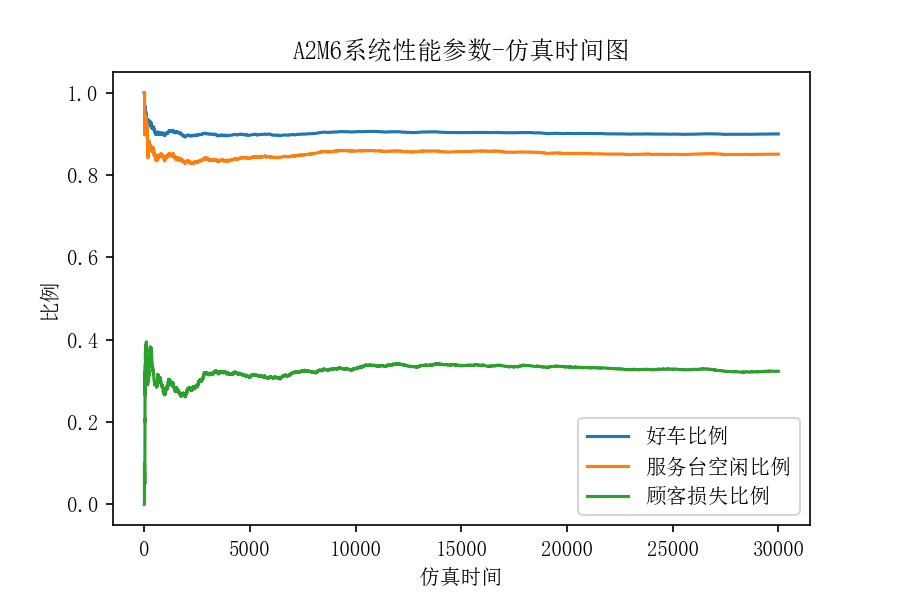
\includegraphics[scale=0.5]{sim/sim_timeA2M6.png}
    \caption{A2M6系统性能参数-时间30000图}
    \label{fig:cenmodel}
\end{figure}
通过设置相同的参数比较,方程求解结果与仿真结果。如下图所示:
\begin{figure}[H]
    \centering
    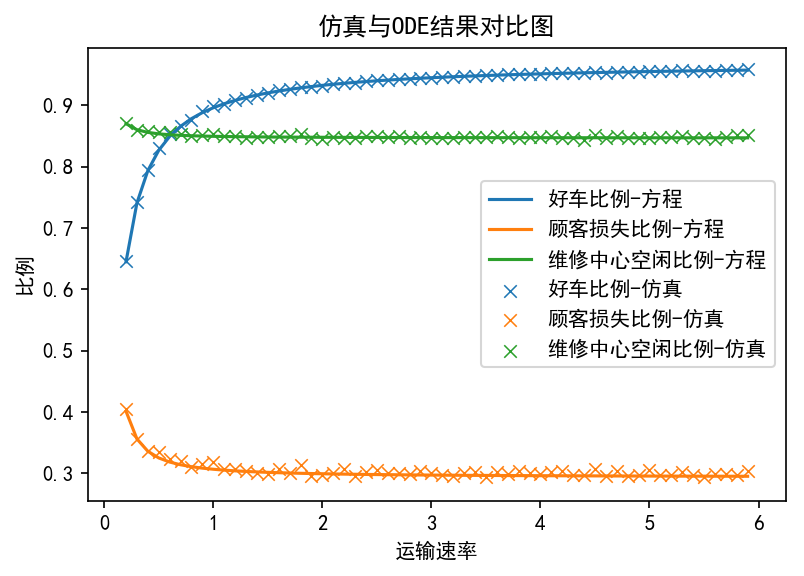
\includegraphics[scale=0.5]{A2M6仿真-odeSingle.png}
    \caption{A2M6方程与仿真结果对比图-变动运载服务台速率}
    \label{fig:cenmodel}
\end{figure}
\begin{figure}[H]
    \centering
    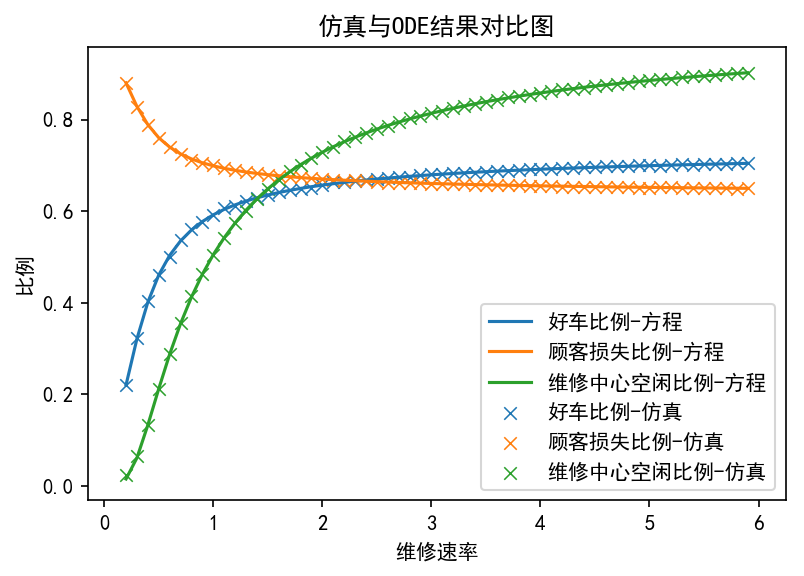
\includegraphics[scale=0.5]{A2M6仿真-odeSingleVaryMu.png}
    \caption{A2M6方程与仿真结果对比图-变动维修服务台速率}
    \label{fig:cenmodel}
\end{figure}
由上两幅系统性能参数随系统单服务台运维能力变化图可知,单独提升运维系统中的某个运维服务台的性能,可以提升系统的表现,但提升效果存在边际递减现象。

通过比较方程求解和仿真的结果可以看到,仿真的方法可以良好地逼近系统性能参数的理论值。而系统的状态数随着运载车数量每增加一辆就会翻倍,求解的时间也会大大增加。便利起见,以仿真的结果,研究系统中维修和运载服务台数量变化,引起的系统状态变化。
%改成黑白
\begin{figure}[H]
    \centering
    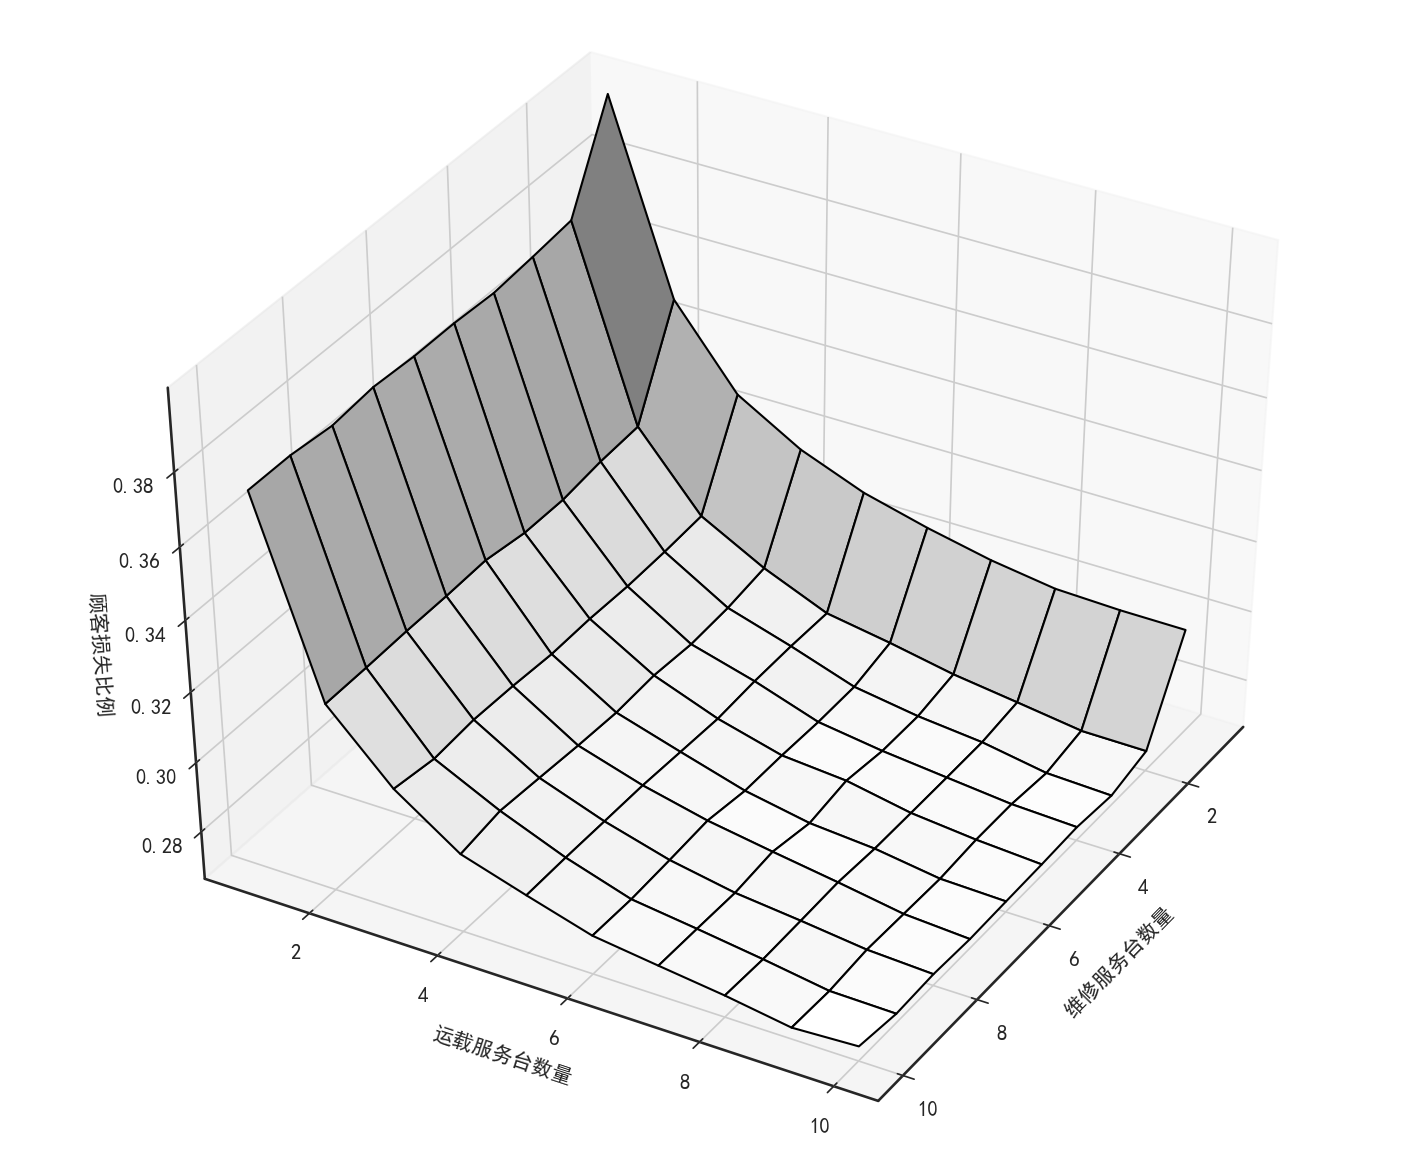
\includegraphics[scale=0.5]{A2M6VN3D.png}
    \caption{A2M6运载服务台与维修服务台数量对系统顾客损失比例影响}
    \label{fig:cenmodel}
\end{figure}
从图中可以看到,单独增加维修或运载服务台的数量都可以使系统性能表现改善,但改善的效果逐渐减弱。当二者大到一定程度之后系统的性能表现几乎不再改善。由此可知,对一个共享单车运营系统而言,单纯通过增加维修或投放的能力对改善系统的性能表现是存在上限的。并且,过多的投入边际收益很低。


\subsection{决策模型数值结果}
本文所提出的两阶段算法,在第一阶段可以以一定概率保证选出最优方案,同时输出样本均值与最优方案相差在设定范围的方案集合。第二阶段通过计算方案集合中所有方案的成本,选择出成本最小的方案。
\subsubsection{排选算法验证}
我们首先在A=2,M=6的条件下,求解只有一辆运载车时的退化决策问题以比较理论计算与排选算法的结果。
\begin{figure}[H]
    \centering
    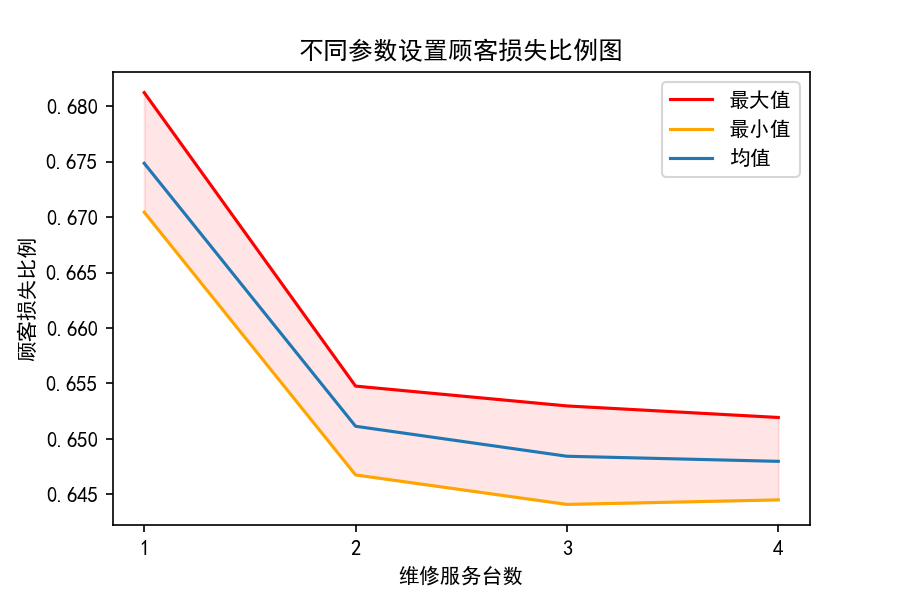
\includegraphics[scale=0.5]{A2M6RS验证图.png}
    \caption{A2M6方程与仿真结果对比图-变动维修服务台数量}
    \label{a2m6rsyz}
\end{figure}
如图中所示,当系统中维修服务台数量为3和4时,系统的性能指标非常接近。方程理论计算结果显示服务台数量为4时,系统性能表现最好,但二者之间的差距非常小。
\begin{figure}[H]
    \centering
    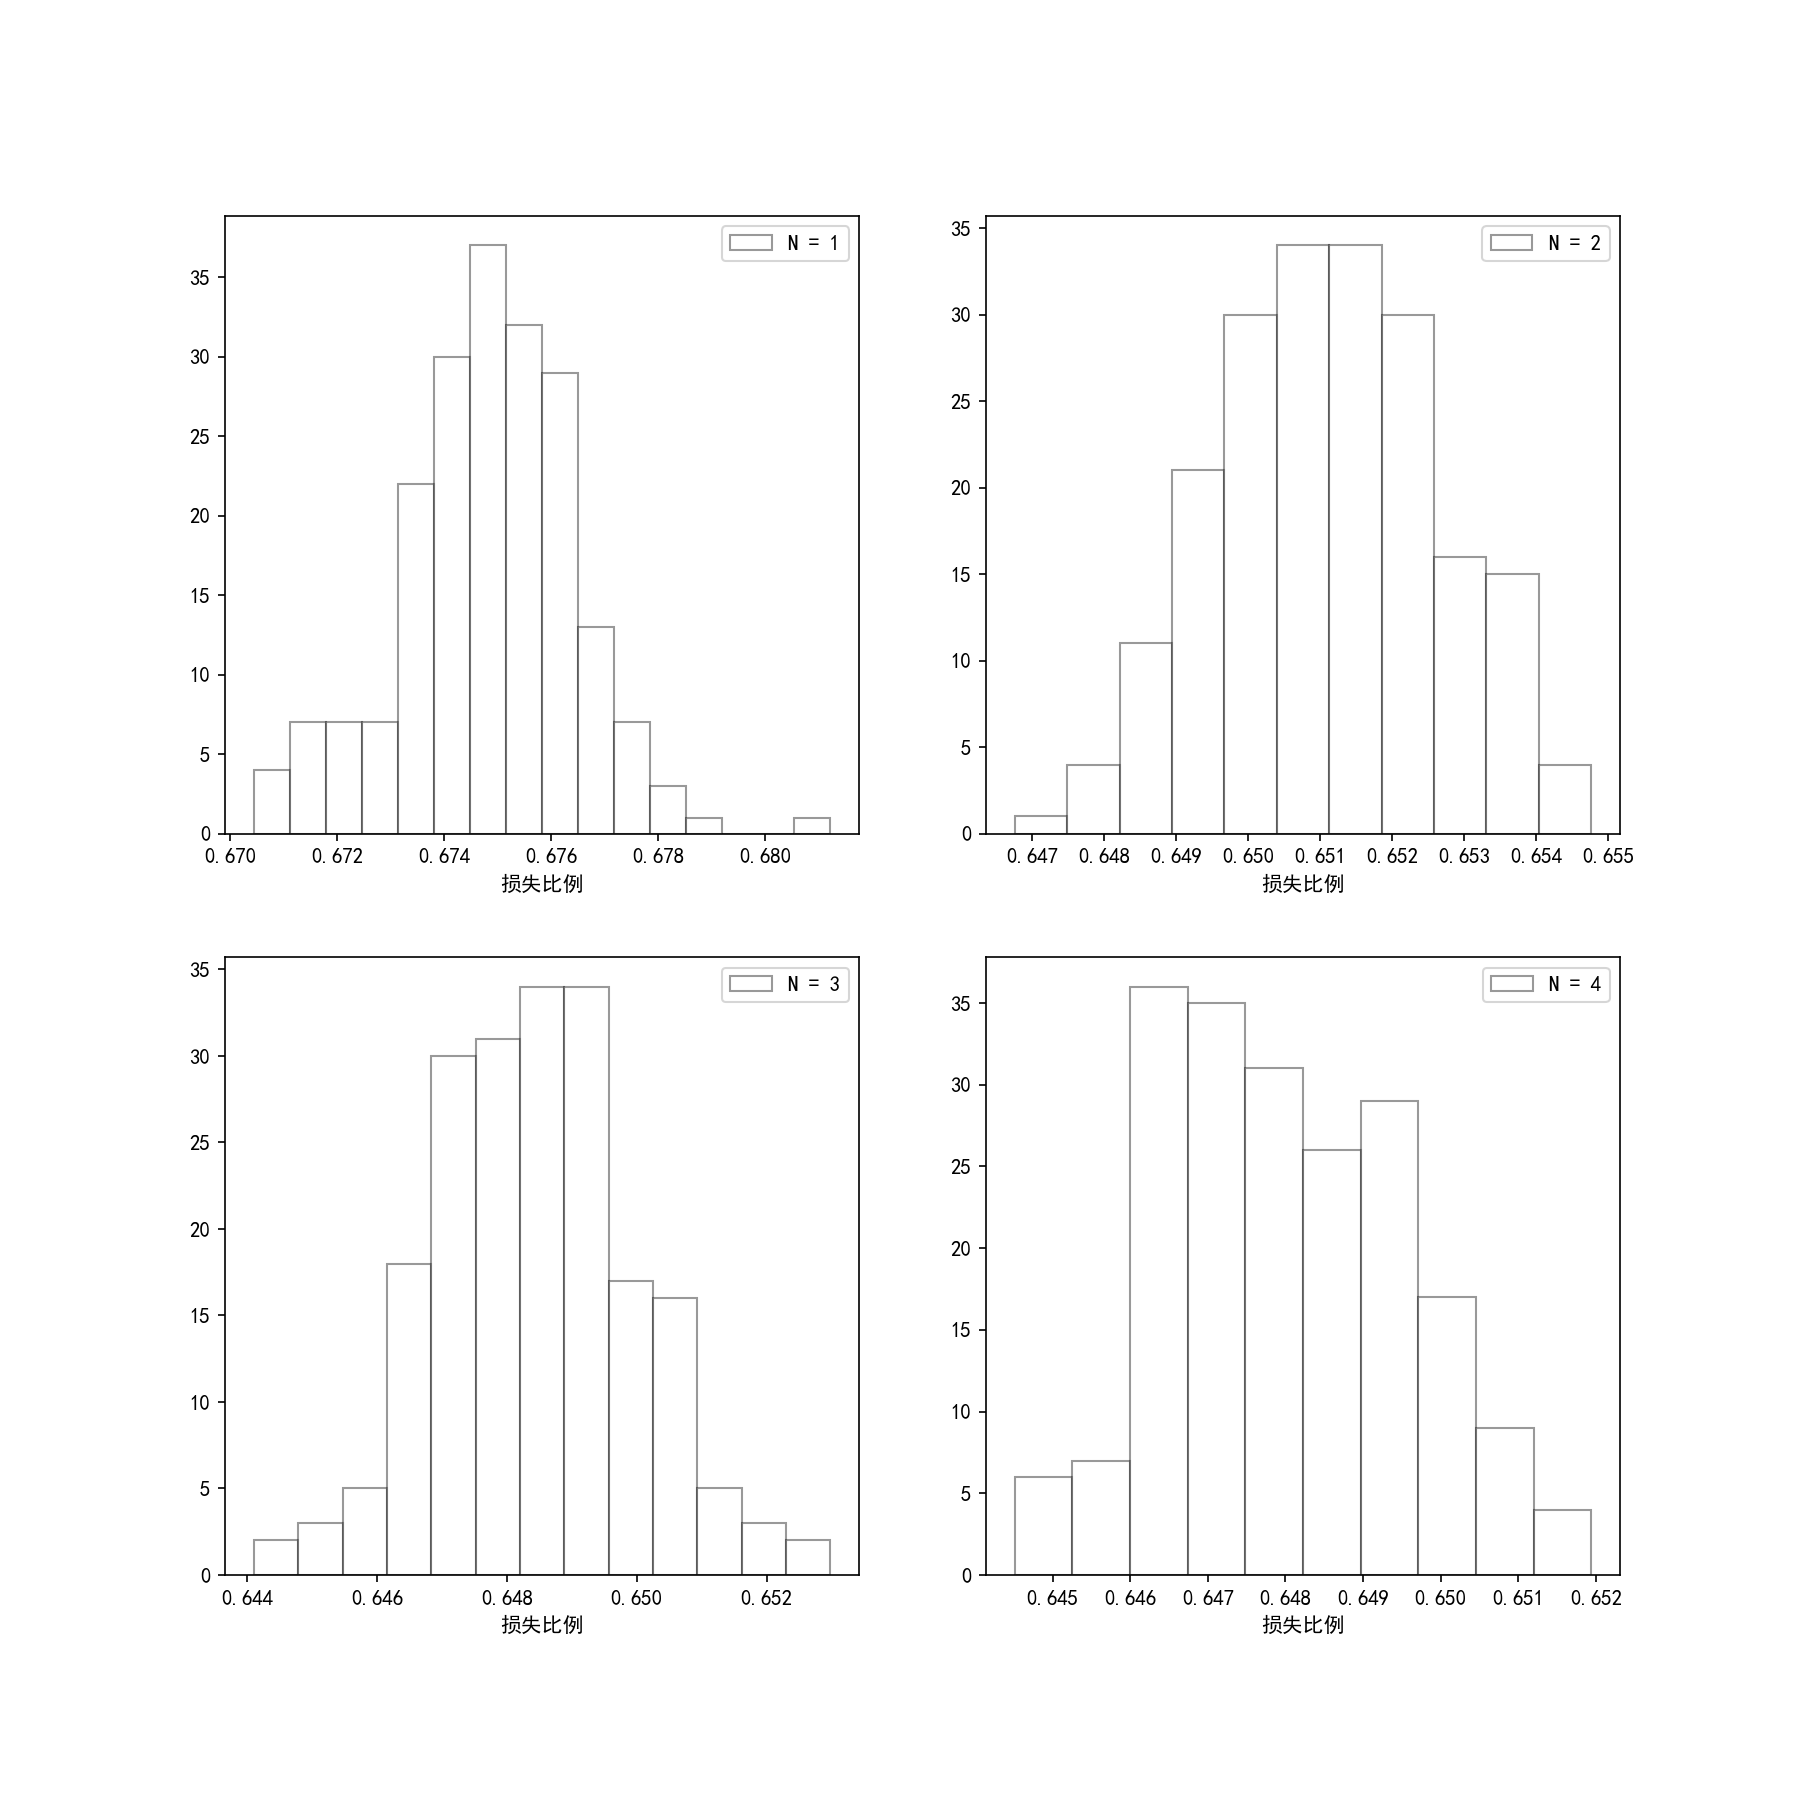
\includegraphics[scale=0.5]{A2M6NormalityTest.png}
    \caption{A2M6仿真结果频数统计图}
    \label{normaltest}
\end{figure}
图\ref{normaltest}为不同服务台数量情况下仿真结果的分布。结果均能通过正态性的KS检验。可以认为排选算法适用于该问题。为了使正态性得到更好地保证,所有排选算法均以3次试验观测值的样本均值作为一个数据点。按照前述参数表中的算法参数设置,运行1000次排选算法,结果N=4被选中974次,N=3选中26次。验证了算法的正确性。

\subsubsection{数值算例}
分别在A=2,M=6和A=10,M=100的情况下,设置不同的随机种子,初始化不同转移概率和到达率,作为待比较方案。在如表\ref{tablerv}所给出的参数设置下,运行500次排选算法,以出现次数最多的方案为最佳结果。与此同时,我们计算每个方案100次试验的均值,记为简单均值,以此为排名参照标准,与排选结果进行比较。结果如表\ref{a2m6rs}所示。
\begin{table}[H]
    \centering
    \caption{A=2,M=6时排选算法与样本平均结果表}
    \begin{tabular}{ |c|c|c|c|c|c|c|c| } 
     \hline
     随机种子 &  \tabincell{c}{排选最优结果\\ ($n_R, n_c$)} & 被选次数 & 平均使用样本数 & \tabincell{c}{样本均值最优方案\\ ($n_R, n_c$)} & \tabincell{c}{最优方案\\ 样本均值} & \tabincell{c}{简单均值\\ 样本数} \\ 
     \hline
    %  1 & 3, 7 & 0.119395 & 1, 3 & 0.122552 & 60.00 \\ 
    %  \hline
     %1 & (2,8):347;(3,7):153 & (2,8):0.421530;(3,7):0.421830 & 1080 & (2,8) & 0.421530 & 4500 \\ 
     %\hline
     %2 & (2,7):157;(2,8):150;(3,7):100;(3,6):67;(4,6):24;(5,5):2 & (2,8):0.421530;(3,7):0.421830 & 1080 & (2,8) & 0.421530 & 4500 \\ 
     1 & (2,8) & 148 & 904 & (2,8) & 0.254980 & 4500 \\
     \hline
     2 & (2,8) & 343 & 900 & (2,8) & 0.421530 & 4500 \\ 
     \hline
     2 & (4,6) & 184 & 927 & (4,6) & 0.400928 & 4500 \\
     \hline
    \end{tabular}
    \label{a2m6rs}
\end{table}
\begin{table}[H]
    \centering
    \caption{A=10,M=100时排选算法与样本平均结果表}
    \begin{tabular}{ |c|c|c|c|c|c|c|c| } 
     \hline
     随机种子 &  \tabincell{c}{排选最优结果\\ ($n_R, n_c$)} & 被选次数 & 平均使用样本数 & \tabincell{c}{样本均值最优方案\\ ($n_R, n_c$)} & \tabincell{c}{最优方案\\ 样本均值} & \tabincell{c}{简单均值\\ 样本数} \\ 
     \hline
     1 & (7,3) & 500 & 900 & (7,3) & 0.843801 & 4500 \\
     \hline
     2 & (7,3) & 500 & 900 & (7,3) & 0.853247 & 4500 \\ 
     \hline
     2 & (7,3) & 422 & 900 & (7,3) & 0.854234 & 4500 \\
     \hline
    \end{tabular}
    \label{a10m100rs}
\end{table}
由数值实验结果可以看到,排选算法可以以较少的样本观测量要求,选出性能指标满足给定要求的方案。适用于实际中难以进行取样的复杂系统,进行若干方案中的可行方案的挑选。

\section{结论}
本文通过将共享单车的服务过程和坏车运维过程建模成封闭排队网络,将共享单车的运维建模成封闭的排队网络,构建了对应的连续时间马尔可夫过程。通过状态转移方程求得系统稳态概率和系统性能指标。并通过仿真方法模拟得到系统的性能指标。观察到共享单车运维系统中,单独提高系统的运载速率或增加数量,亦或是提升维修环节的速度或维修人员的数量,对系统的改善作用都存在边际递减现象。因此,在可分配资源总数有限的条件下,需要在维修和运载环节之间进行合理分配。由于系统的复杂性,理论求解难以进行,通过仿真的方法可以较好地获得系统性能指标。进一步结合排选算法,可以在给定置信度下,以较小的运算成本,确定可接受的最优方案。

\newpage
\bibliographystyle{plain}
\bibliography{references.bib}

% \newpage

% \textbf{English Abstract}



\end{document}
% \section{运维过程建模}
% 共享单车的有桩无桩模式相较有桩模式而言,单车的分布情况是比较散乱的。而在实际中,单车的运维往往是基于划分的区域进行的。为了研究方便,本工作将共享单车的运行区域抽象成一个个相邻的区域。加上单车的运维部分,整体构成共享单车的运行系统。如图\ref{fig:cenmodel}所示。通常情况下,共享单车采用集中式维修的模式。在该模式下,操作员使用运输工具将一定区域内无法使用的自行车收集起来进行集中维修。一些工人在维修中心维修后仍无法使用的自行车将被替换成新车。然后,维修好的自行车将被重新分配到各个区域。这样的过程一致持续进行。通常在日常运行中还有一项工作是,搬运各个区域中分布的好车,以使各个区域中的可使用的单车数量尽可能满足该区域的骑行需求。因为通常现实中单车的调度也不是持续不断的进行的,而是隔一段时间进行,或者夜间进行,在调度过程中可以看做是不受控制的运行。或者根据实际运行情况,某个区域当前或者预期需求持续得不到满足,而需要往这个区域调配车辆。在本文中,不是重点的讨论的对象。因此,只在单车重新投放时考虑根据各个区域的顾客到达速率进行按比例分配。本文构建了一个封闭排队网络研究该服务系统。

% \begin{figure}[H]
%     \centering
%     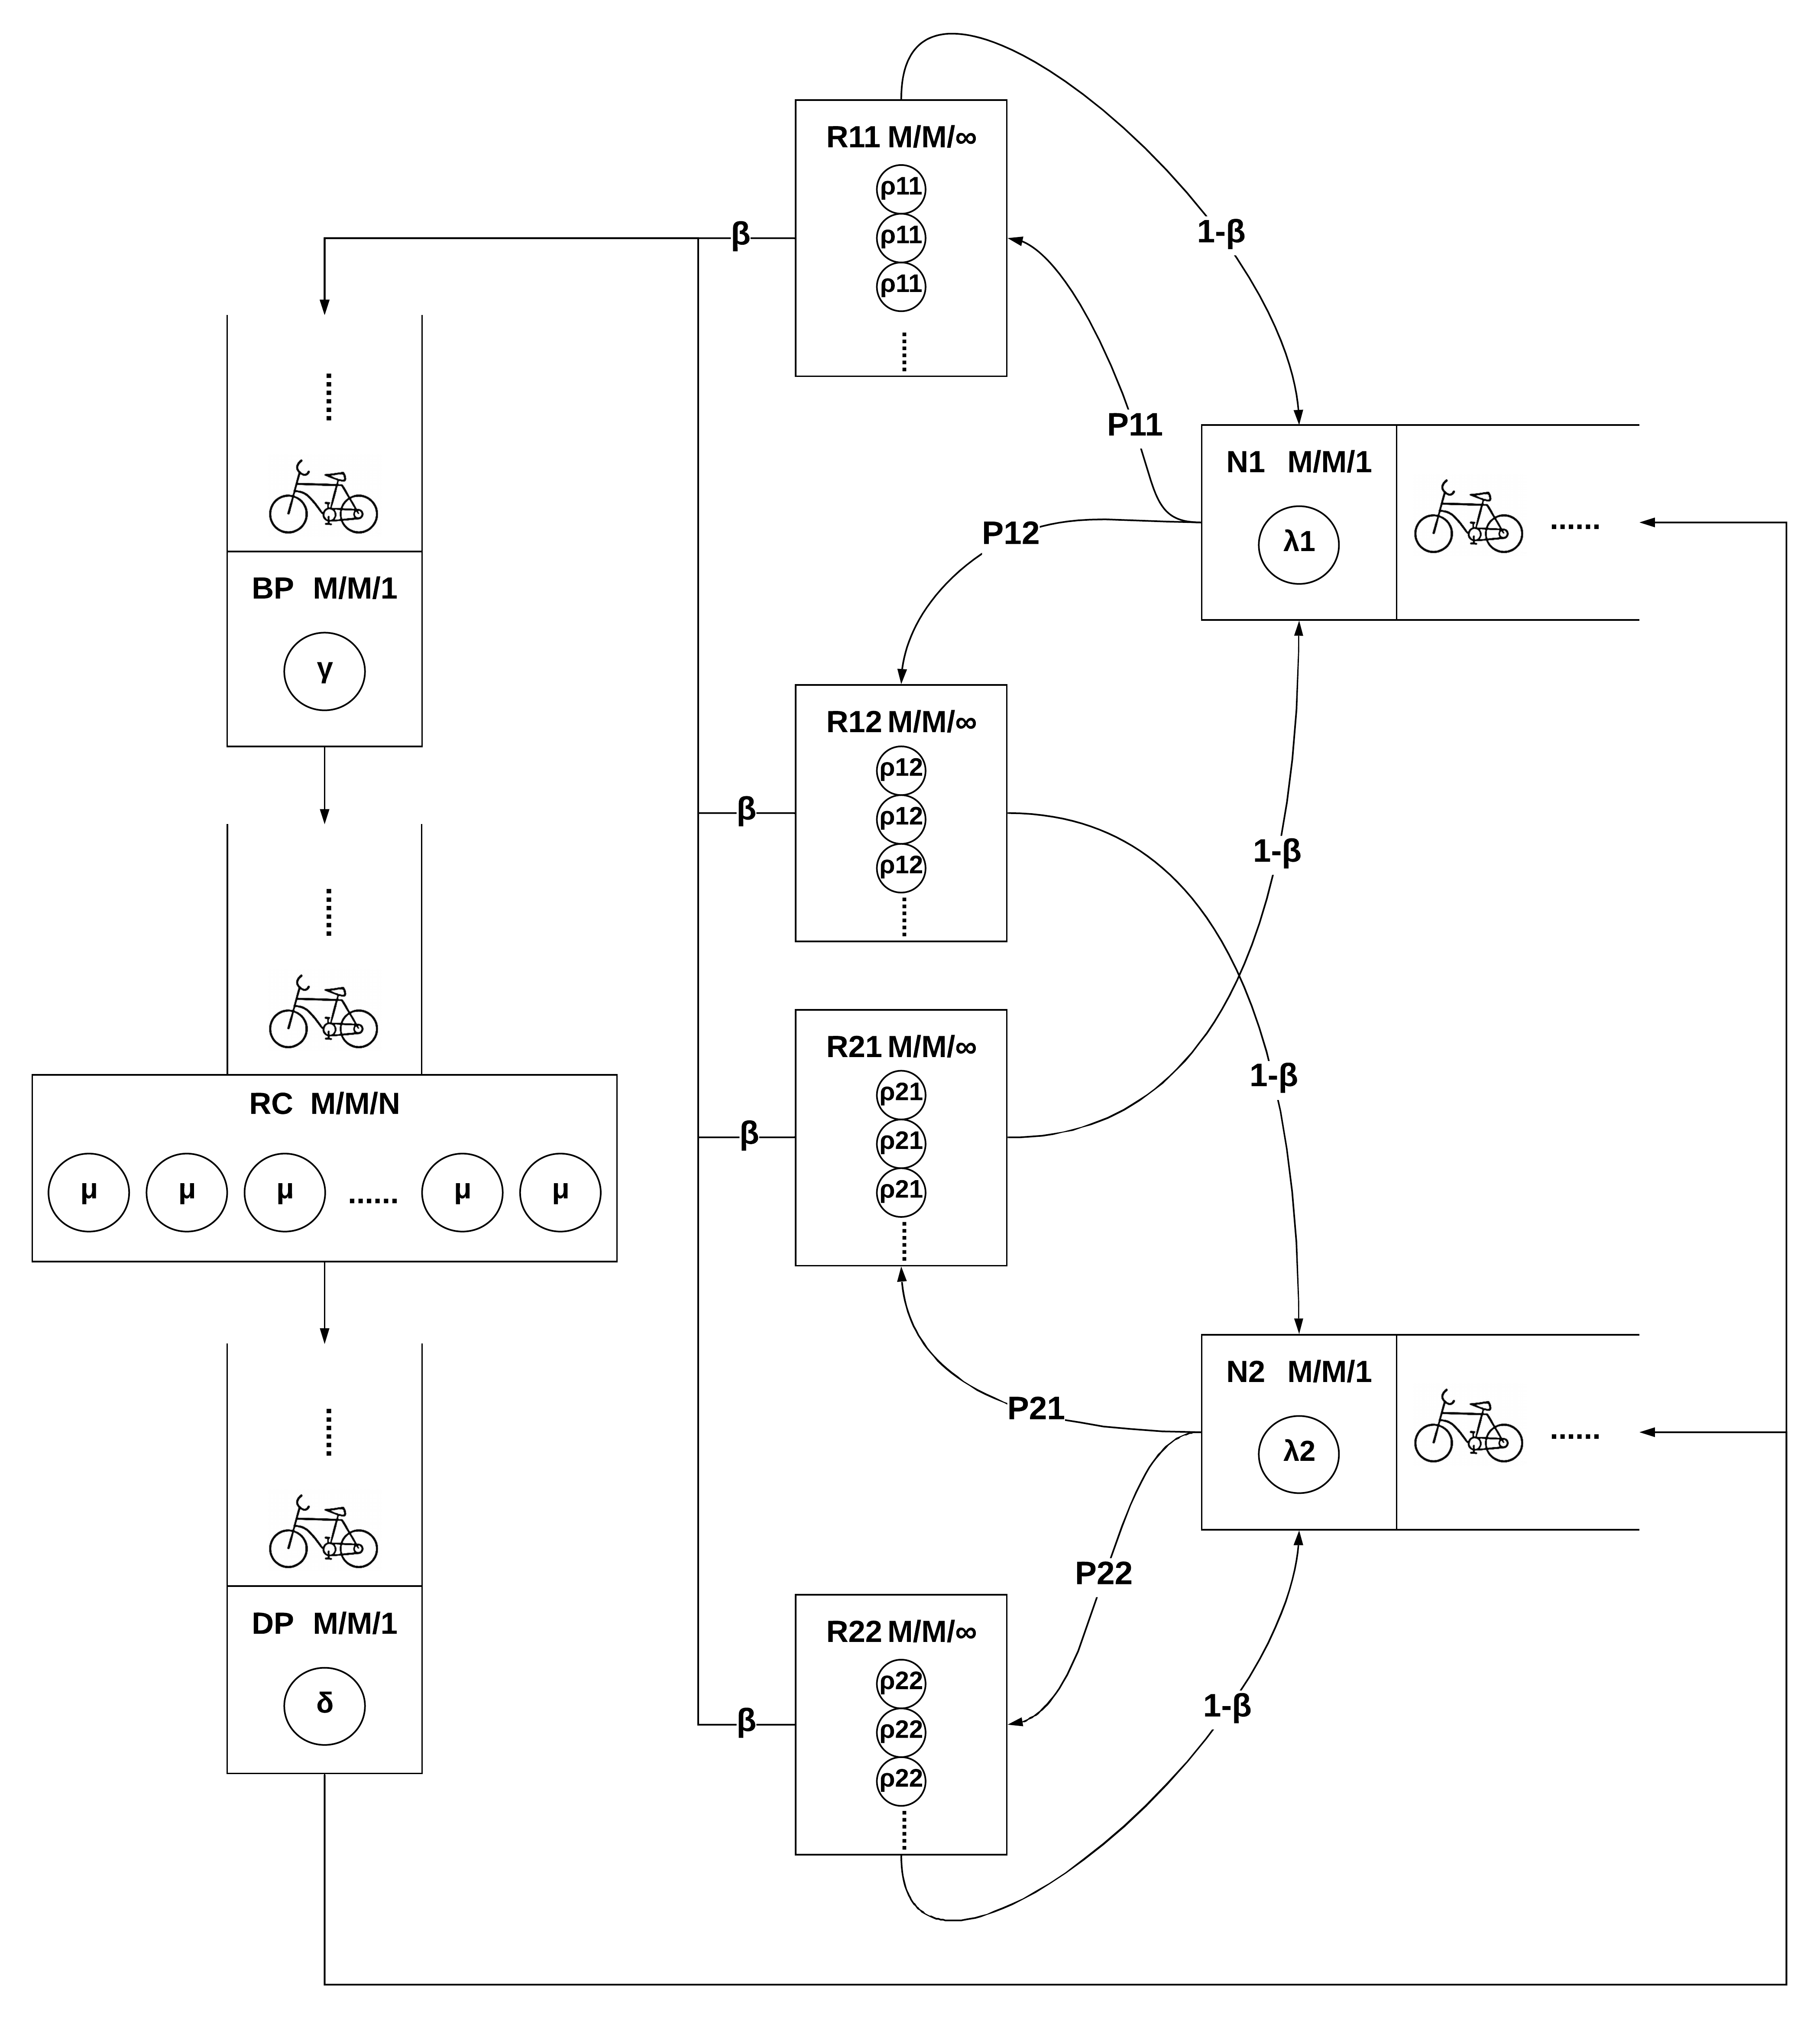
\includegraphics[scale=0.3]{CentralModel2.png}
%     \caption{共享单车运维排队网络建模示意图}
%     \label{fig:cenmodel}
% \end{figure}


% \subsection{符号标记}

% \subsubsection{随机变量}
% \begin{table}[H]
%     \centering
%     \caption{状态随机变量分量表}
%     \begin{tabular}{ |c|c| } 
%      \hline
%      符号 & 含义 \\ 
%      \hline
%      $i, j$ & 队列的脚标, $i,j = 1, \dots, A$ \\ 
%      \hline
%      $t$ & 系统时间变量\\ 
%      \hline
%      $N_i$ & 在队列$i$处的好车数\\
%      \hline
%      $R_{ij}$ & 正在被从$i$骑到$j$的车数 \\ 
%      \hline
%      $BP$ & 当前等待被运送至维修中心的坏车数 \\
%      \hline
%      $RC$ & 当前维修队列处的坏车数 \\
%      \hline
%      $DP$ & 当前等待被重新投放的坏车数 \\
%      \hline
%     \end{tabular}
%     \label{rv}
% \end{table}

% \subsubsection{系统参数}
% \begin{table}[H]
%     \centering
%     \caption{参数表}
%     \begin{tabular}{ |c|c|c| } 
%      \hline
%      参数 & 描述 & 默认值 \\ 
%      \hline
%      $A$ & 区域数 & 2 \\ 
%      \hline
%      $M$ & 总车数 & 6 \\ 
%      \hline
%      $\beta$ & 损坏概率 & 0.3 \\
%      \hline
%      $P_{ij}$ & 从i到j的骑行概率 & 随机数 \\
%      \hline
%      $\lambda_i$ & 区域i顾客到达速率 & 随机数 \\
%      \hline
%      $\rho_{ij}$ & 从i骑行到j的速率 & i,j的曼哈顿距离加一的倒数 \\
%      \hline
%      $\gamma$ & 回收速率 & 1.0 \\
%      \hline
%      $\overline{B}$ & 回收批量 & 1 \\
%      \hline
%      $\mu$ & 单服务台维修速率 & 1.0 \\
%      \hline
%      $N$ & 服务台数量 & 1 \\
%      \hline
%      $\delta$ & 投放速率 & 1.0 \\
%      \hline
%      $\overline{D}$ & 投放批量 & 2 \\
%      \hline
%     \end{tabular}
%     \label{para}
% \end{table}

% \subsection{运维模型}
% 单车运维系统可以看成由好车服务和坏车运维两个部分组成。每个部分由若干排队队列组成,整体构成封闭排队网络。将在各队列中的自行车数作为状态向量的元素,我们使用$$\boldsymbol{X}_t = (N_1, \dots, N_{i}, \dots, N_A, R_{11}, \dots, R_{ij}, \dots, R_{AA}, BP, RC, DP)_t$$ 来表示系统在任意时间$t$的状态。
% 共享单车可以在各个区域中被骑行,从一个区域到达另一个区域或到达自身。骑行的时间根据区域间的距离不同,服从一定的指数分布。因而任意两个区域间相当于存在一个$M/M/\infty$队列。一次骑行完毕后,单车到达某个区域,进入这个区域的等待队列。每个区域的顾客到达服从一定参数的泊松分布。于是相当于可以服务的单车到达一个区域时进入一个$M/M/1$队列进行等待。当这个等待队列中没有单车时,新到达的顾客马上流失。当单车骑行完毕时也有可能进入损坏状态,此时其进入一个回收池\textit{Broken Pool}(简记为$BP$)。当回收池中的坏车数量达到一定阈值$\overline{B}$,或者系统中已经没有好车,而回收池中有车时,这批坏车经过参数为$\gamma$指数时间后到达维修中心\textit{Repairing Center}(简记为$RC$)。维修中心处的维修过程相当于$M/M/N$的排队过程。有$N$个服务台负责对单车进行维修,每个服务台的维修时间服从相同的指数分布。当单车维修完毕后,随即进入一个投放池\textit{Distribute Pool}(简记为$DP$)。当该处的好车数达到一定阈值$\overline{D}$,或者系统中已经没有好车,而投放池中有车时,这些车经过参数为$\delta$的指数时间后,重新投放至各个区域。投放策略本身是一个重要的、值得研究,并且已经有很多研究的问题。在本文中不作为重点讨论对象。本文采用一种较基本的策略:根据各个区域的顾客到达率和单车总数设置各个区域的目标数量,之后的投放以此为目标数量。需要注意的是,为了模型的精简,这里的回收和重新投放过程,对现实中的操作进行了简化和抽象。只为了抓住批量化回收的特征和用参数去刻画回收和投放的能力强弱。由以上我们可以将共享单车的整体运维过程构建成一个排队网络。
% 由于每个队列处的服务时间的马尔可夫性,系统状态整体是一个连续时间马尔可夫链(Continuous-Time Markov Chain, CTMC)。因为好车可以以一定概率在任意区域之间被骑行,损坏了的车,将在维修后重新投放至各区域。显然系统中任意一个状态可以以一定概率经过一定时间后转移到任意另一个状态,因此这是一个遍历(Ergotic)的马尔可夫链。由马尔可夫链的性质,系统存在长程稳定状态。由此,我们可以计算得到一定系统参数设置下,系统处于各个状态的比率,进一步得到系统运行指标。


% \section{模型求解}
% 对于一个遍历的连续时间马尔可夫链,当时间趋向于无穷大时,系统处于各个状态的比例趋向于一个固定值。该值服从系统的稳态概率转移方程。本部分我们构建系统的状态转移概率方程,并给出性能指标计算公式。

% \subsection{方程构建}
% 记$S$为系统所有可能的状态的集合, $s$为集合中元素。记$$s^{T} = (N_1, \dots, N_A, R_{11}, \dots, R_{AA}, BP, RC, DP)^{T}$$为系统状态向量。对任意系统长程稳定状态其转出率与转入率相等。因为系统中的总的车数固定,所以其符合下式:
% \begin{equation}
%     \left\{
%         \begin{array}{lcl}
%             \sum \limits \limits _{i \in [1,A]}(N_i+\sum \limits _{j \in [1,A]}R_{ij})+BP+RC+DP = M; \\
%             N_i, R_{ij}, BP, RC, DP\mbox{为}[0,M]\mbox{间的正整数}.
%         \end{array}
%     \right .
% \end{equation}

% 记$\pi_s$为状态$s$的极限稳态概率。我们记$I_{N_i}$,$I_{BP}$和$I_{DP}$如下:
% \begin{equation}
% I_{N_i}=\left\{
%     \begin{array}{lcl}
%         1, &N_i > 0;\\
%         0, &\mbox{否则}.
%     \end{array}    
% \right.
% \end{equation}
% \begin{equation}
% I_{BP}=\left\{
%     \begin{array}{lcl}
%         1, &BP \geq \overline{B} \quad \mbox{或} BP + RC + DP = M \land BP \neq 0;\\
%         0, &\mbox{否则}.
%     \end{array}    
% \right.
% \end{equation}
% \begin{equation}
% I_{DP}=\left\{
%     \begin{array}{lcl}
%         1, &DP \geq \overline{D} \quad \mbox{或} BP + RC + DP = M \land DP \neq 0;\\
%         0, &\mbox{否则}.
%     \end{array}    
% \right.
% \end{equation}

% 由马尔可夫链的性质,系统稳态下任意状态的转出速率为该状态可以到达的任意下一状态的长程比例乘以相应转移速率之和。即:
% \begin{equation}
% Rate-out_{s} = (\sum \limits _{i \in [1,A]}\lambda_i I_{N_i}+\sum \limits _{i \in [1,A]} \sum \limits _{j \in [1,A]} \rho_{ij} R_{ij}+\gamma I_{BP} +\mu \min \{RC, N\}+\delta I_{DP} )\pi_s.
% \end{equation}
% 我们记示性函数$I_{s^{'}}$如下,其表示一个状态是否是可能存在的,存在为1,不存在为0.
% \begin{equation}
% I_{s^{'}}=
%     \left\{
%         \begin{array}{lcl}
%             1, &\sum \limits _{i \in [1,A]}(N_i+\sum \limits _{j \in [1,A]}R_{ij})+BP+RC+DP = M;\\ & N_i, R_{ij}, BP, RC, DP\mbox{为}[0,M]\mbox{间的正整数};\\
%             0, &\mbox{否则}.
%         \end{array}
%     \right .  
% \end{equation}
% 同样由马尔可夫链的性质,系统稳态下任意状态的转入速率为任意可以到达该状态的上一状态的长程比例乘以相应转移速率之和。为了确定任意状态的转入速率需要先给定回收和投放两个过程的可能状态变化量。
% 回收过程的变化量由下式给出。
% \begin{equation}
% B=\left\{
%     \begin{array}{lcl}
%         BP, & BP + RC + DP = M \land BP \neq 0;\\
%         \overline{B}, &\mbox{否则}.
%     \end{array}    
% \right.
% \end{equation}
% 每次待投放的数量由下式给出。
% \begin{equation}
% D=\left\{
%     \begin{array}{lcl}
%         DP, & BP + RC + DP = M \land DP \neq 0;\\
%         \overline{D}, &\mbox{否则}.
%     \end{array}    
% \right.
% \end{equation}
% 而投放前各区域的好车数需要由投放策略倒推得到。本文中采取根据各区域顾客到达率按比例分配的策略。初始目标投放量根据每个区域的到达速率按比例进行设置。在每次投放时,按照每个区域的到达率从高到低排序,依次检查区域中当前的好车数是否达到原始设定的目标值,如果没有达到则尽可能补充到目标值。再投放下个区域。直到待投放的好车数为0或所有区域已检查过。根据这个策略可以得到所有可能的投放前系统状态集合$Q$。

% 则马尔可夫过程稳态情况下任意系统状态,可能由另一个状态经由(1)顾客骑走一辆好车;(2)骑行到达;(3)骑行损坏;(4)坏车运送至维修中心;(5)维修完毕进入投放队列;(6)投放至各区域,这六种过程的某一种而进入。从而确定系统某状态的转入速率为:
% \begin{equation}
%     \begin{array}{lcl}
%         Rate-in_{s} = \\
%         \sum \limits _{i \in [1,A]} \sum \limits _{j \in [1,A]} \lambda_i P_{ij} \pi_{(\dots, N_i+1, \dots ,R_{ij}-1,\dots)} I_{(\dots, N_i+1, \dots ,R_{ij}-1,\dots)}+\\
%         \sum \limits _{i \in [1,A]} \sum \limits _{j \in [1,A]} \rho_{ji} R_{ji} (1-\beta) \pi_{(\dots, N_i-1, \dots ,R_{ij}+1,\dots)} I_{(\dots, N_i-1, \dots ,R_{ij}+1,\dots)}+\\
%         \sum \limits _{i \in [1,A]} \sum \limits _{j \in [1,A]} \rho_{ij} R_{ij} \beta \pi_{(\dots ,R_{ij}+1, \dots, \dots, BP-1, \dots)} I_{(\dots ,R_{ij}+1, \dots, \dots, BP-1, \dots)}+\\
%         \gamma \pi_{(\dots, BP+B, RC-B, \dots)} I_{(\dots, BP+B, RC-B, \dots)}+\\
%         \mu \min \{RC, N\} \pi_{(\dots, RC+1, DP-1)} I_{(\dots, RC+1, DP-1)}+\\
%         \delta \sum \limits _{q \in Q}\pi_{q} I_{q}\\
%     \end{array}
% \end{equation}
% 又有:
% \begin{equation}
%     \sum \limits _{s \in S} \pi_{s} = 1
% \end{equation}
% 通过联立、求解以上系统状态转移概率方程组可以得到系统处于每个状态的长程比例。根据该比例可以计算得到系统平稳状态下的参数期望值。

% \subsection{系统运行指标计算}
% 根据系统的长程稳态概率,也即系统处于每个状态的期望比例,可以计算得到一些我们关心的系统指标。
% \subsubsection{期望好车、坏车比例}
% 系统中好车和坏车的比例可以由任意状态中的好车数量占车总数的比例求期望平均得到。
% \begin{equation}
%     E[\mbox{好车比例}] = \frac{1}{M} \sum \limits _{s \in S} \pi_{s} \sum \limits _{N_i \in s} N_i 
% \end{equation}
% \begin{equation}
%     E[\mbox{坏车比例}] = 1 - E[\mbox{好车比例}]
% \end{equation}

% \subsubsection{期望顾客损失率}
% 当系统中某个区域处没有好车时,新到达的顾客将会损失掉。因此通过没有好车的区域的顾客到达速率除以总的顾客到达速率可以得到期望任意状态的顾客损失比率例。再通过对所有状态加权平均即可得到期望顾客损失率。
% \begin{equation}
% E[\mbox{顾客损失率}] = \frac{1}{M} \sum \limits _{s \in S} \pi_{s} \sum \limits _{N_i \in s} I(N_i) \lambda_i / \sum \limits _{i \in [1,A]} \lambda_i 
% \end{equation}

% \subsubsection{期望维修服务台闲置率}
% 维修中心处可能会有多台服务台。当维修中心处待维修的单车数少于维修台数量时,即出现了服务台的闲置。因此通过维修中心处的车数除以服务台数得到某一状态的限制比例,再通过对所有状态平均,即可得到期望维修服务台闲置率。
% \begin{equation}
% E[\mbox{维修服务台空置率}] = \sum \limits _{s \in S} \pi_{s} (1 - RC^s / N)
% \end{equation}

% \subsubsection{期望回收、维修、投放车数比例}
% 期望回收、维修、投放车数比例即为回收、维修、投放三个队列的期望车数。与前述好车比例的计算类似。
% \begin{equation}
% E[\mbox{BP比例}] = \frac{1}{M} \sum \limits _{s \in S} \pi_{s} BP^s 
% \end{equation}
% \begin{equation}
% E[\mbox{RC比例}] = \frac{1}{M} \sum \limits _{s \in S} \pi_{s} RC^s 
% \end{equation}
% \begin{equation}
% E[\mbox{DP比例}] = \frac{1}{M} \sum \limits _{s \in S} \pi_{s} DP^s 
% \end{equation}


% \section{数值实验}
% 本部分首先采用前述的系统参数计算方法,在设置的模型上进行小规模数值实验,研究单车运维系统中回收、维修和投放三个过程的参数变动,对整个系统的运行效果的影响。但是当问题规模扩大时,由于系统状态数以指数增长,因此稳态概率的计算难以进行,因此我们采用仿真的方法,在一个较大规模设置下进行了数值实验,观察在不同规模系统的运行规律。

% \subsection{参数设置}
% 在这一部分,我们保持系统中的区域数量、车的总数量、车向其他区域的转移概率和骑行速率固定,变动运维系统的参数。主要关注运维中的回收批量、回收速率、维修台数量、维修台速率、投放批量和投放速率这六个参数。基于前述公式,计算不同参数对应情况下的7个系统指标。这些指标分别是:平均好车比例、平均坏车比例、顾客损失率、维修中心闲置率、回收池平均队长、维修中心平均队长和投放池平均队长。观察参数变化引起的系统服务能力变化。在每一种参数设置情况中,每个区域的顾客到达率和区域之间的转移概率使用随机数发生器产生。通过在每种参数设置下运行30次不同的随机数实验,去除掉不同运行环境的影响。系统参数的默认值如表\ref{para}所示。


% 下图为500次随机概率转移和每个区域到达速率情况下的各系统参数情况。
% \begin{figure}[H]
%     \centering
%     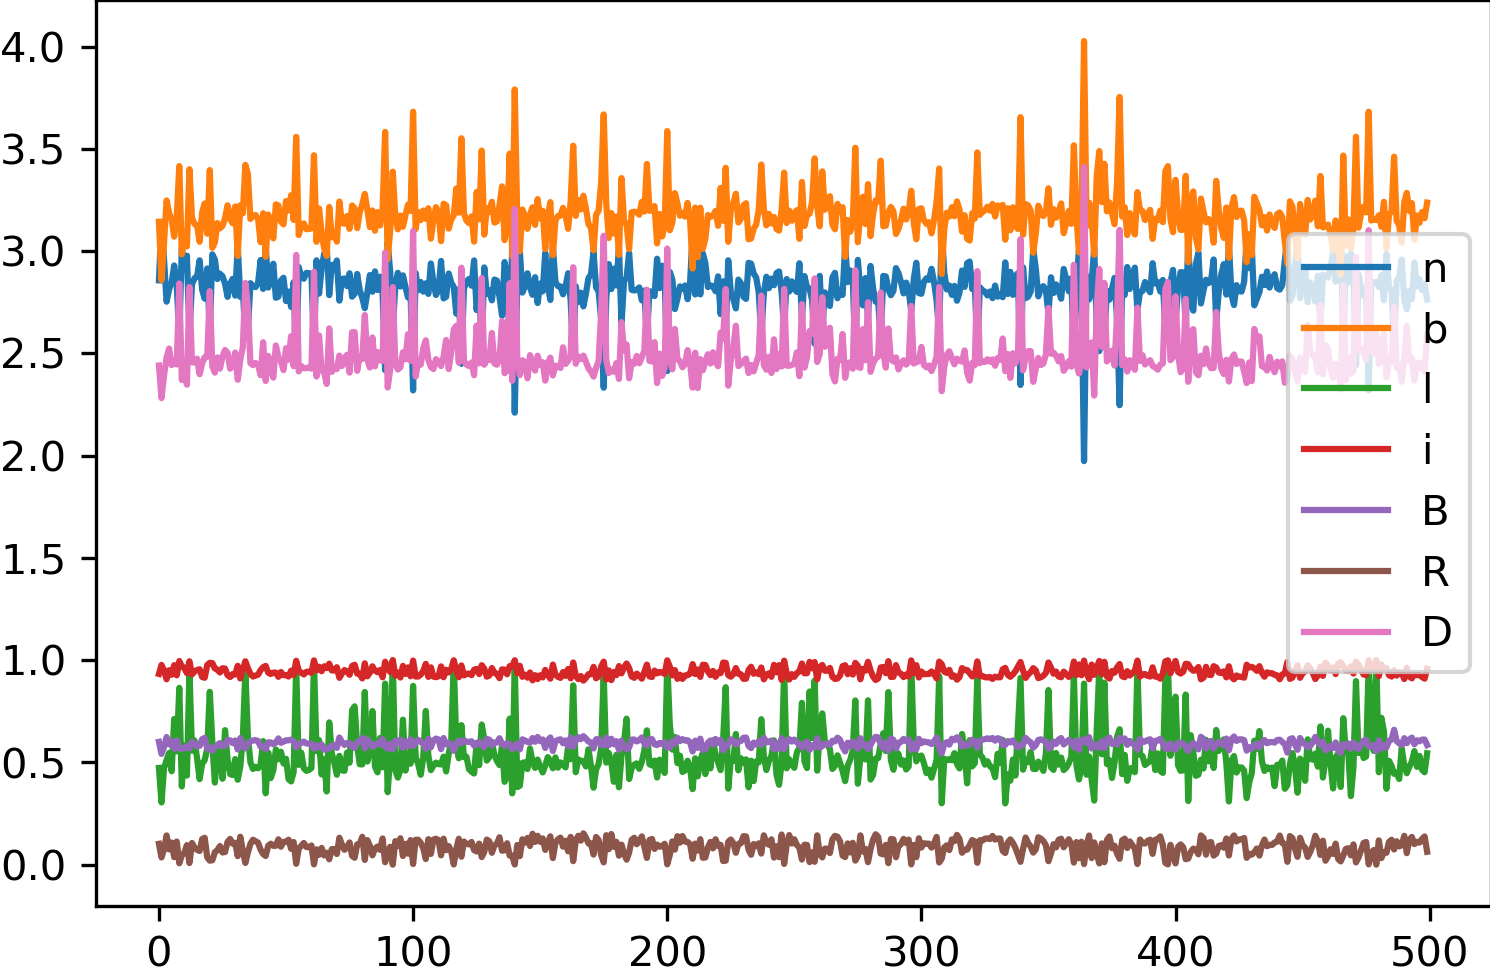
\includegraphics[scale=0.6]{/Graph/500epics.png}
%     \caption{500次随机环境结果}
%     \label{fig:cenAvgTime}
% \end{figure}
% 在不同概率转移和到达速率情况下,各系统参数分布在一定范围内。因此,在之后的实验中,我们在任意给定运维参数下,都将随机运行30次,以均值作为当前参数的结果。以过滤掉系统中骑行因素的影响。

% 为了确定系统参数,我们首先观察研究了随机情况下,单车损坏率与系统状态的关系。如图\ref{fig:betaRate}所示。
% \begin{figure}[H]
%     \centering
%     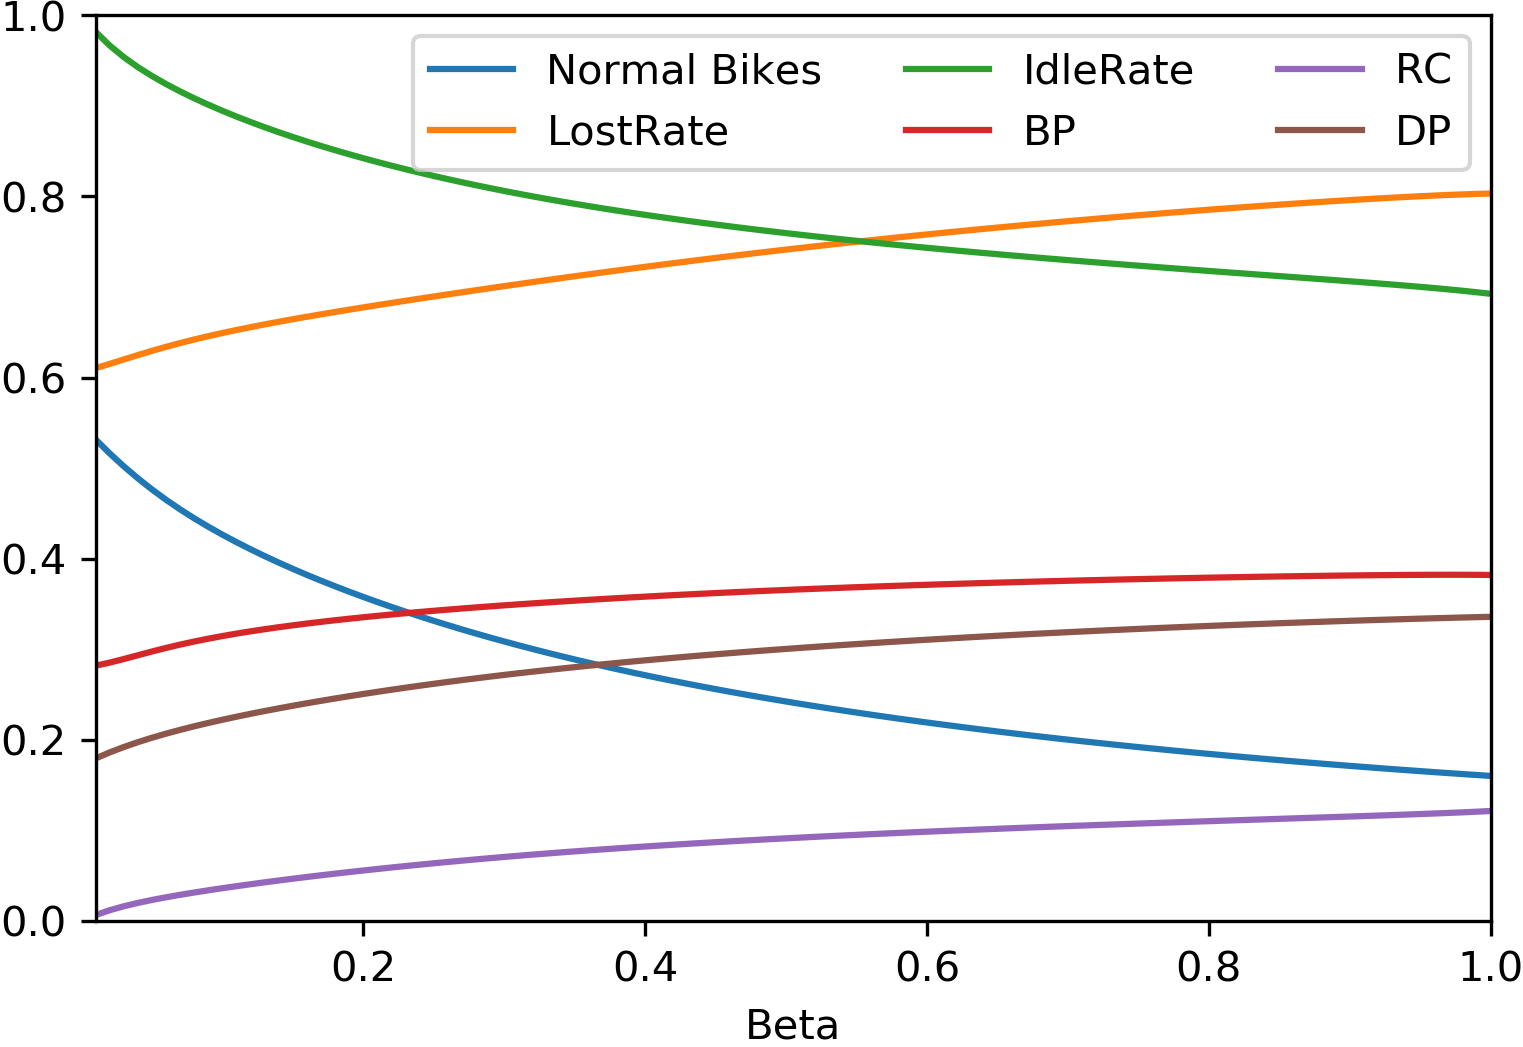
\includegraphics[scale=0.6]{Graph/perfBeta.png}
%     \caption{损坏概率与系统参数变化关系}
%     \label{fig:betaRate}
% \end{figure}
% 随着损坏率的升高系统中好车的比例逐渐下降,顾客的损失比例也会逐渐提高;处在回收、维修和投放过程中的坏车比例升高,维修服务台处在空闲状态的比例逐渐下降。这些现象与常识一致。系统中好车数量下降时,不管系统有怎样的维修能力,在相同的调度安排下,所能服务的顾客数将会减少。同时坏车的数量会增多,处于运维作业过程中的单车比例也会升高。
% 之后,基于给定其他参数的默认值后,进行不同损坏率下系统状态的计算。随着损坏率升高根据观察选取了0.3作为默认值。


% \subsection{实验结果}
% 通过进行数值实验,我们研究共享单车系统中的运维环节对系统整体运行能力的影响。首先我们关注当系统中运维能力有限而要在不同的环节中进行分配的情况。再对各个运维环节的各个参数进行灵敏度分析。在进行数值实验时采用控制变量法。仿真的时间由观察系统进入稳定的时间认为进行确定。

% \subsubsection{运维能力总量有限情况}
% 在实际运营中回收和投放过程是由人工使用运载车搬运完成的。这些人力、车力等通常可以在两项职能中随意切换。因此存在分配的问题。通过在本模型中固定运输速率总和,而变动其中一个,研究系统指标。如图\ref{fig:fixsum}所示。发现当二者相差很大时系统的表现较差。而其余时候表现差异不大。此时提升可分配的总能力,也就是本模型中的二者之和,才可以改善系统表现。但这一改善也存在边际效应递减。同时,提升维修能力也可以一定程度上改善系统的表现。
% $\overline{B}$和$\overline{D}$对系统的影响是相似的。稳态计算和仿真都显示当$\overline{B}$和$\overline{D}$相近时,系统中好车的比例较高。他们对系统性能指标的影响是非单调的,在仿真的结果中可以观察到,系统的表现最初随着批量的升高有所改善,到达某一峰值后开始下降。因此在实践中需要结合经验确定合理的回收批量。
% %\newgeometry{left=0.1cm,right=0.1cm, top=0.1cm, bottom=0.1cm}
% \begin{figure}[H]
%     \centering
%     \subfigure[回收与投放速度总和为定值,变动总和]{
%     \begin{minipage}[t]{0.5\textwidth}
%     \centering
%     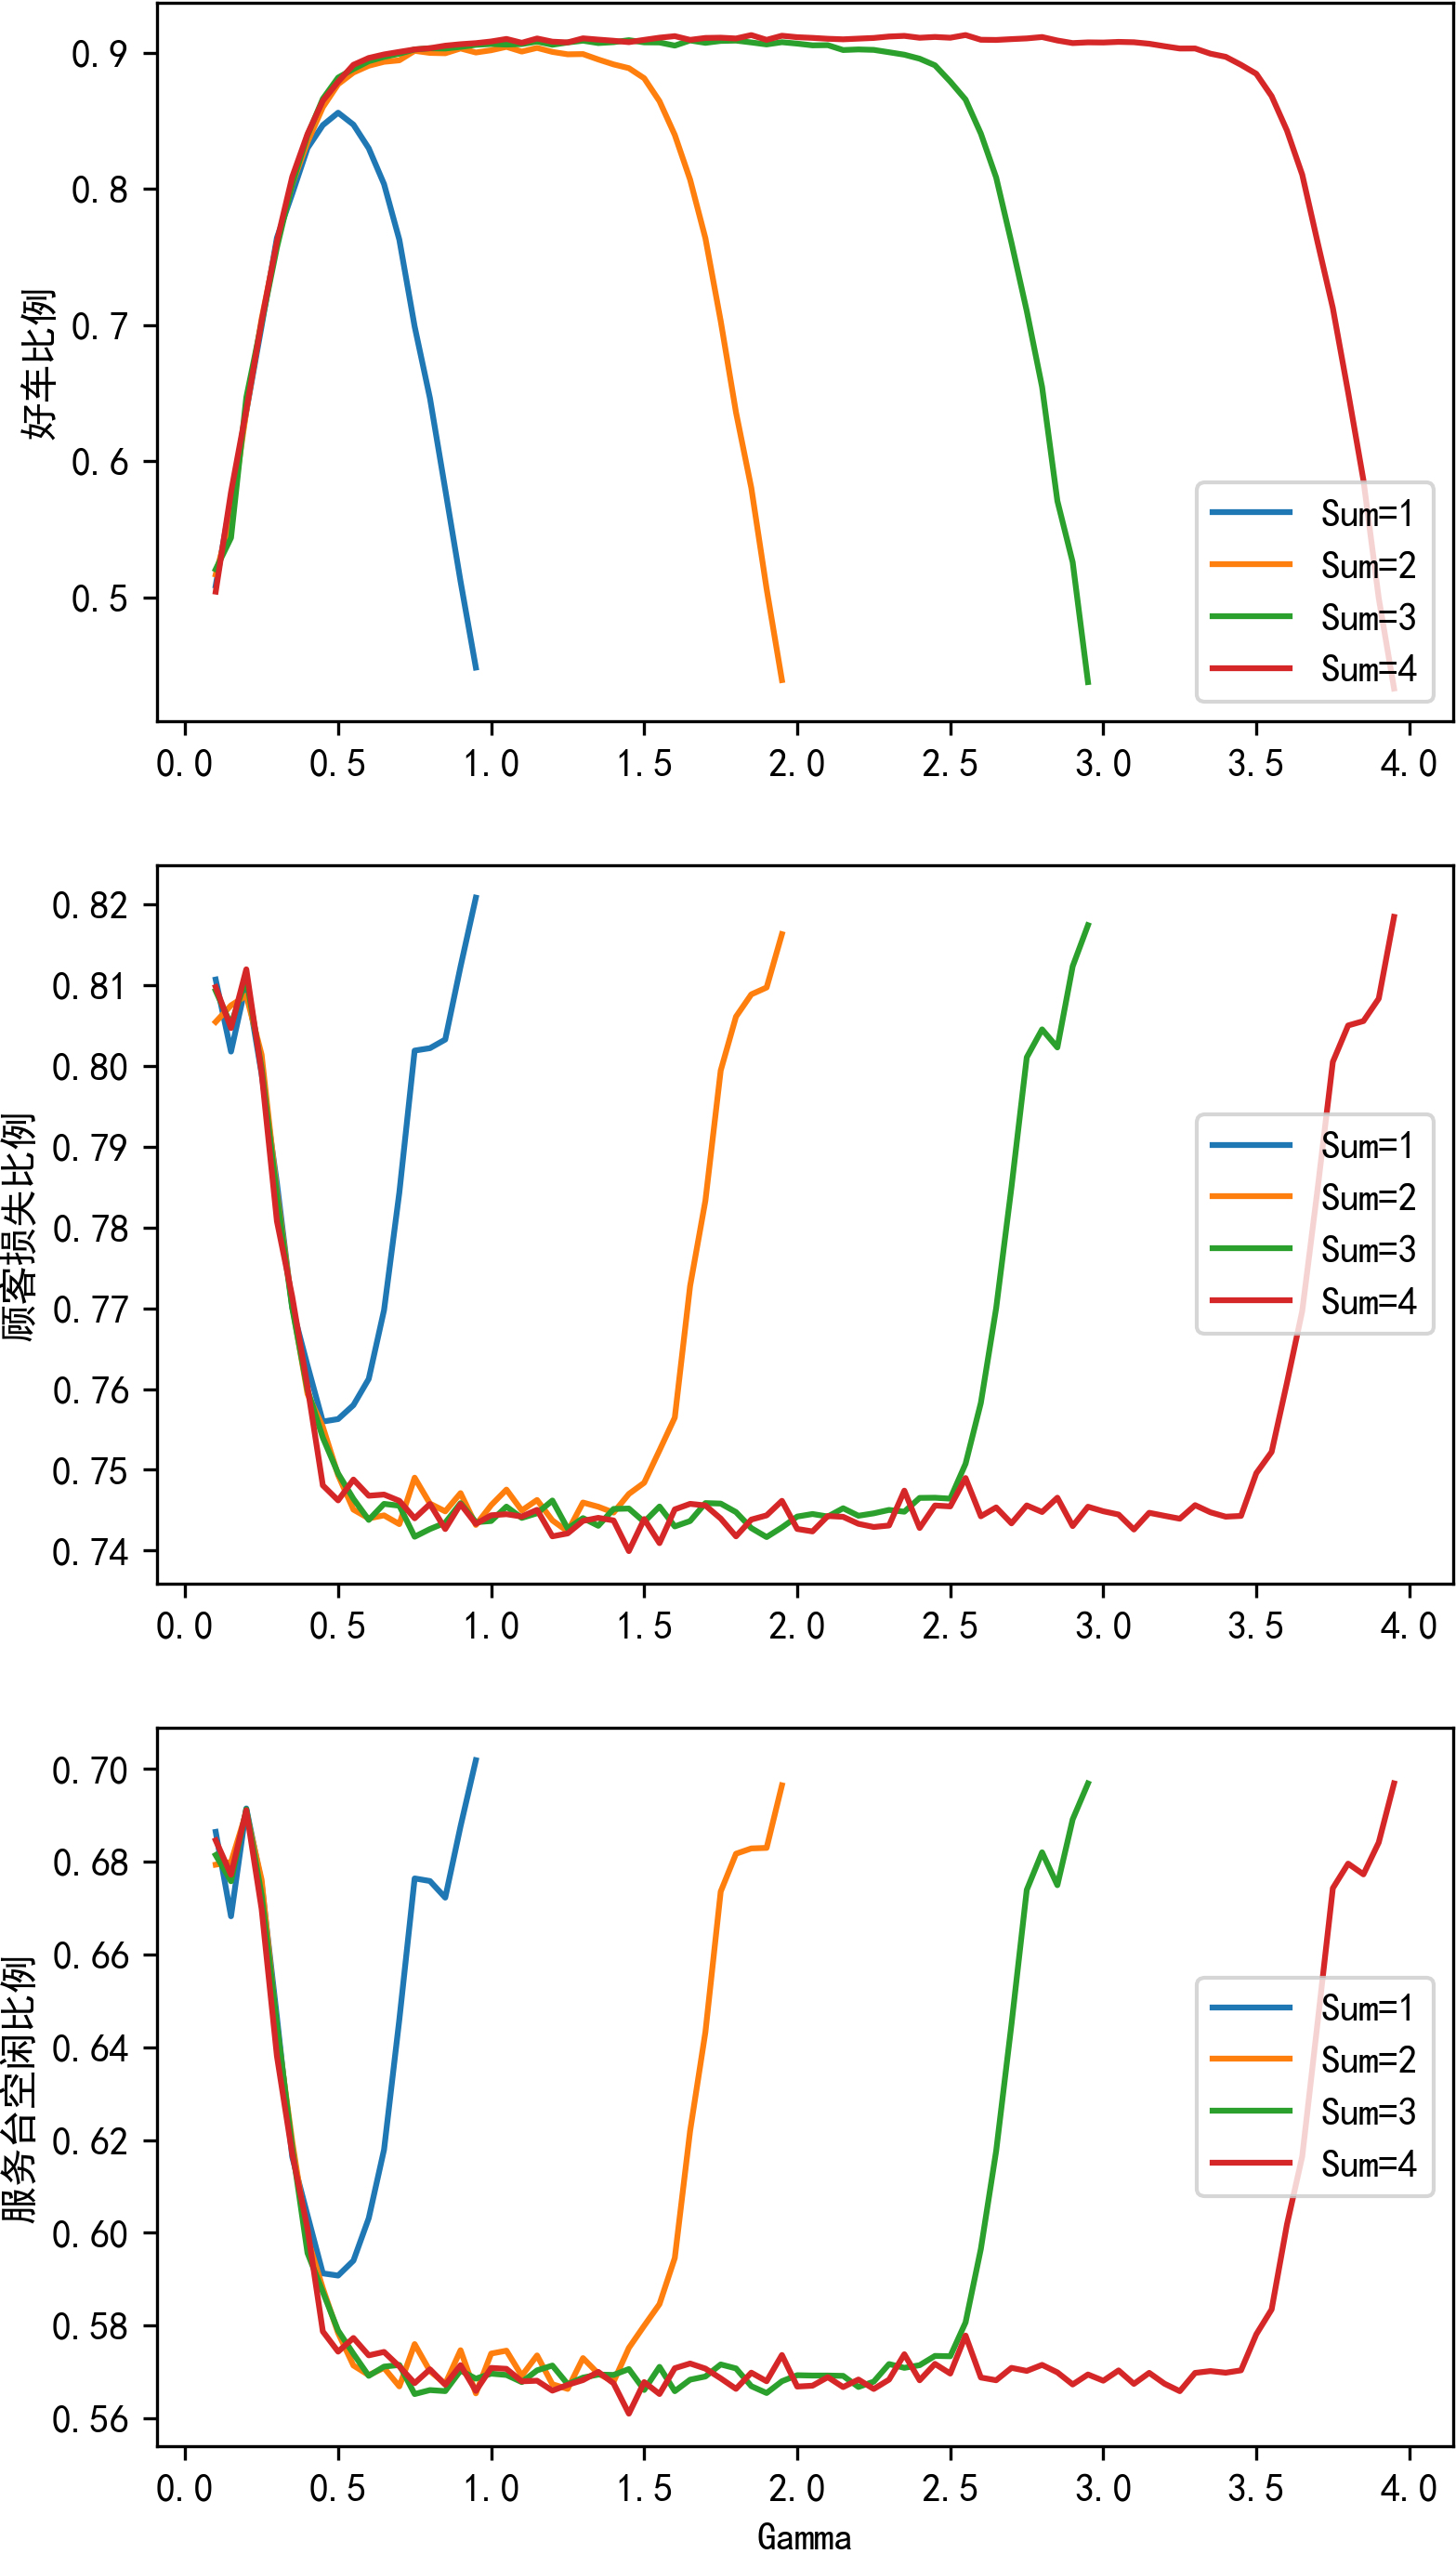
\includegraphics[width=2.4in]{Graph/perf/perfA10M50DeltaGammaSumVaryMu.png}
%     %\caption{fig2}
%     \end{minipage}%
%     }%
%     \centering
%     \subfigure[回收与投放速度总和为定值,变动维修速率]{
%     \begin{minipage}[t]{0.5\textwidth}
%     \centering
%     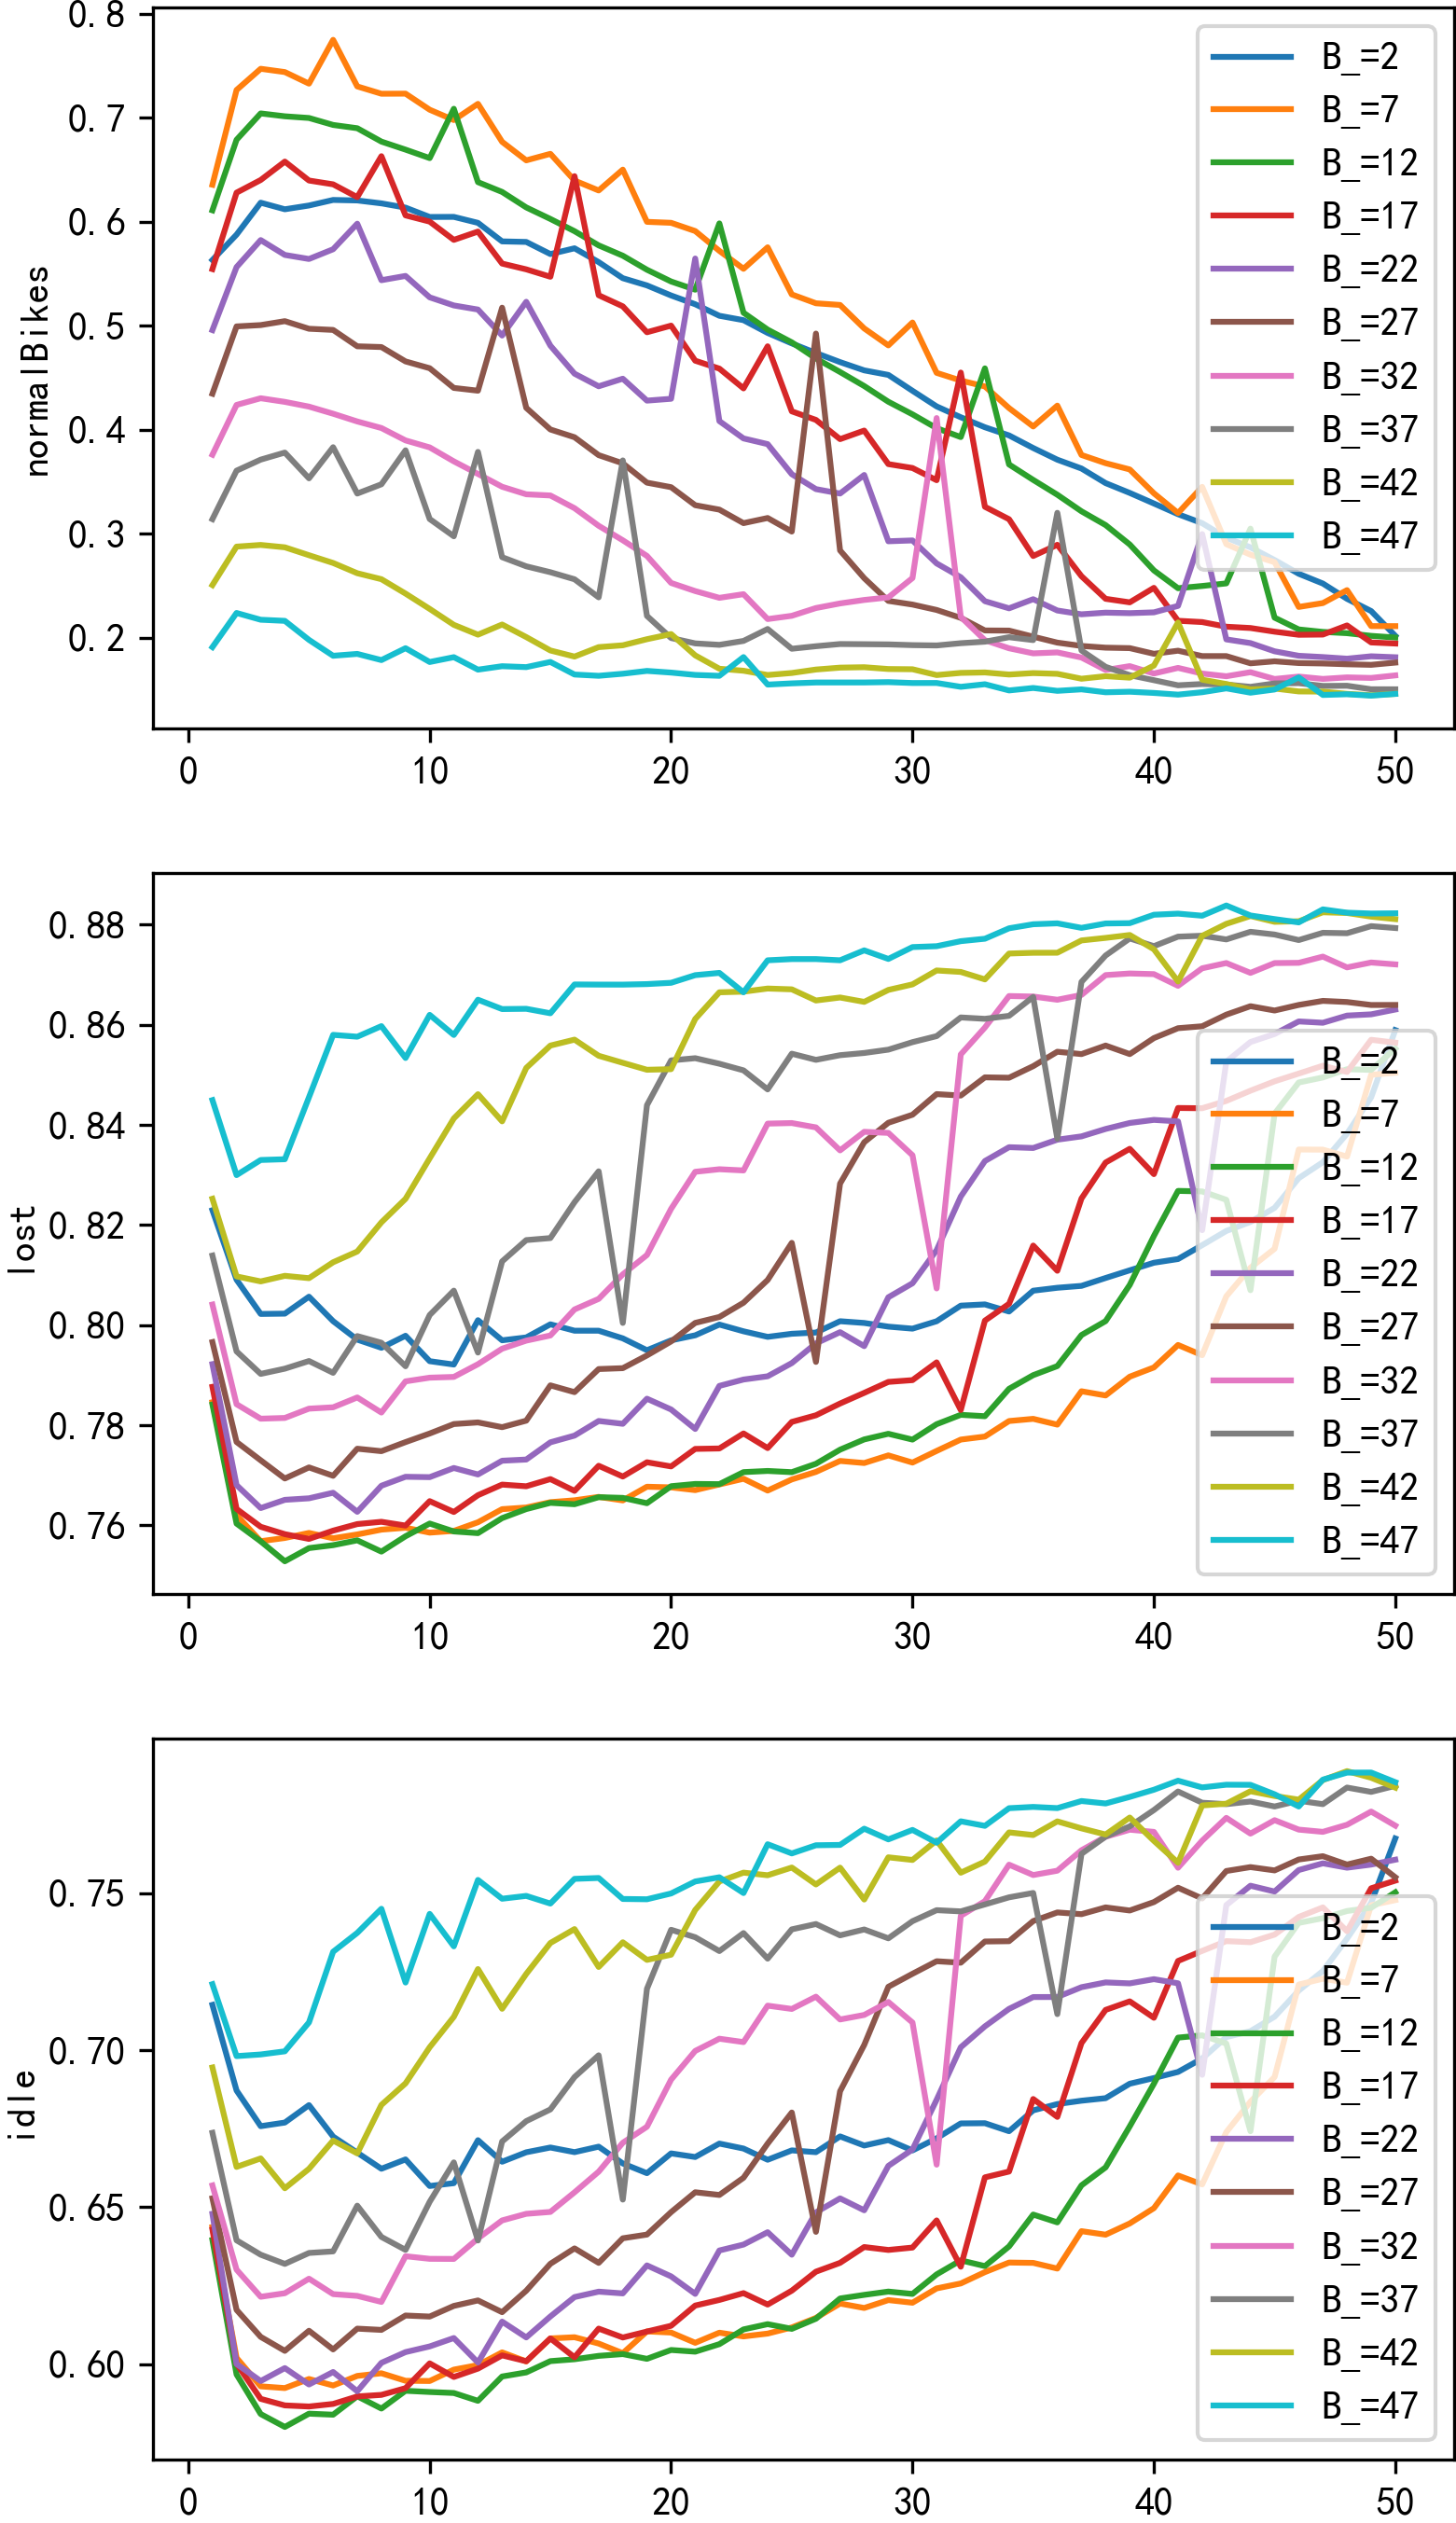
\includegraphics[width=2.3in]{Graph/perf/perfA10M50B_-D_.png}
%     %\caption{fig1}
%     \end{minipage}%
%     }%xs
%     \caption{运维能力总量有限情况}
%     \label{fig:fixsum}
% \end{figure}
% %\restoregeometry

% % \begin{figure}[htbp]

% %     \centering
    
% %     \subfloat[回收与投放速度总和为定值,变动总和]{
    
% %     \label{fig:improved_subfig_a}
    
% %     \begin{minipage}[t]{0.3\textwidth}
    
% %     \centering
    
% %     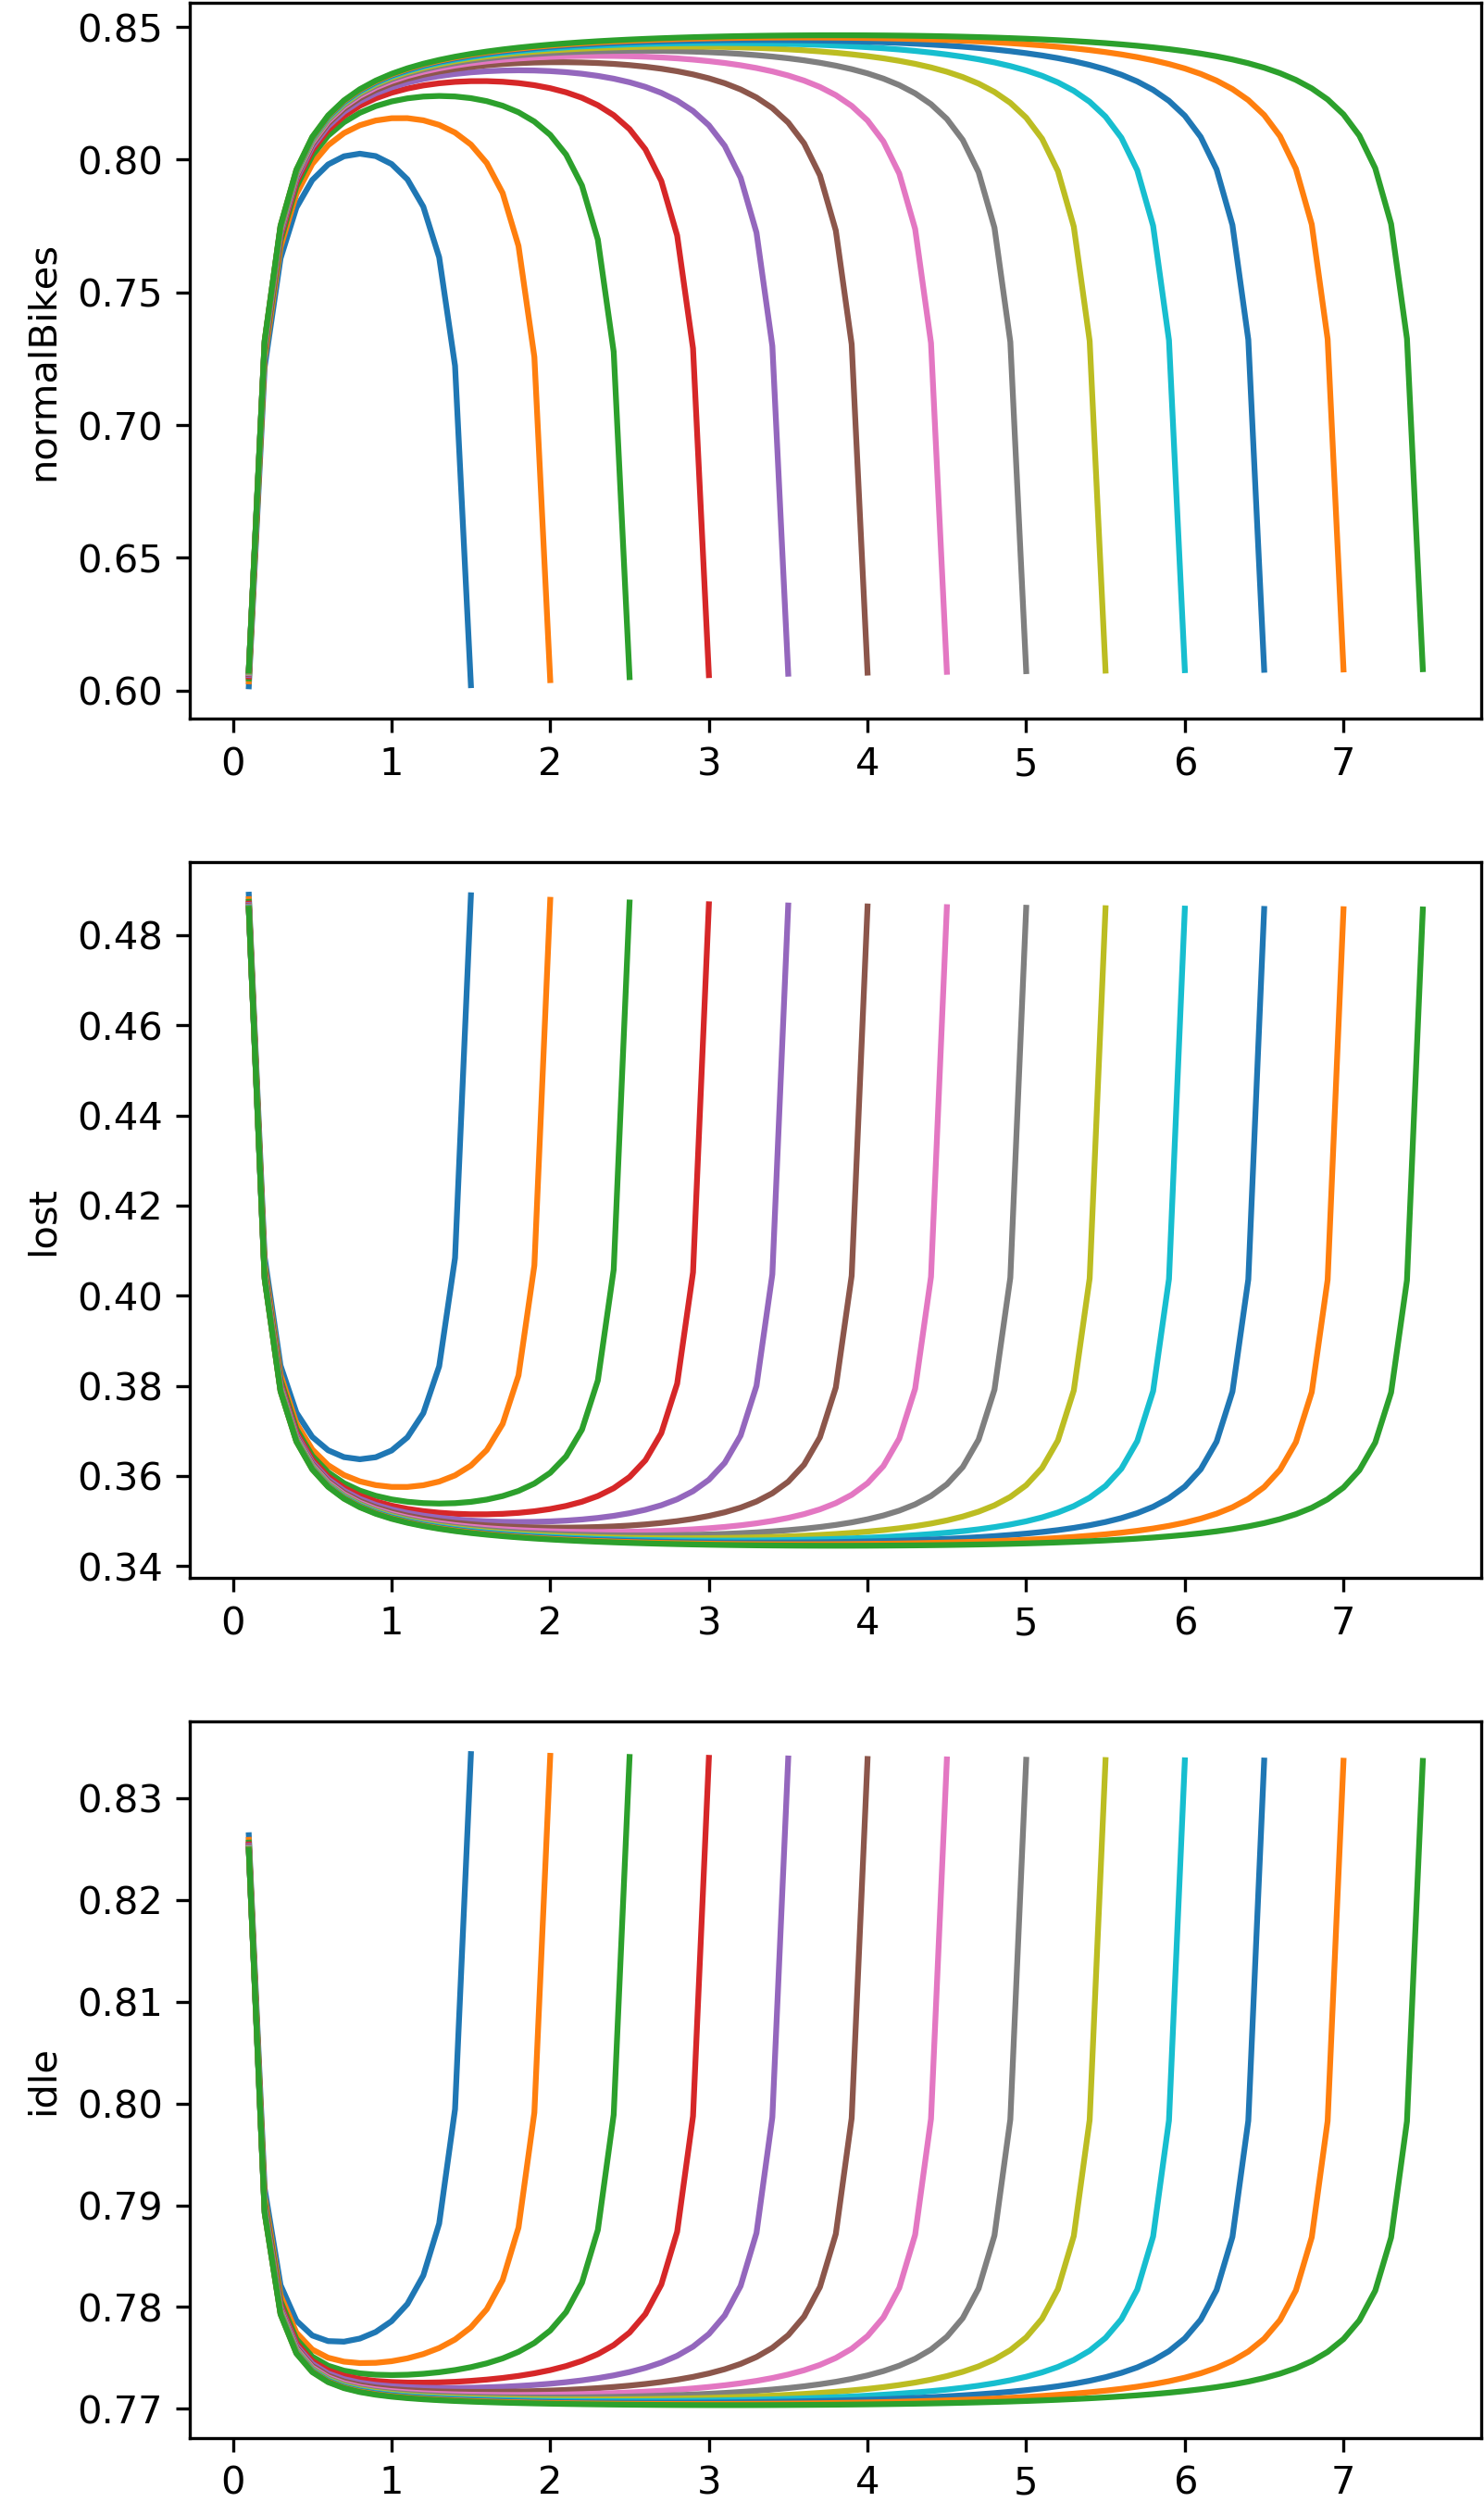
\includegraphics[width=2.4in]{Graph/perf/perfGamma+Delta0-Sum0-8lines.png}
    
% %     \end{minipage}
    
% %     }
    
% %     \subfloat[回收与投放速度总和为定值,变动维修速率]{
    
% %     \label{fig:improved_subfig_b}
    
% %     \begin{minipage}[t]{0.3\textwidth}
    
% %     \centering
    
% %     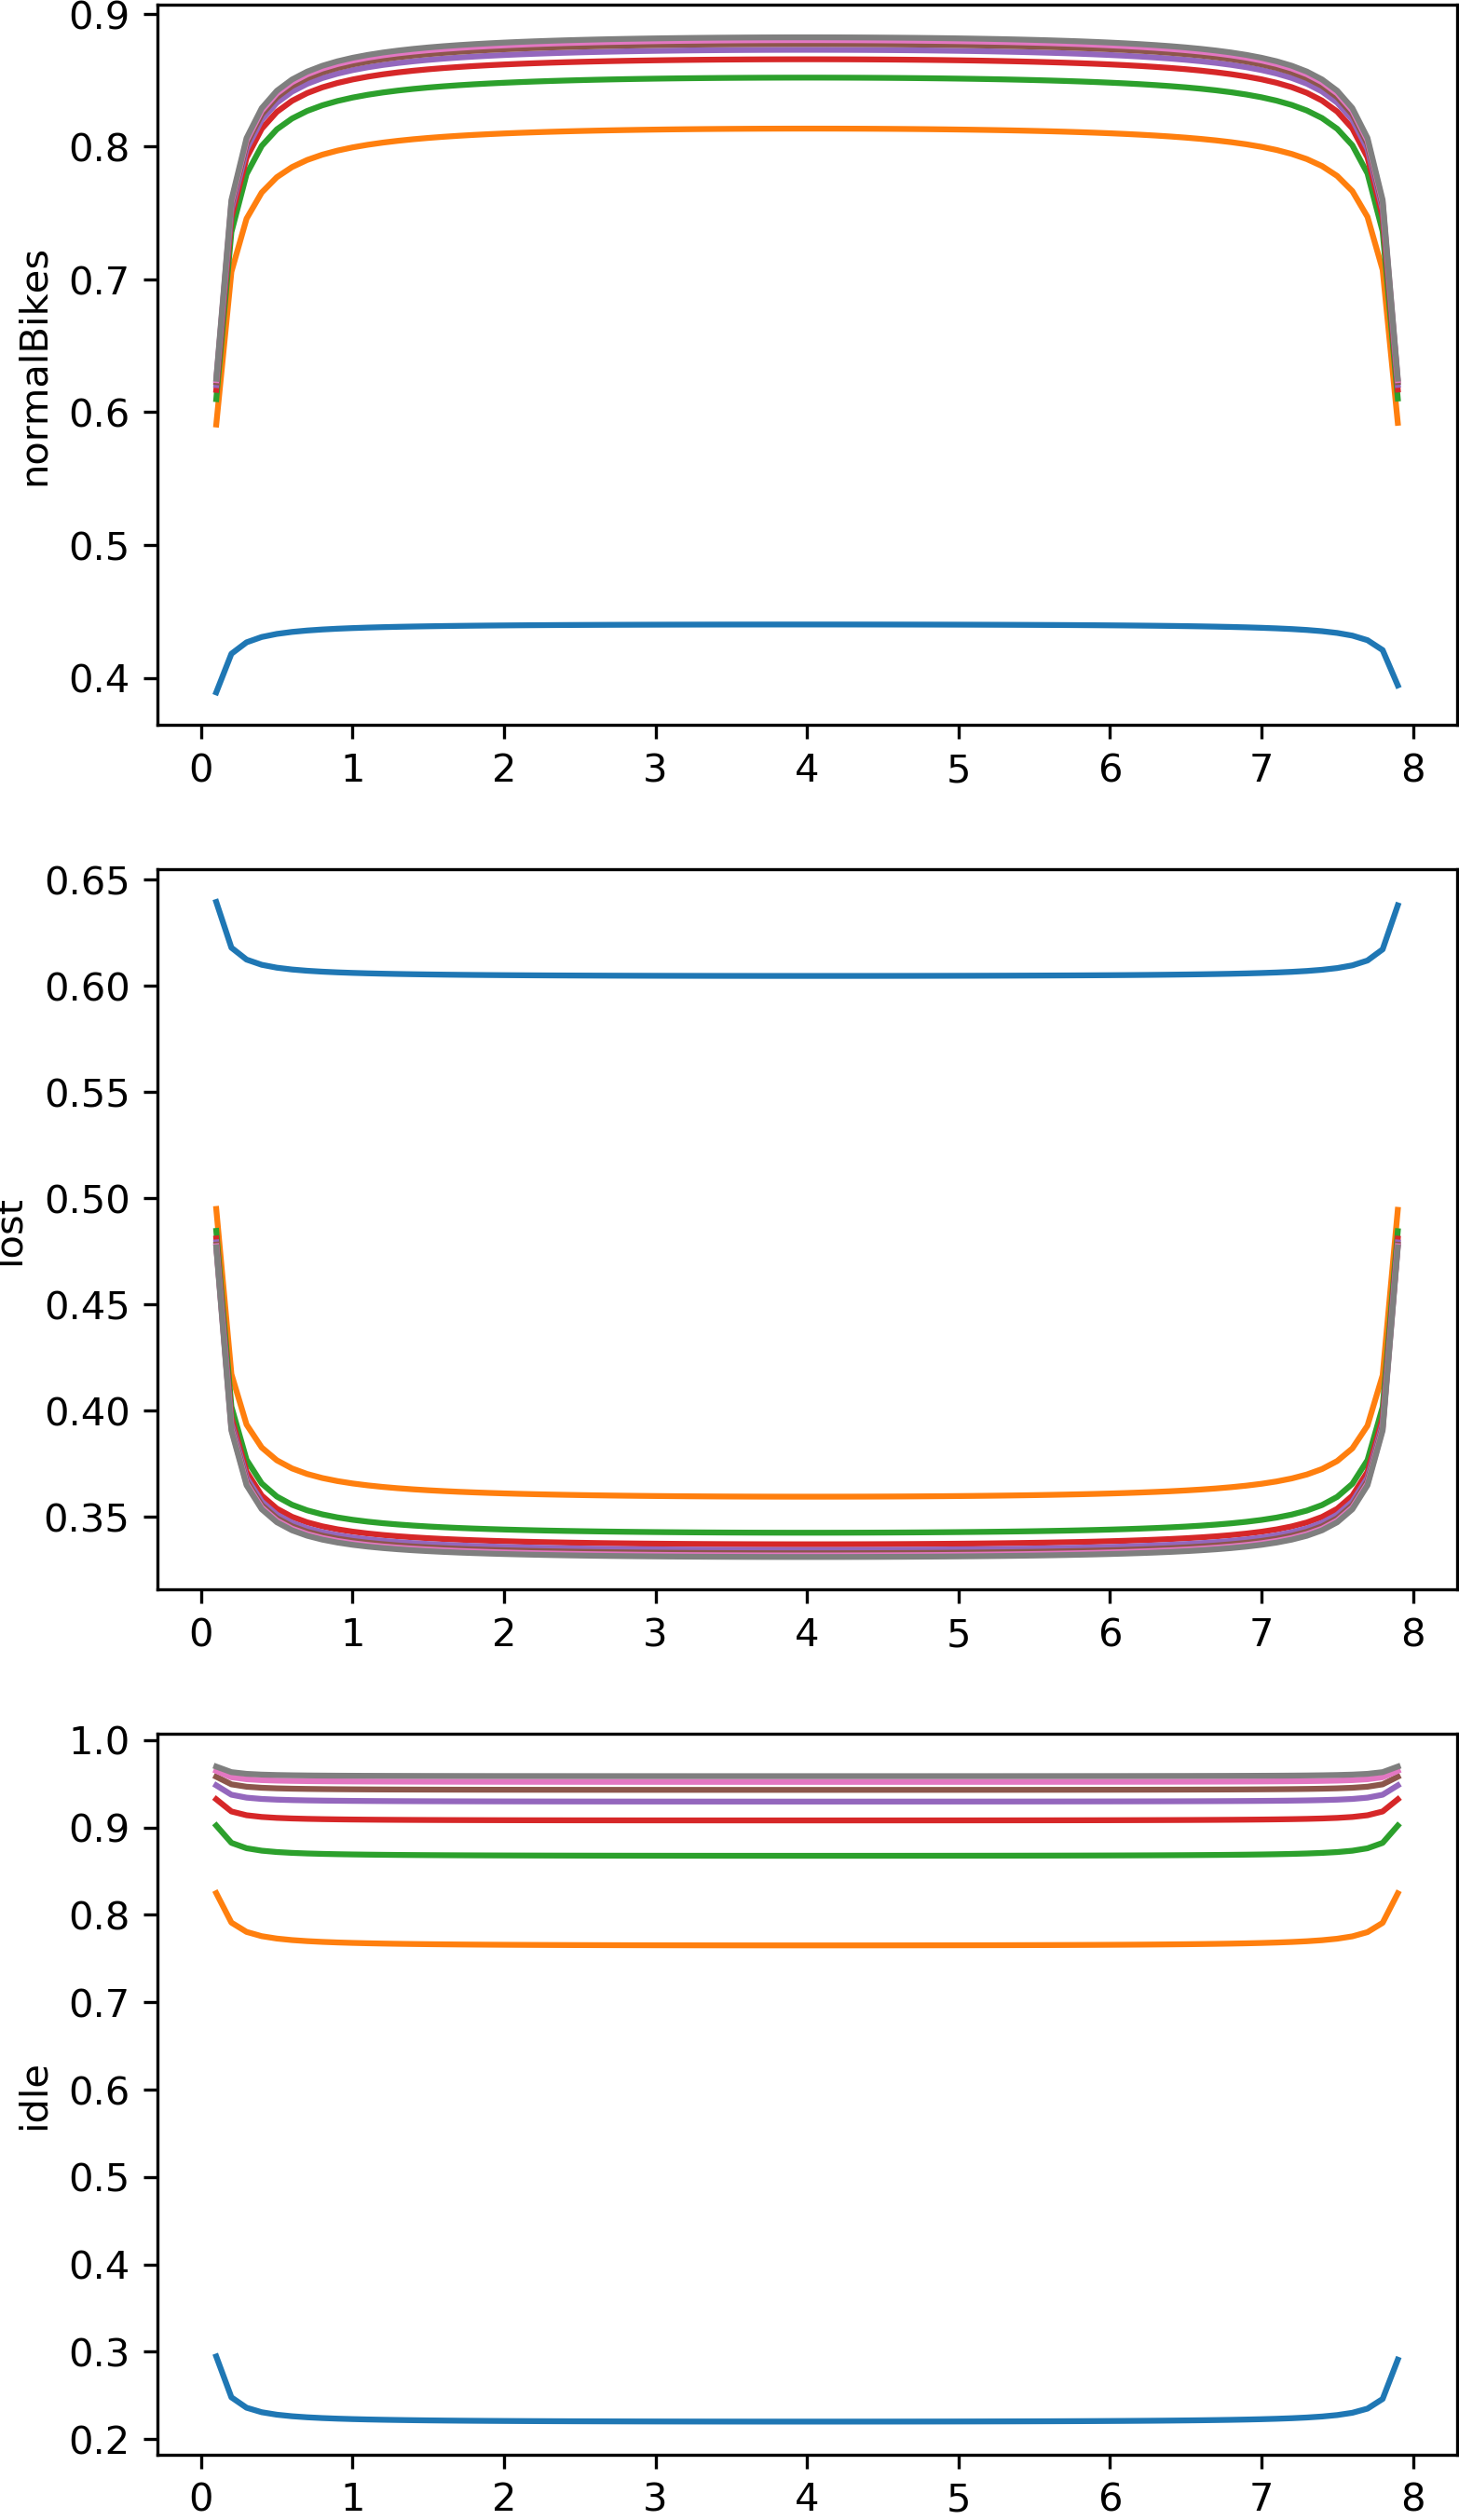
\includegraphics[width=2.3in]{Graph/perf/perfGamma+Delta0-8Mu0-4-8lines.png}
    
% %     \end{minipage}
    
% %     }
    
% %     \caption{运维能力总量有限情况}
% %     \label{fig:fixsum}
    
% %     \end{figure}

% \subsubsection{灵敏度分析}
% 本部分分析某服务环节参数变化对系统运行状态的影响。
% 改善每个环节都可以提升系统,但是有瓶颈。边际效应递减。回收和投放的效果接近。
% 单独提升回收、维修和投放速率能够增大系统中好车的比例,减少客户的损失。改善的效果逐渐减弱,直至不再起作用。
% 回收和投放批量与系统中的好车数和顾客损失率呈阶梯函数关系。总体来说这二者的增大,不利于系统的服务能力的提升。但一定程度的改变不影响系统能力,因此在实际场景中可以通过经验,确定合适的运输批量。

% %\newgeometry{left=0.1cm,right=0.1cm, top=0.1cm, bottom=0.1cm}
% \begin{figure}[H]
%     \centering
%     \subfigure[$\overline{B}$-Gamma]{
%     \begin{minipage}[t]{0.5\linewidth}
%     \centering
%     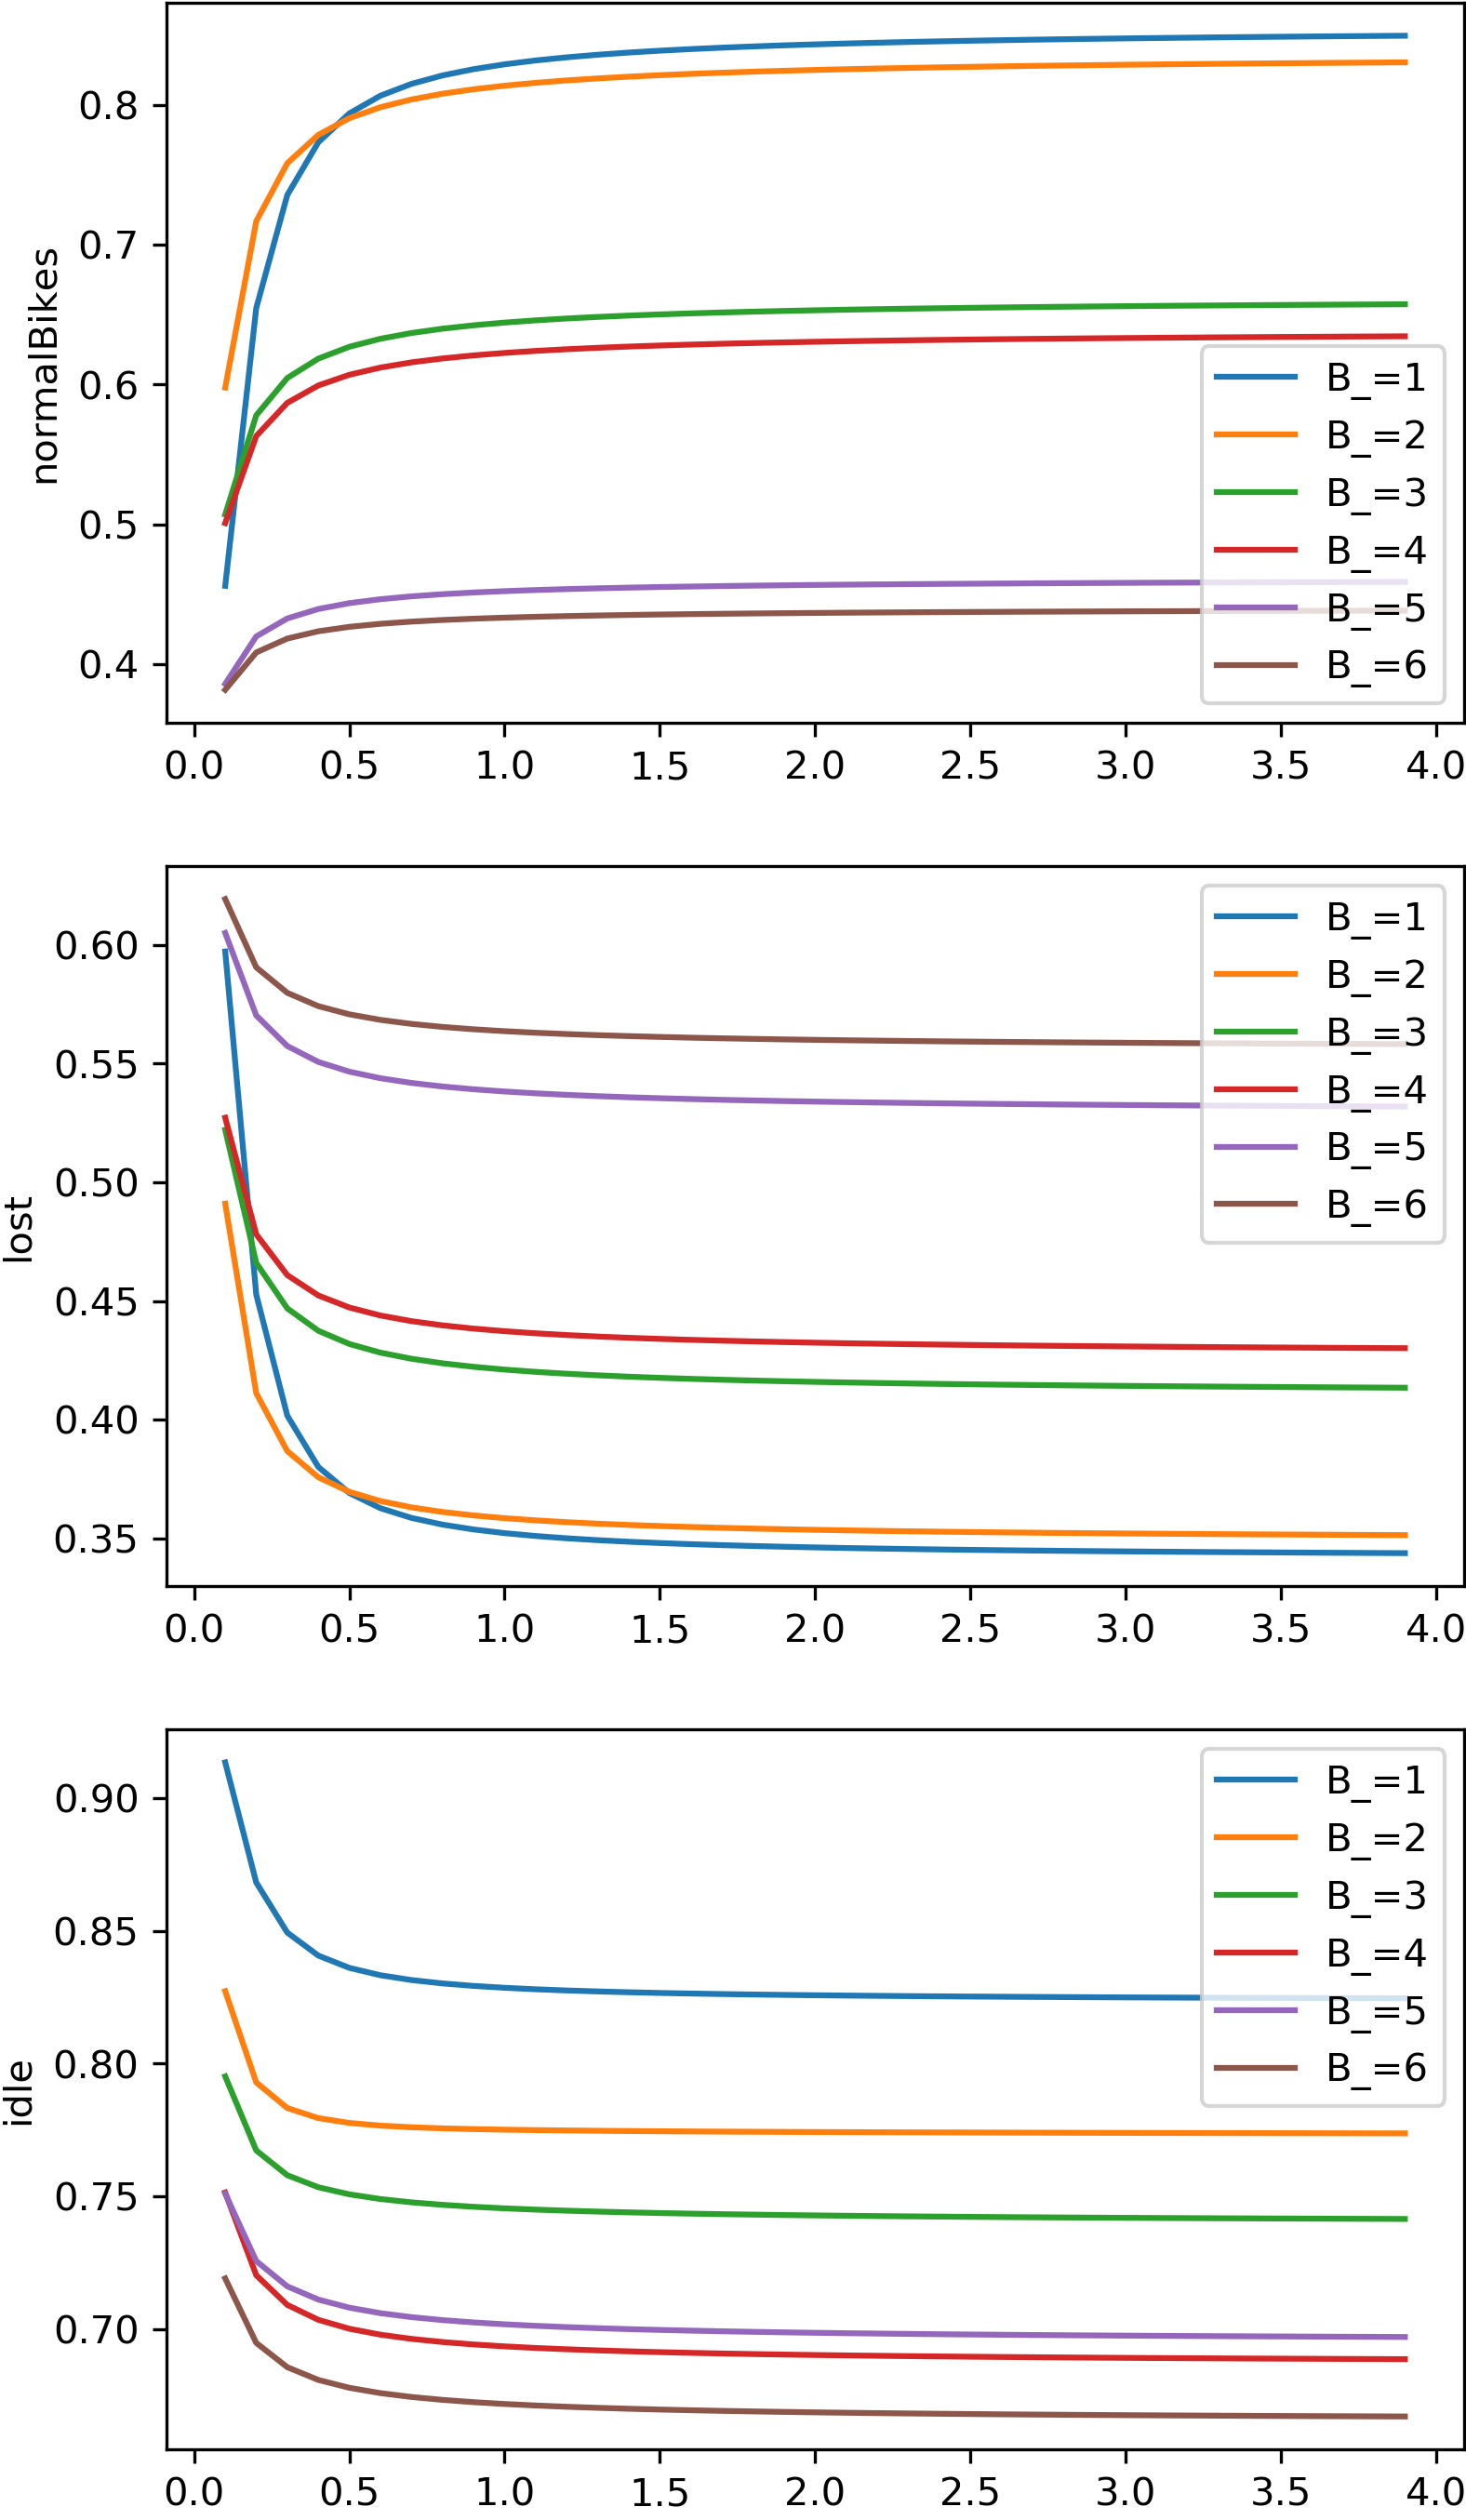
\includegraphics[width=2.25in]{Graph/perf/perfB_1-6Gamma0-4.png}
%     %\caption{fig1}
%     \end{minipage}%
%     }%
%     \centering
%     \subfigure[N-Mu]{
%     \begin{minipage}[t]{0.5\linewidth}
%     \centering
%     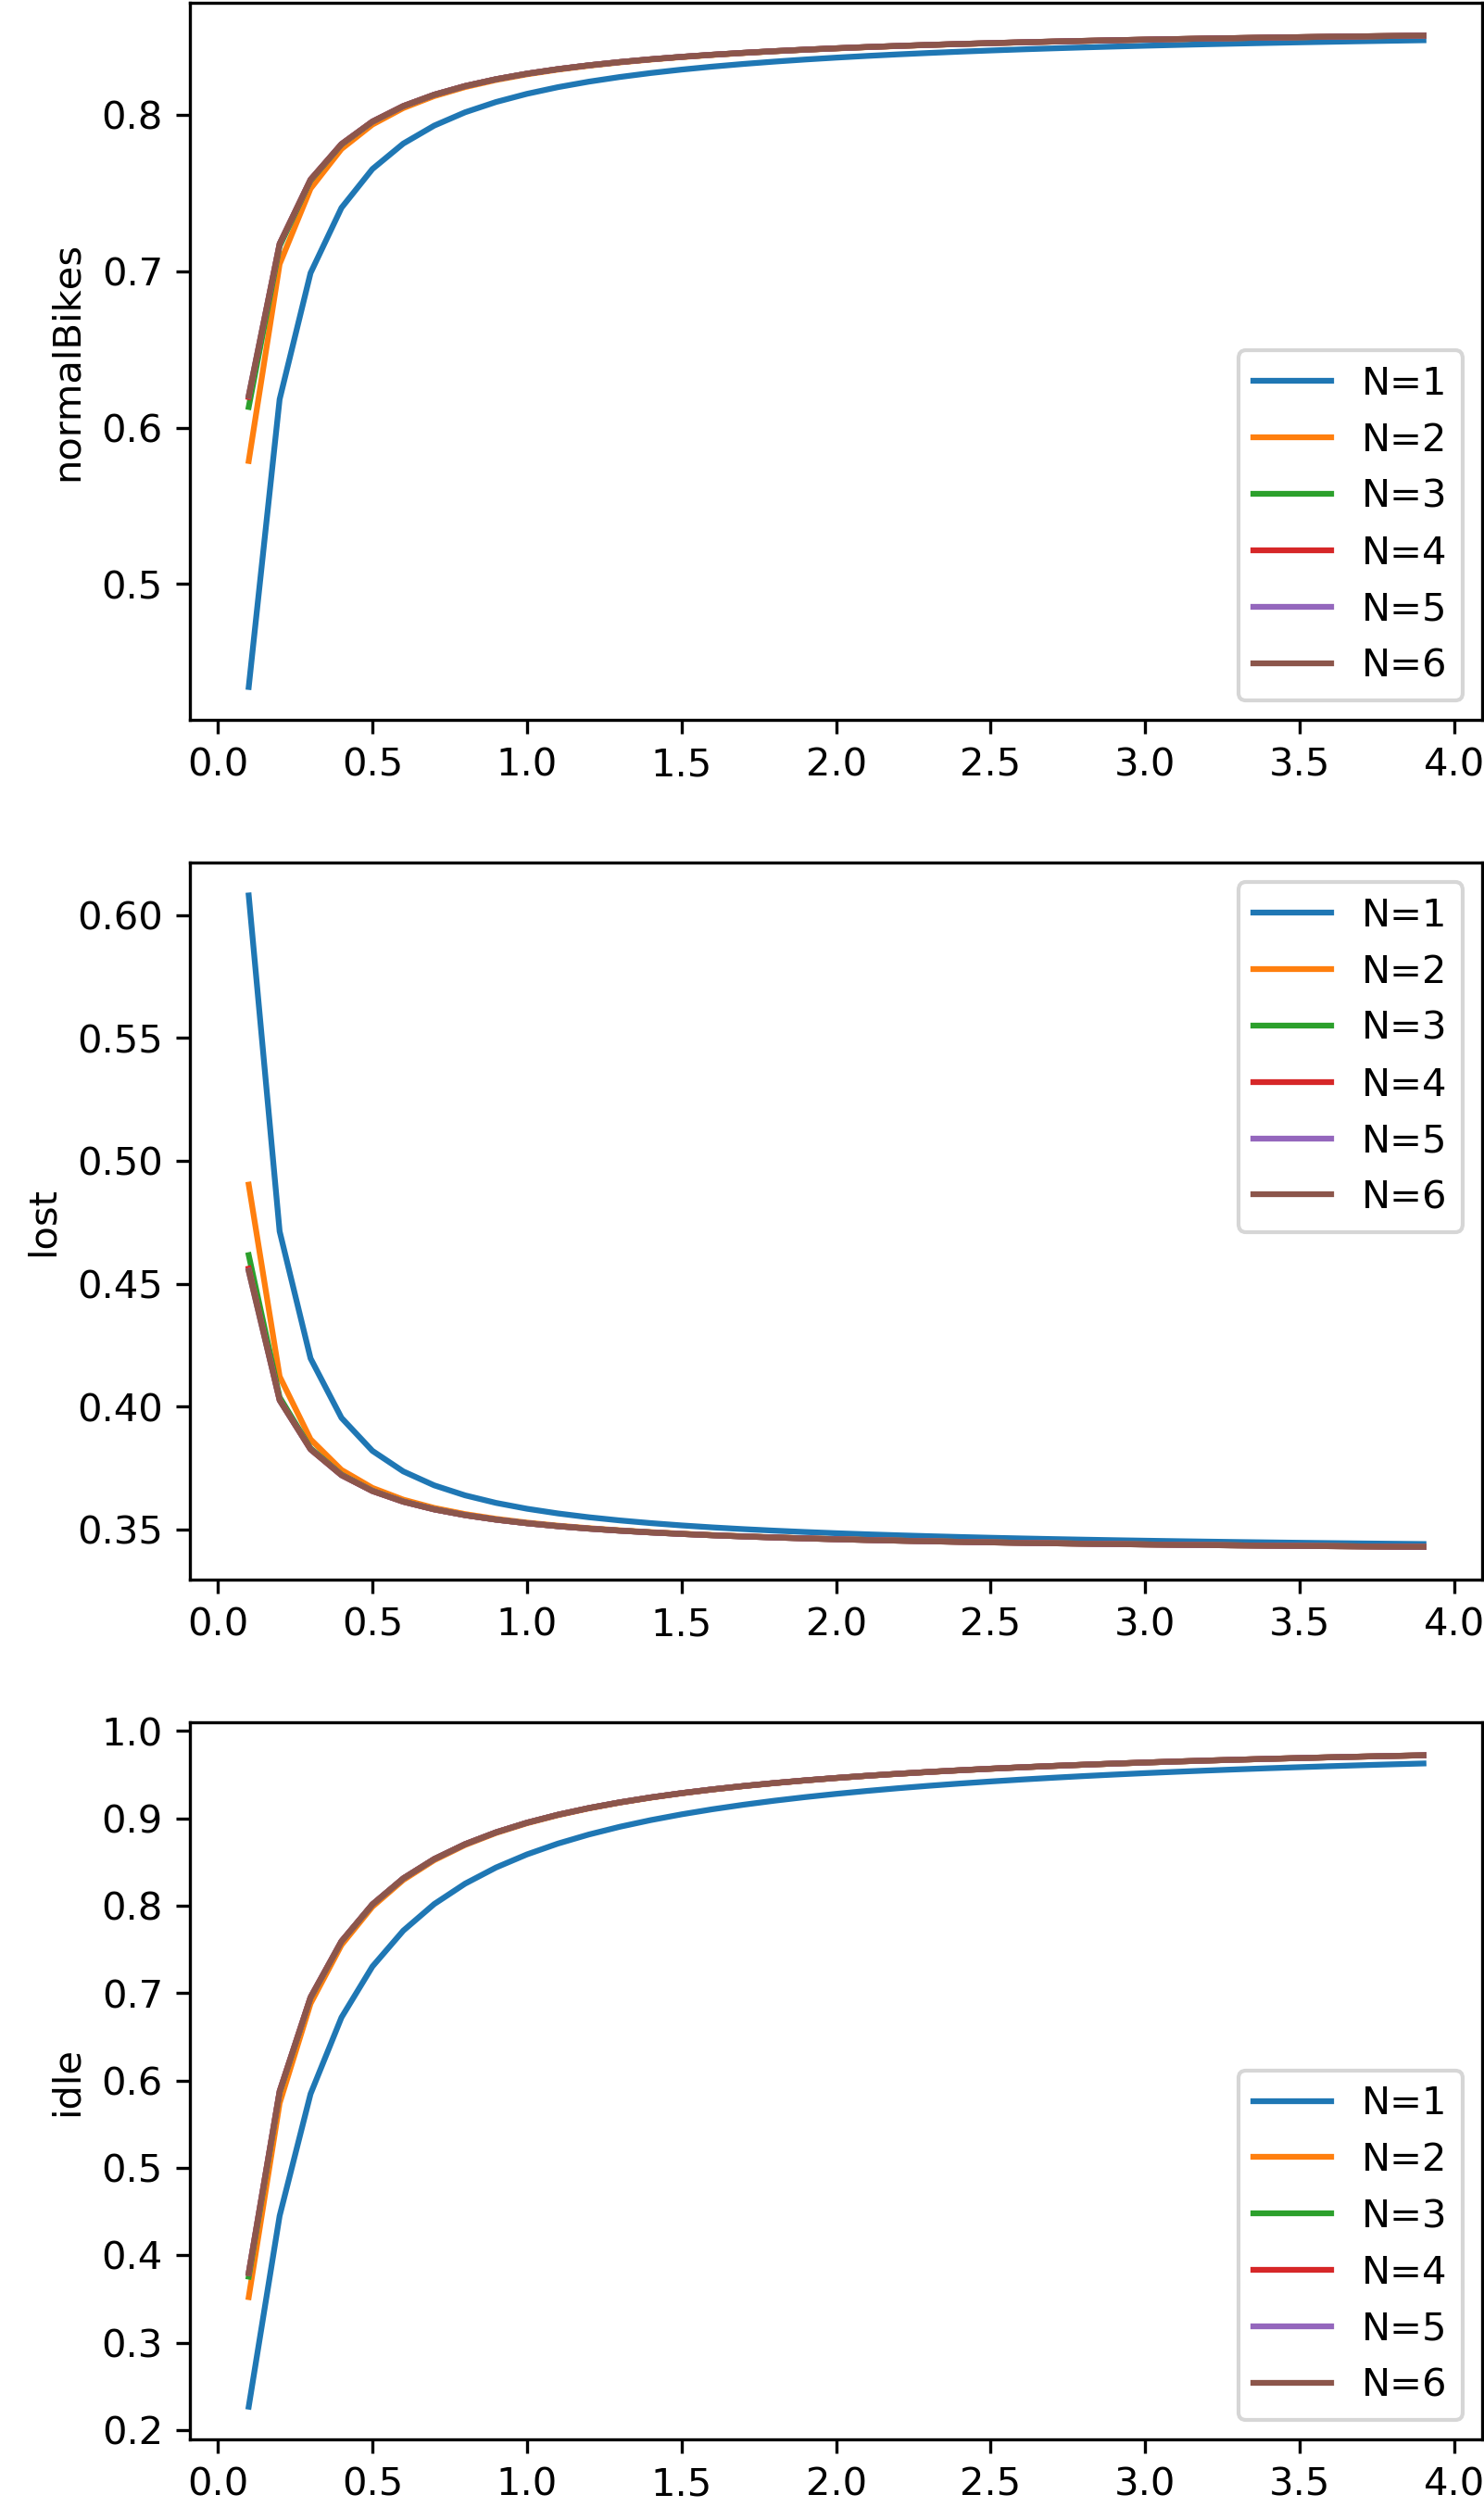
\includegraphics[width=2.3in]{Graph/perf/perfNMu.png}
%     %\caption{fig2}
%     \end{minipage}%
%     }%
% \end{figure}
% %\restoregeometry

% %\newgeometry{left=0.1cm,right=0.1cm, top=0.1cm, bottom=0.1cm}
% \begin{figure}[H]
%     \centering
%     \subfigure[$\overline{D}$-Delta]{
%     \begin{minipage}[t]{0.5\linewidth}
%     \centering
%     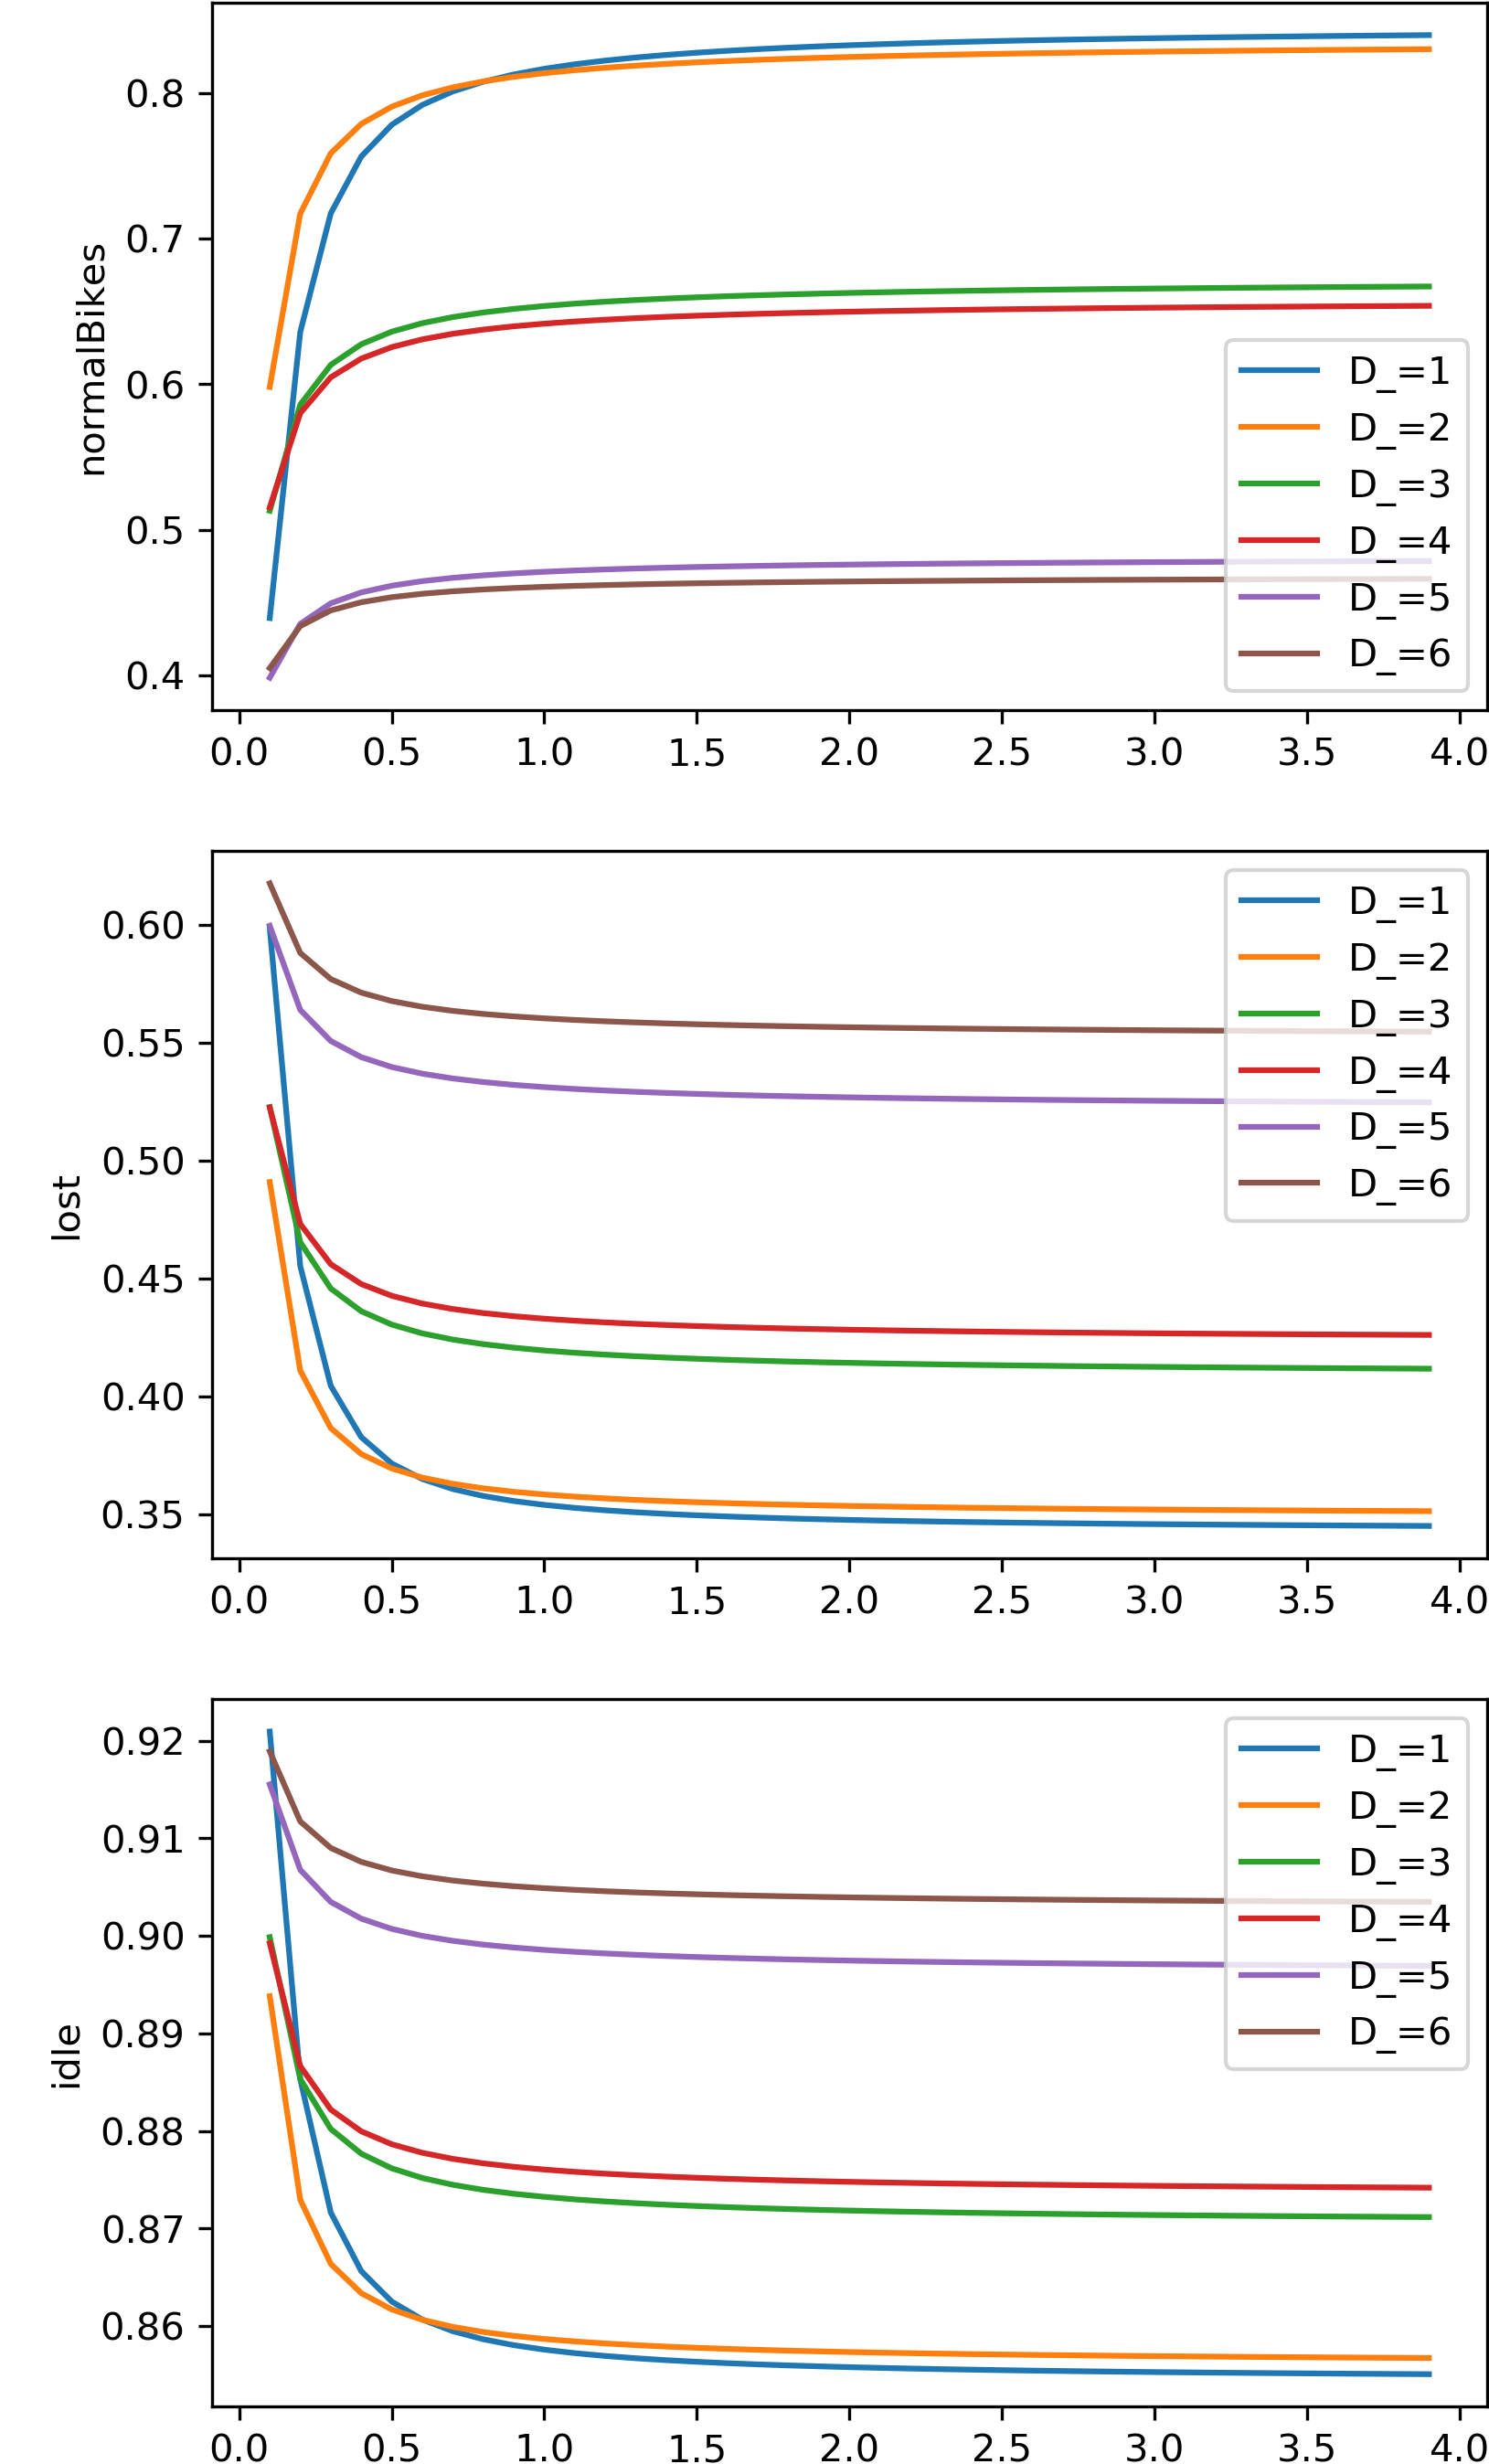
\includegraphics[width=2.4in]{Graph/perf/perfD_Delta.png}
%     %\caption{fig2}
%     \end{minipage}%
%     }%
%     \centering
%     \subfigure[$\overline{B}-\overline{D}$]{
%     \begin{minipage}[t]{0.5\linewidth}
%     \centering
%     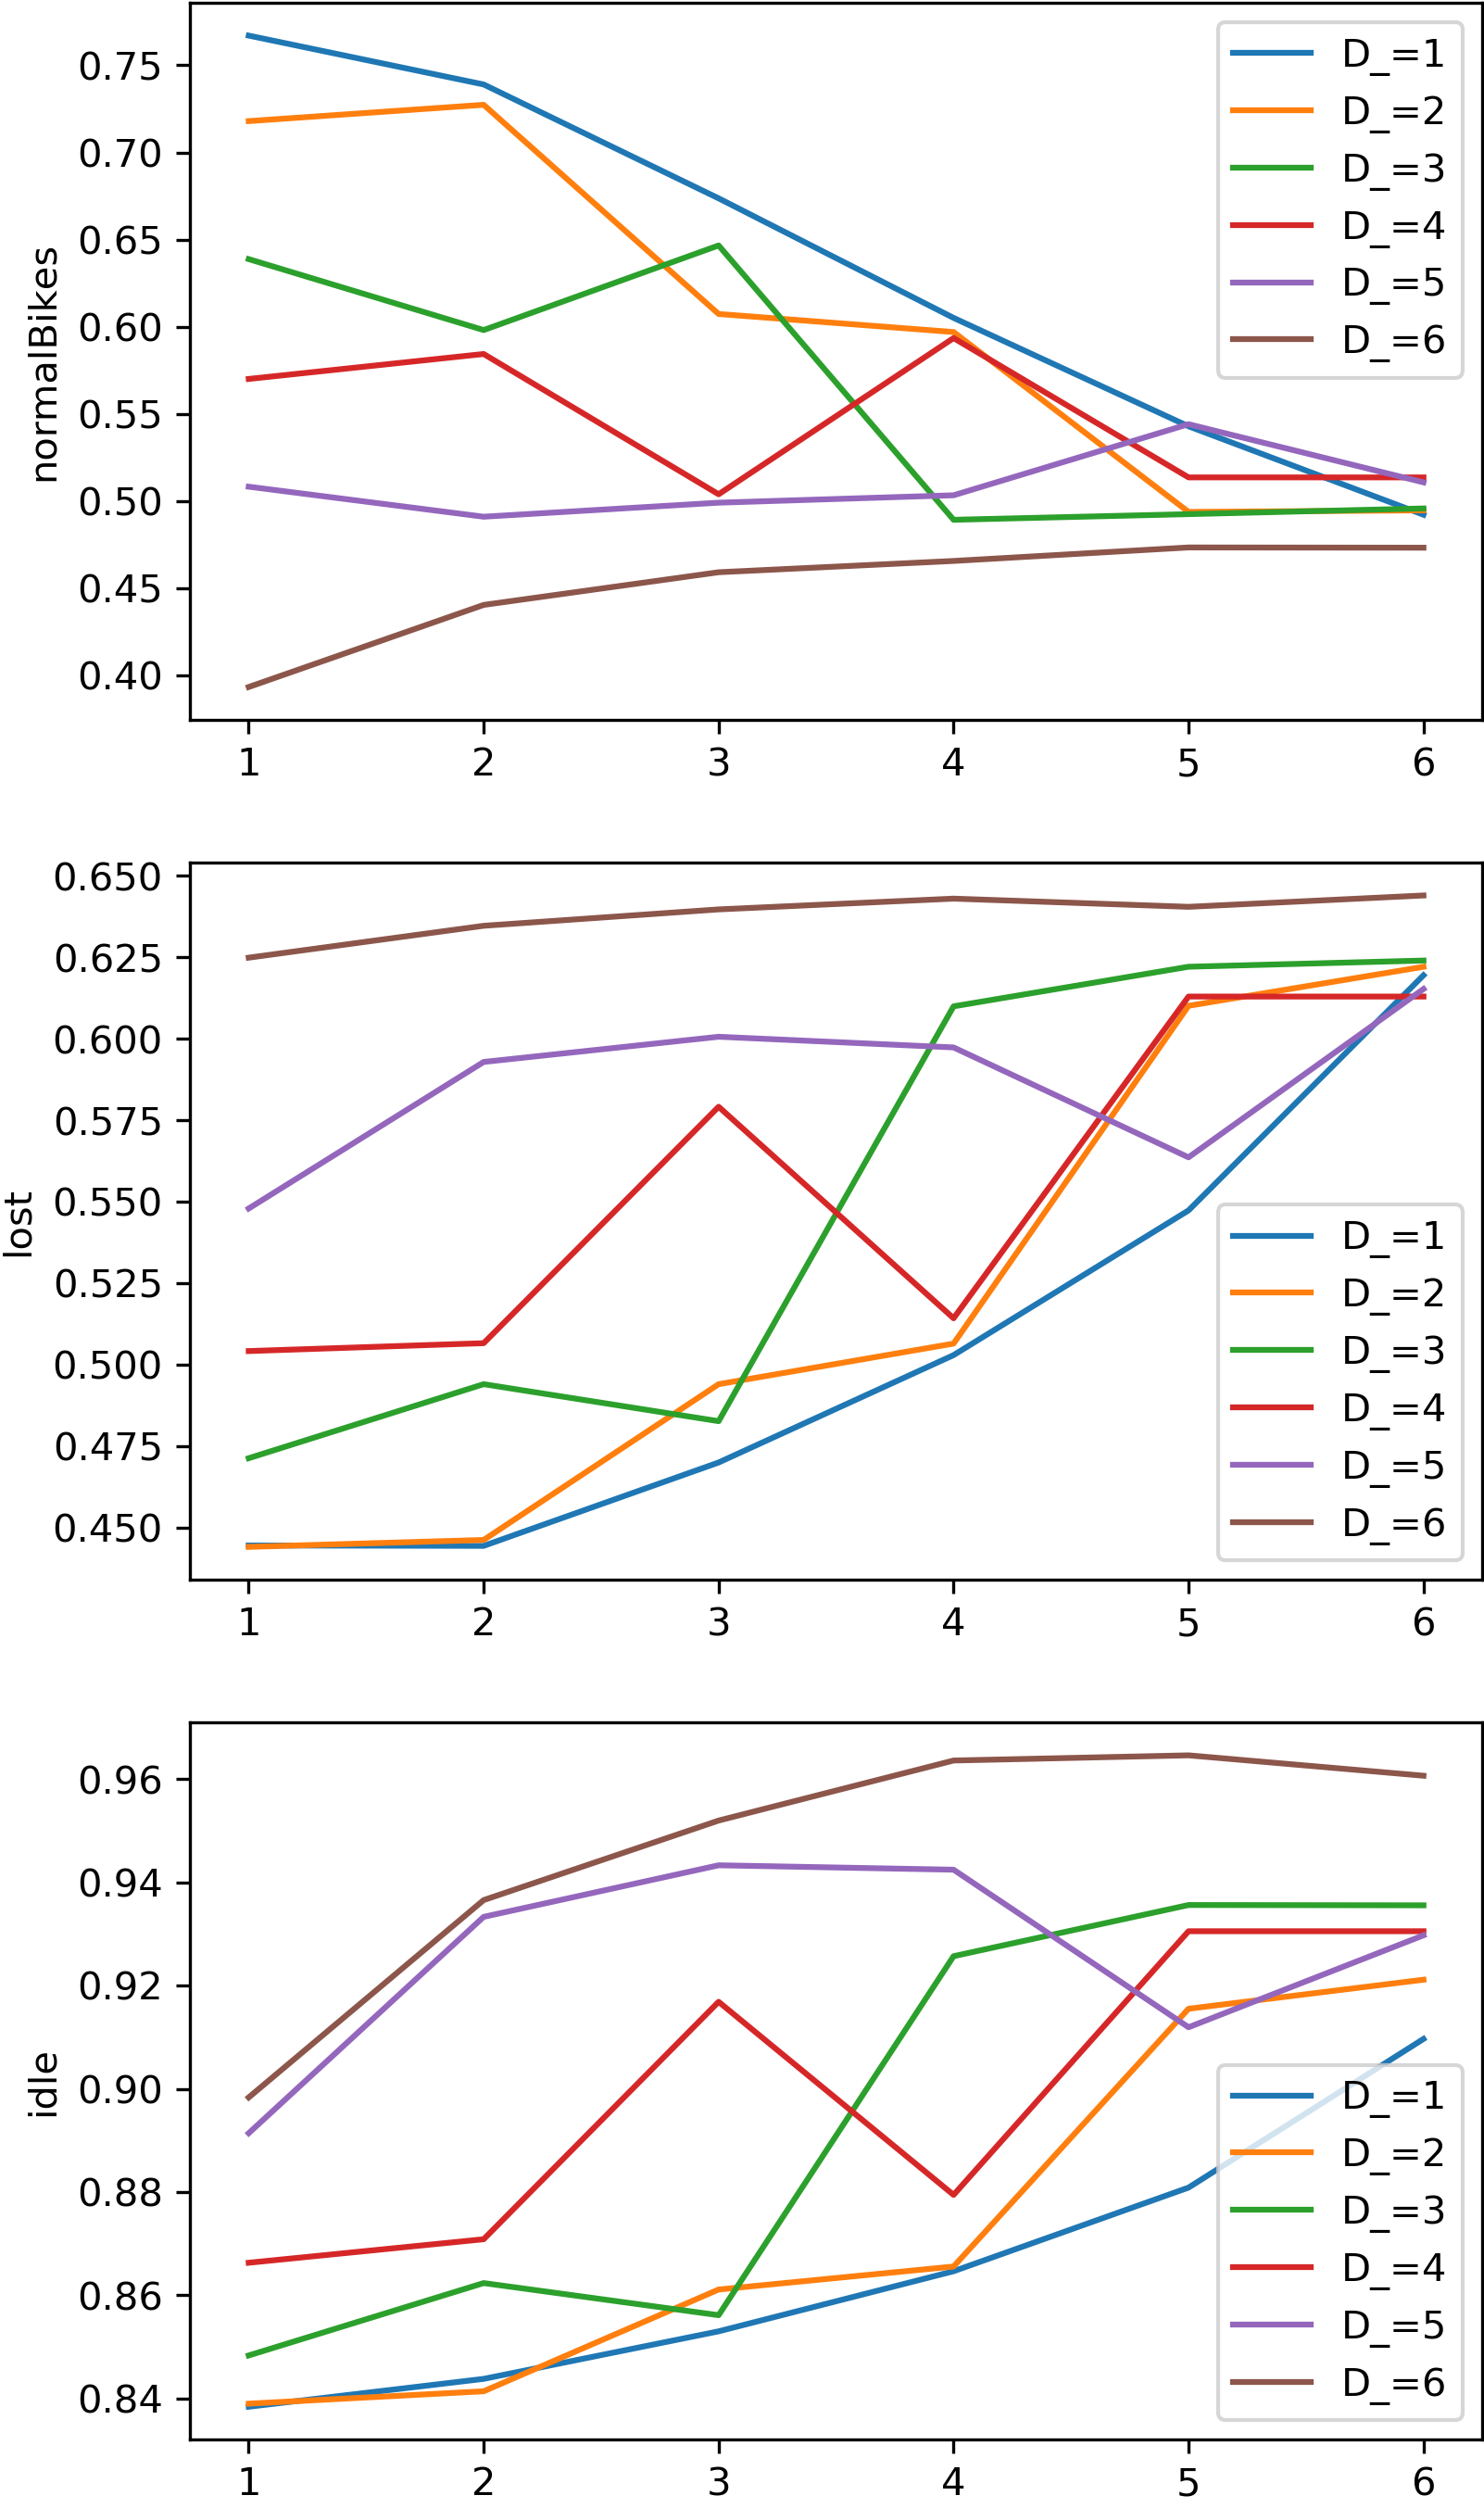
\includegraphics[width=2.3in]{Graph/perf/D_-B_.png}
%     %\caption{fig1}
%     \end{minipage}%
%     }%
%     % \caption{运维能力总量有限情况}
%     % \label{fig:fixsum}
% \end{figure}
%\restoregeometry



% \begin{itemize}
%     \item 损坏率升高,系统中的好车比例降低,顾客损失率普遍升高
%     \item 各个单个参数的效果
%     \item 每个部分的效果
%     \item 系统能力有限,在几个之间平衡时的效果
%     \item 维修速率的提高可以迅速改善系统的服务能力,但是单纯改善维修能力带来的改善是有限的,还会受到其他因素的限制。
%     \item 维修台带来的改善与维修速率类似,只是改善的程度更弱。
%     \item 损坏率的升高或者维修能力的改善,在某些情况下可能并不改善系统中顾客的损失情况
%     \item 对比而言,损坏率对两种模式有着显著不同的影响。在相同维修能力下,分散式的维修情况下系统中的好车数始终多于集中式维修。单独提升维修速度或者维修服务台的数量,维修的所能发挥的改善作用对二者而言是类似的,但是分散式的最大上限会更高。
%     \item 要匹配搬运能力、维修能力、维修台数量和投放能力,一个过高是没有意义的,边际效用递减
%     \item 搬运和投放能力相近时系统的好车比例最高
% \end{itemize}




% \newpage
% \normalsize\textbf{ 附录 }
% \begin{figure}[H]
%     \centering
%     \subfigure[时间长度]{
%     \begin{minipage}[t]{0.5\linewidth}
%     \centering
%     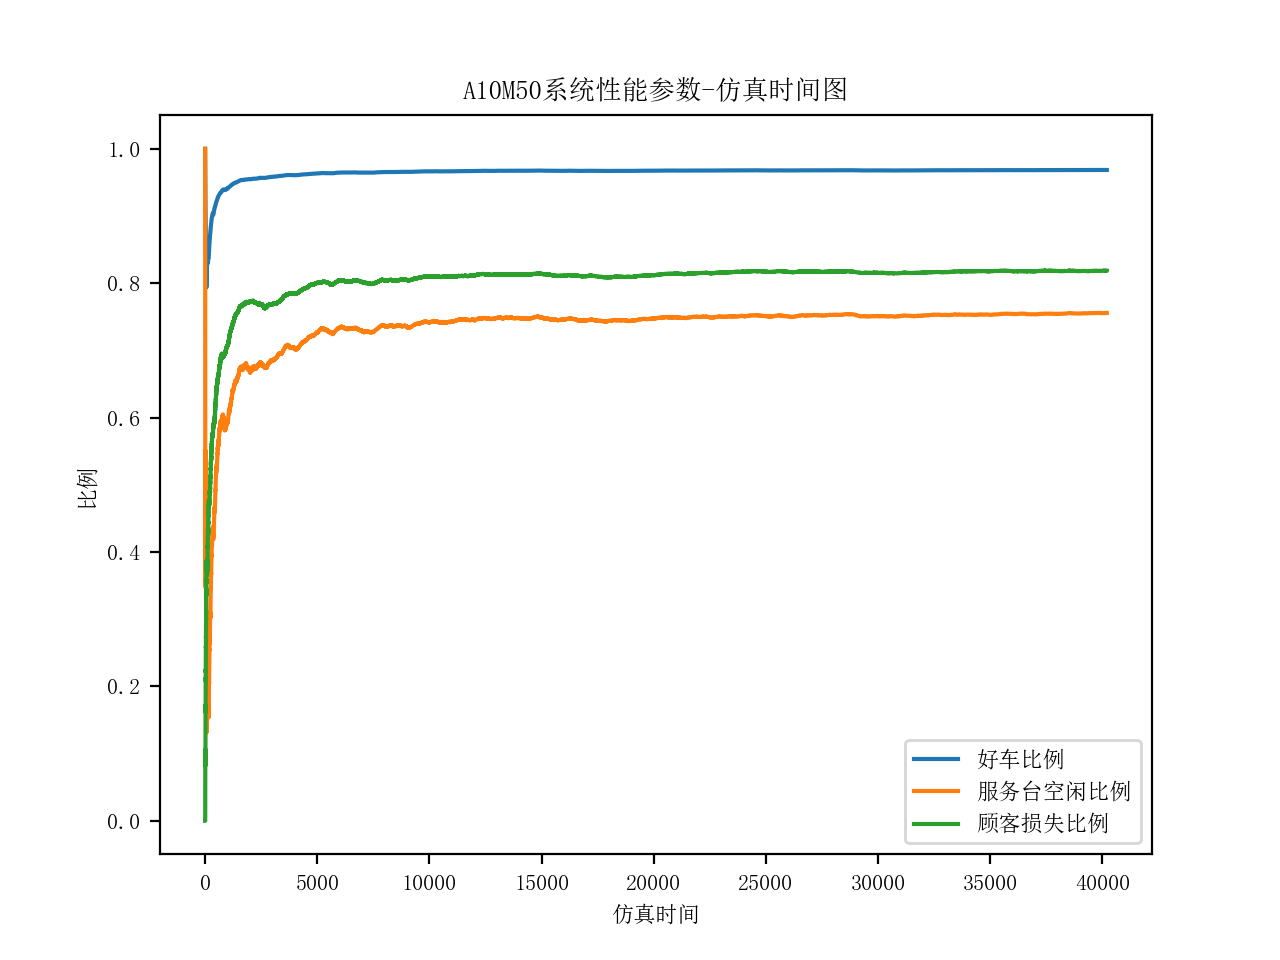
\includegraphics[width=2.4in]{Graph/A10M50系统性能参数-时间40000图.png}
%     %\caption{fig2}
%     \end{minipage}%
%     }%
% \end{figure}
% \begin{figure}[H]
%     \centering
%     \subfigure[$\overline{B}-\overline{D}$]{
%     \begin{minipage}[t]{0.5\linewidth}
%     \centering
%     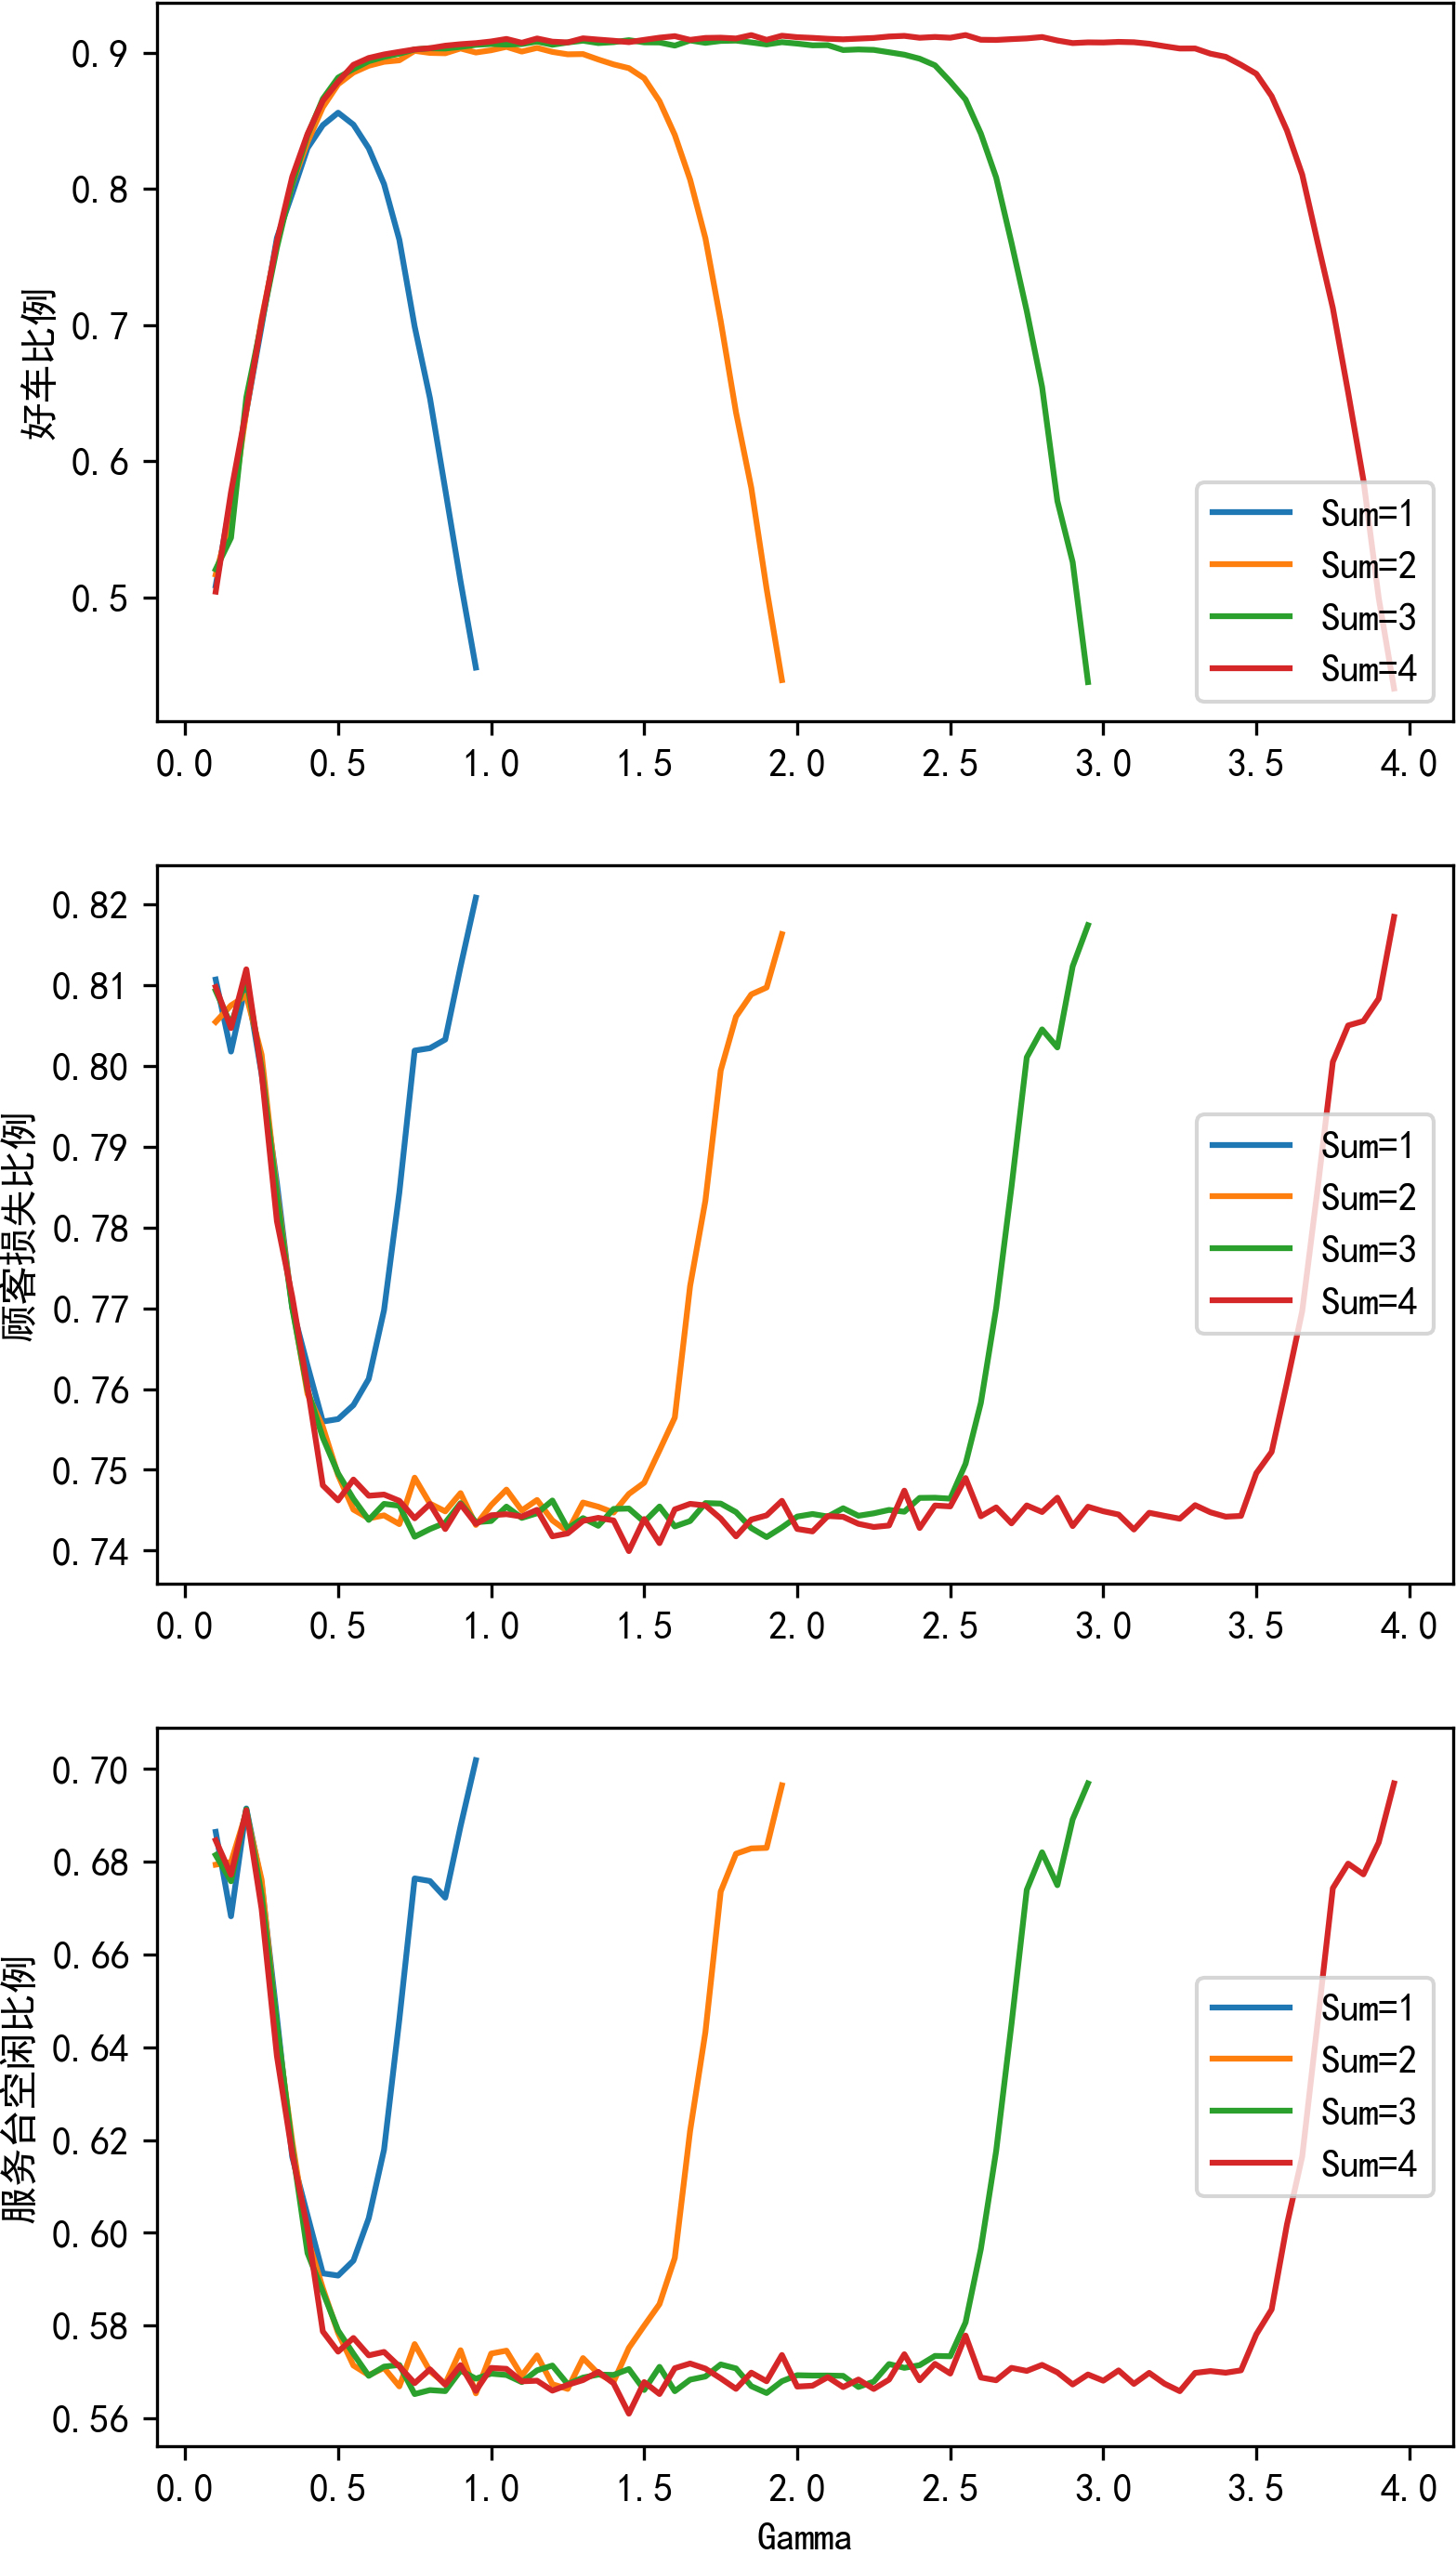
\includegraphics[width=2.3in]{Graph/perf/perfA10M50DeltaGammaSumVaryMu.png}
%     %\caption{fig1}
%     \end{minipage}%
%     }%
%     % \caption{运维能力总量有限情况}
%     % \label{fig:fixsum}
% \end{figure}

% \begin{figure}[H]
%     \centering
%     \subfigure[回收与投放速度总和为定值,变动总和]{
%     \begin{minipage}[t]{0.5\textwidth}
%     \centering
%     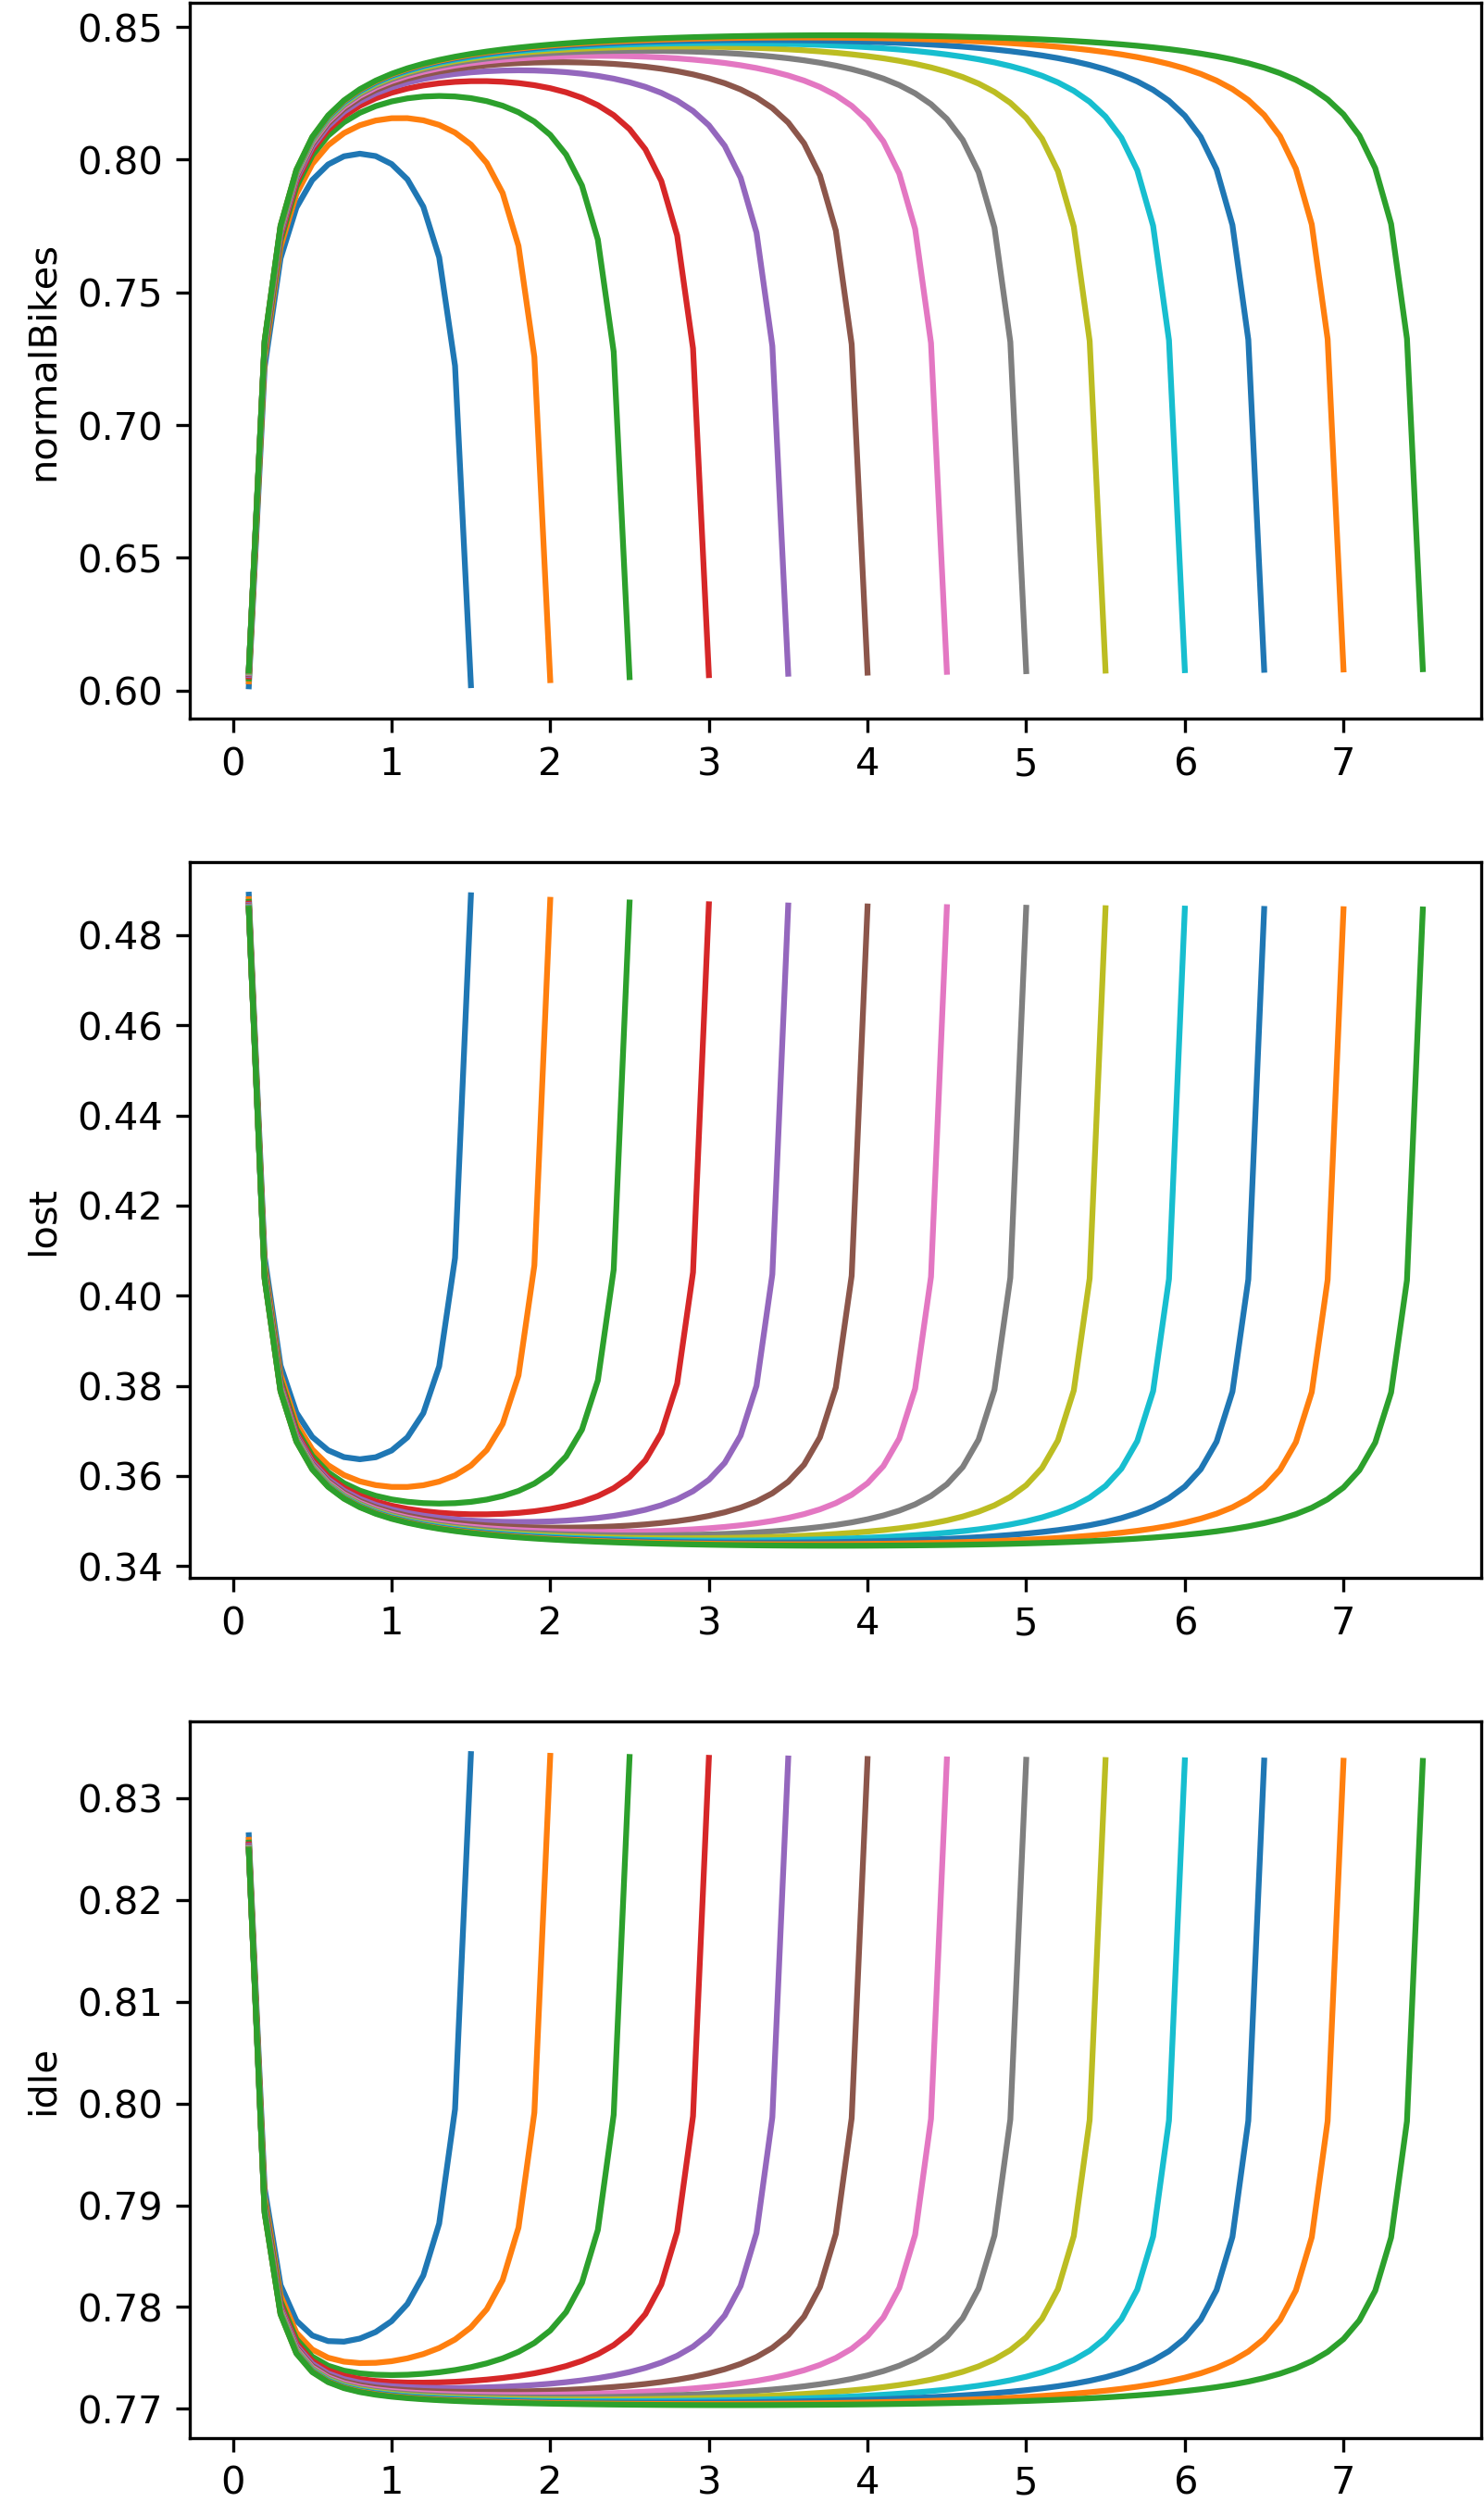
\includegraphics[width=2.4in]{Graph/perf/perfGamma+Delta0-Sum0-8lines.png}
%     %\caption{fig2}
%     \end{minipage}%
%     }%
%     \centering
%     \subfigure[回收与投放速度总和为定值,变动维修速率]{
%     \begin{minipage}[t]{0.5\textwidth}
%     \centering
%     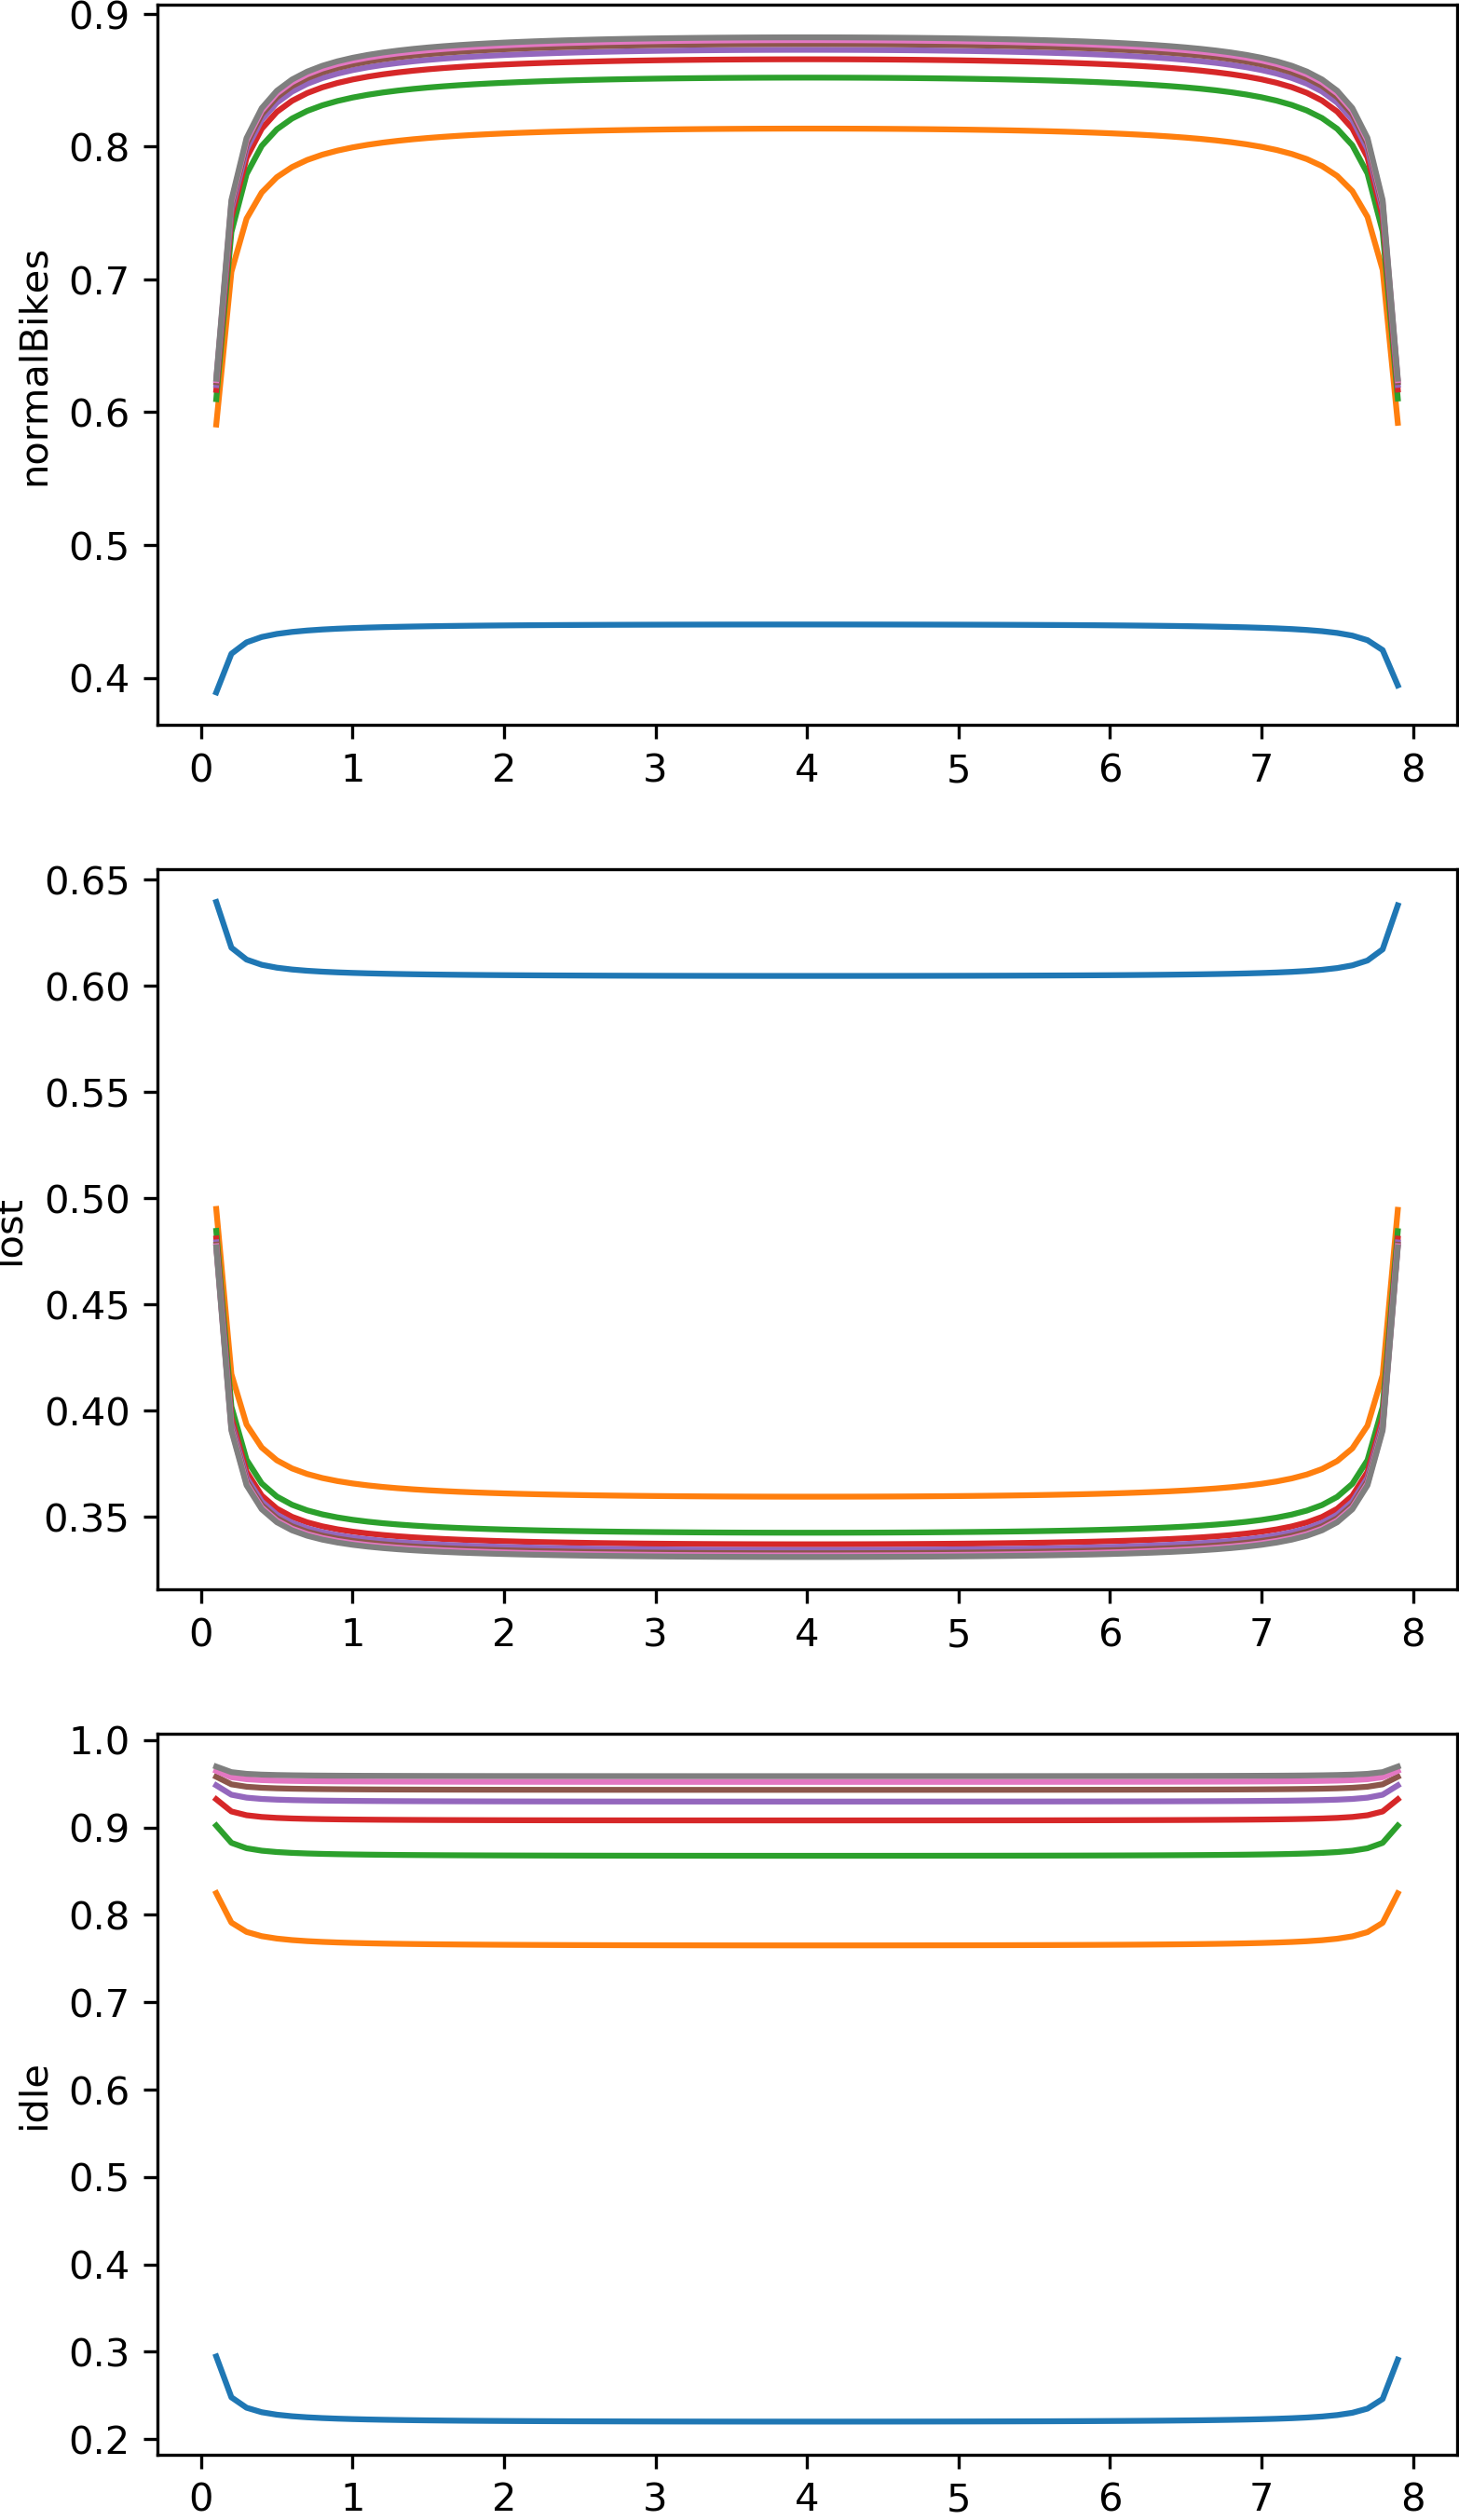
\includegraphics[width=2.3in]{Graph/perf/perfGamma+Delta0-8Mu0-4-8lines.png}
%     %\caption{fig1}
%     \end{minipage}%
%     }%xs
%     \label{fig:fixsum}
% \end{figure}

% \begin{figure}[H]
%     \centering
%     \subfigure[perfA10M50B\_-D\_1-7]{
%     \begin{minipage}[t]{0.5\textwidth}
%     \centering
%     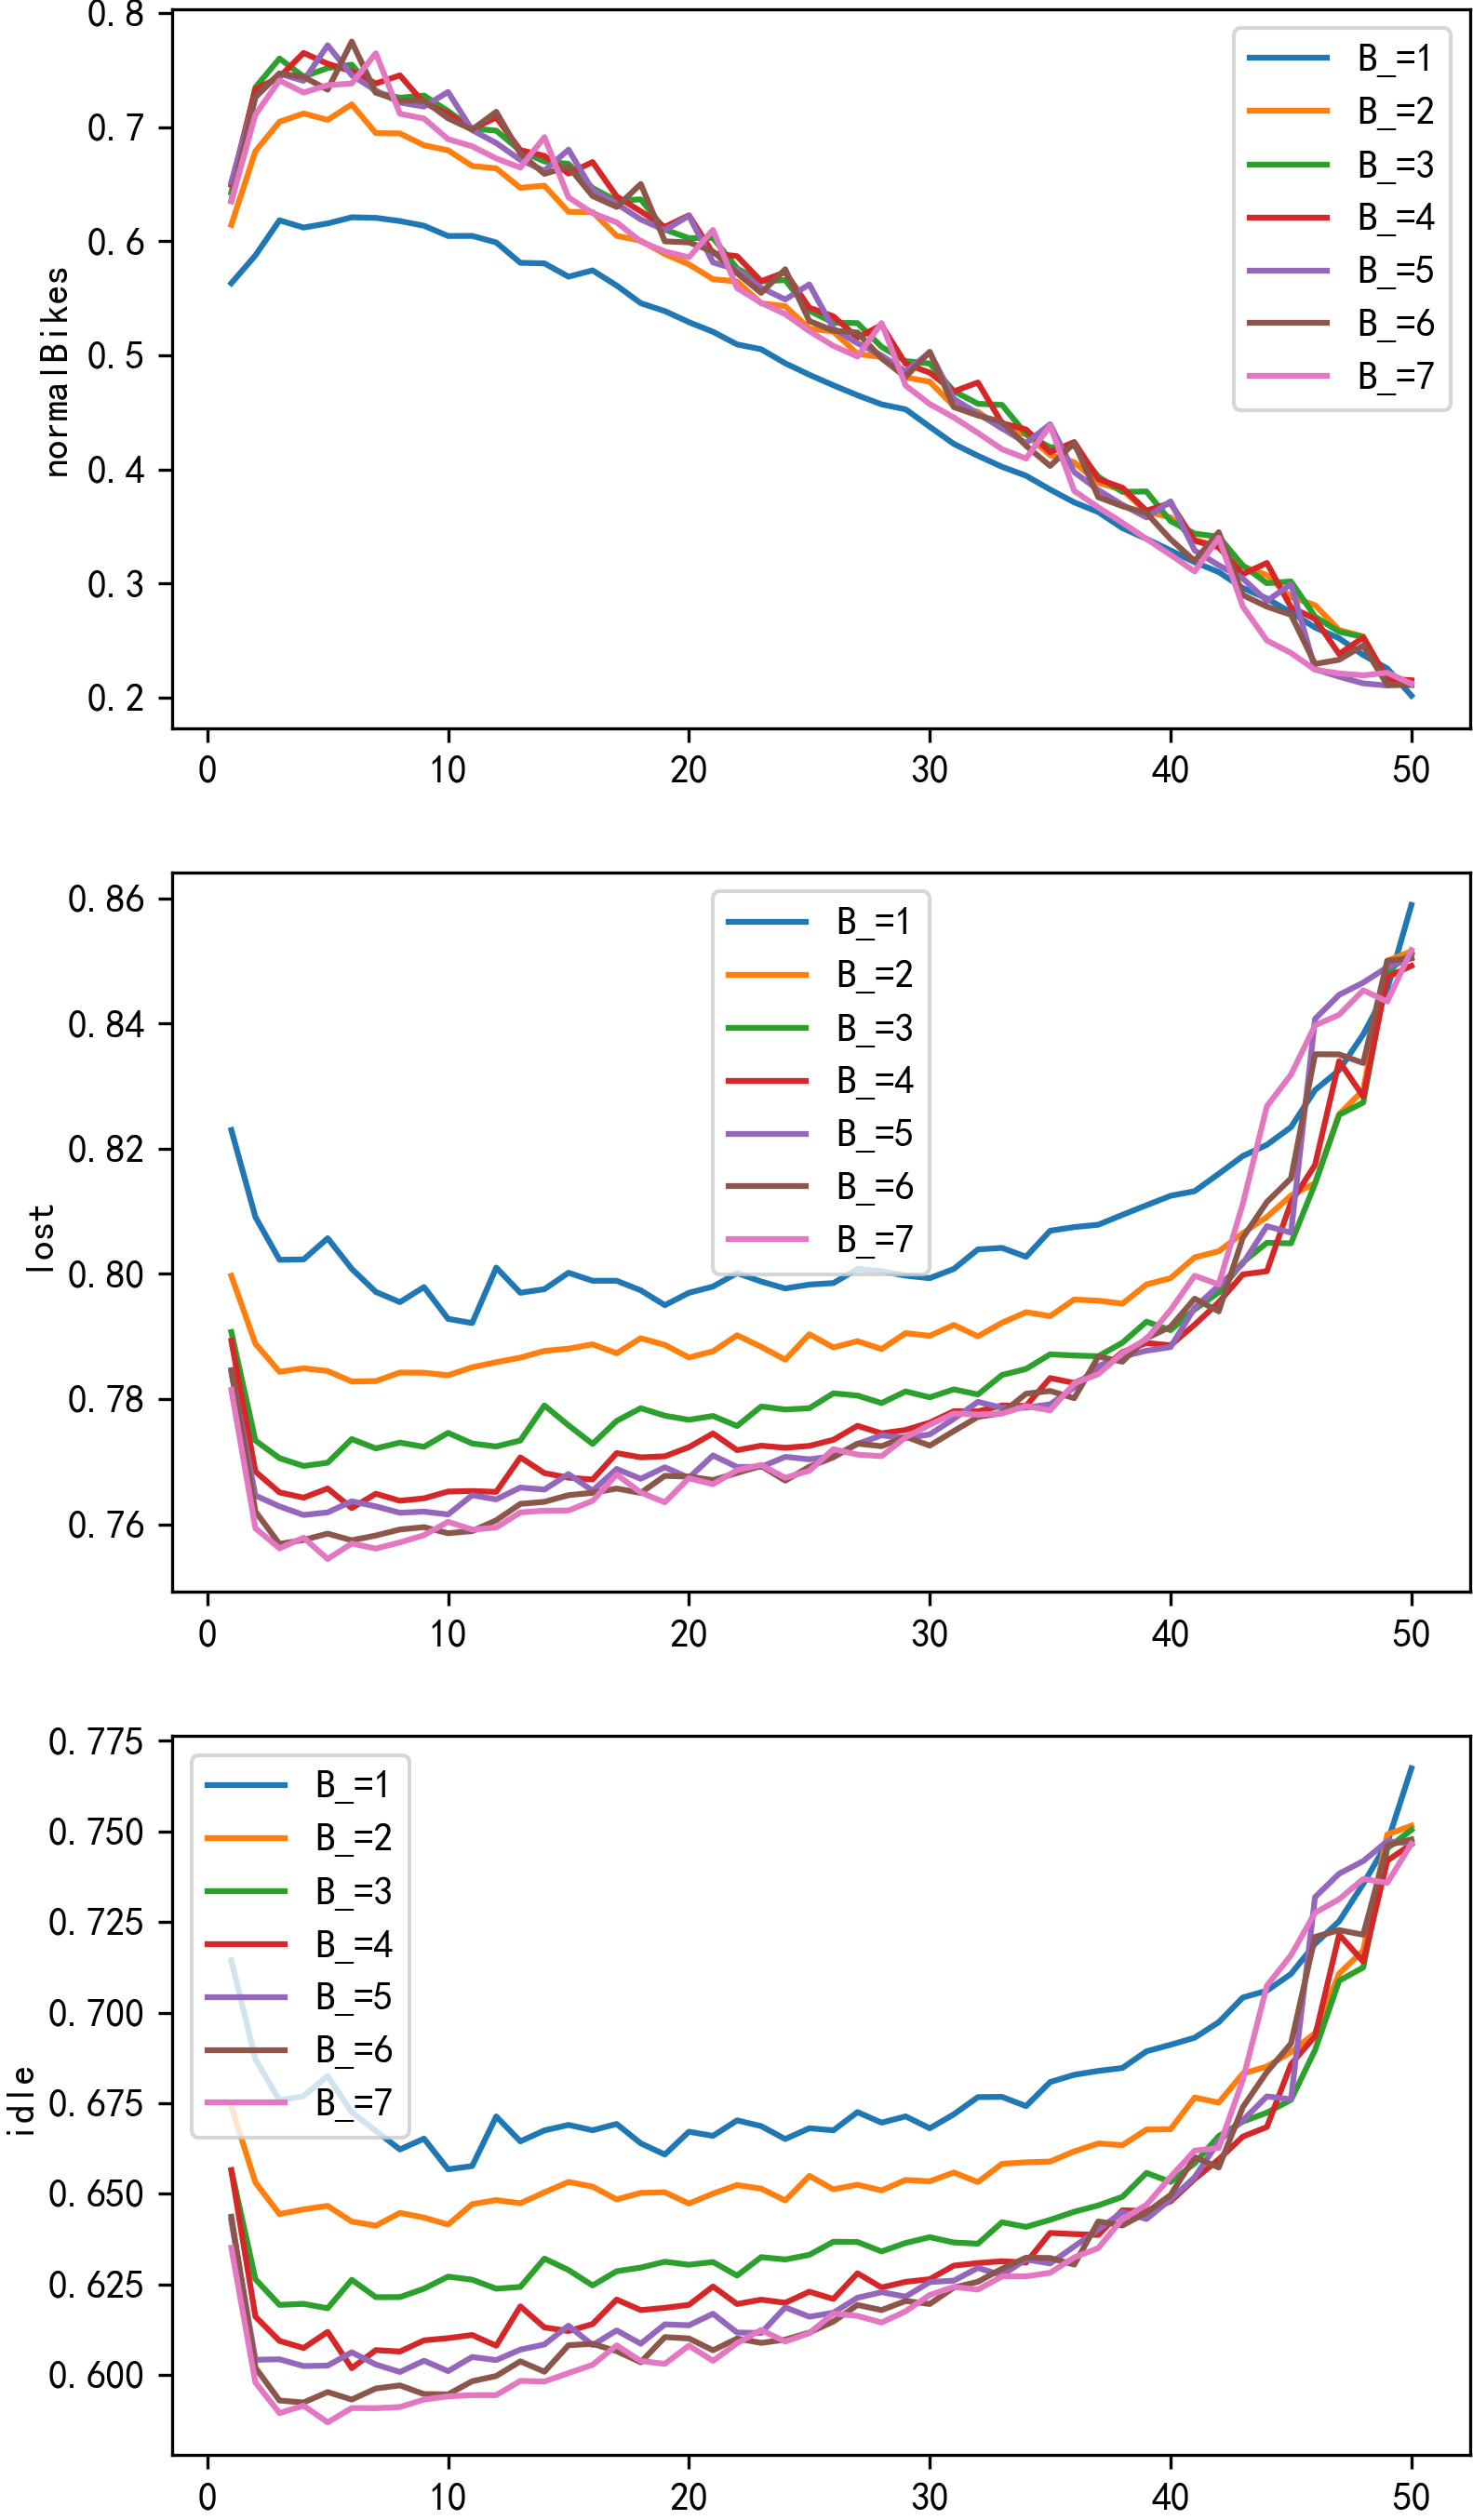
\includegraphics[width=2.3in]{Graph/perf/perfA10M50B_-D_1-7.png}
%     %\caption{fig1}
%     \end{minipage}%
%     }%xs
%     \centering
%     \subfigure[A10M50N1-50Mu0-4]{
%     \begin{minipage}[t]{0.5\textwidth}
%     \centering
%     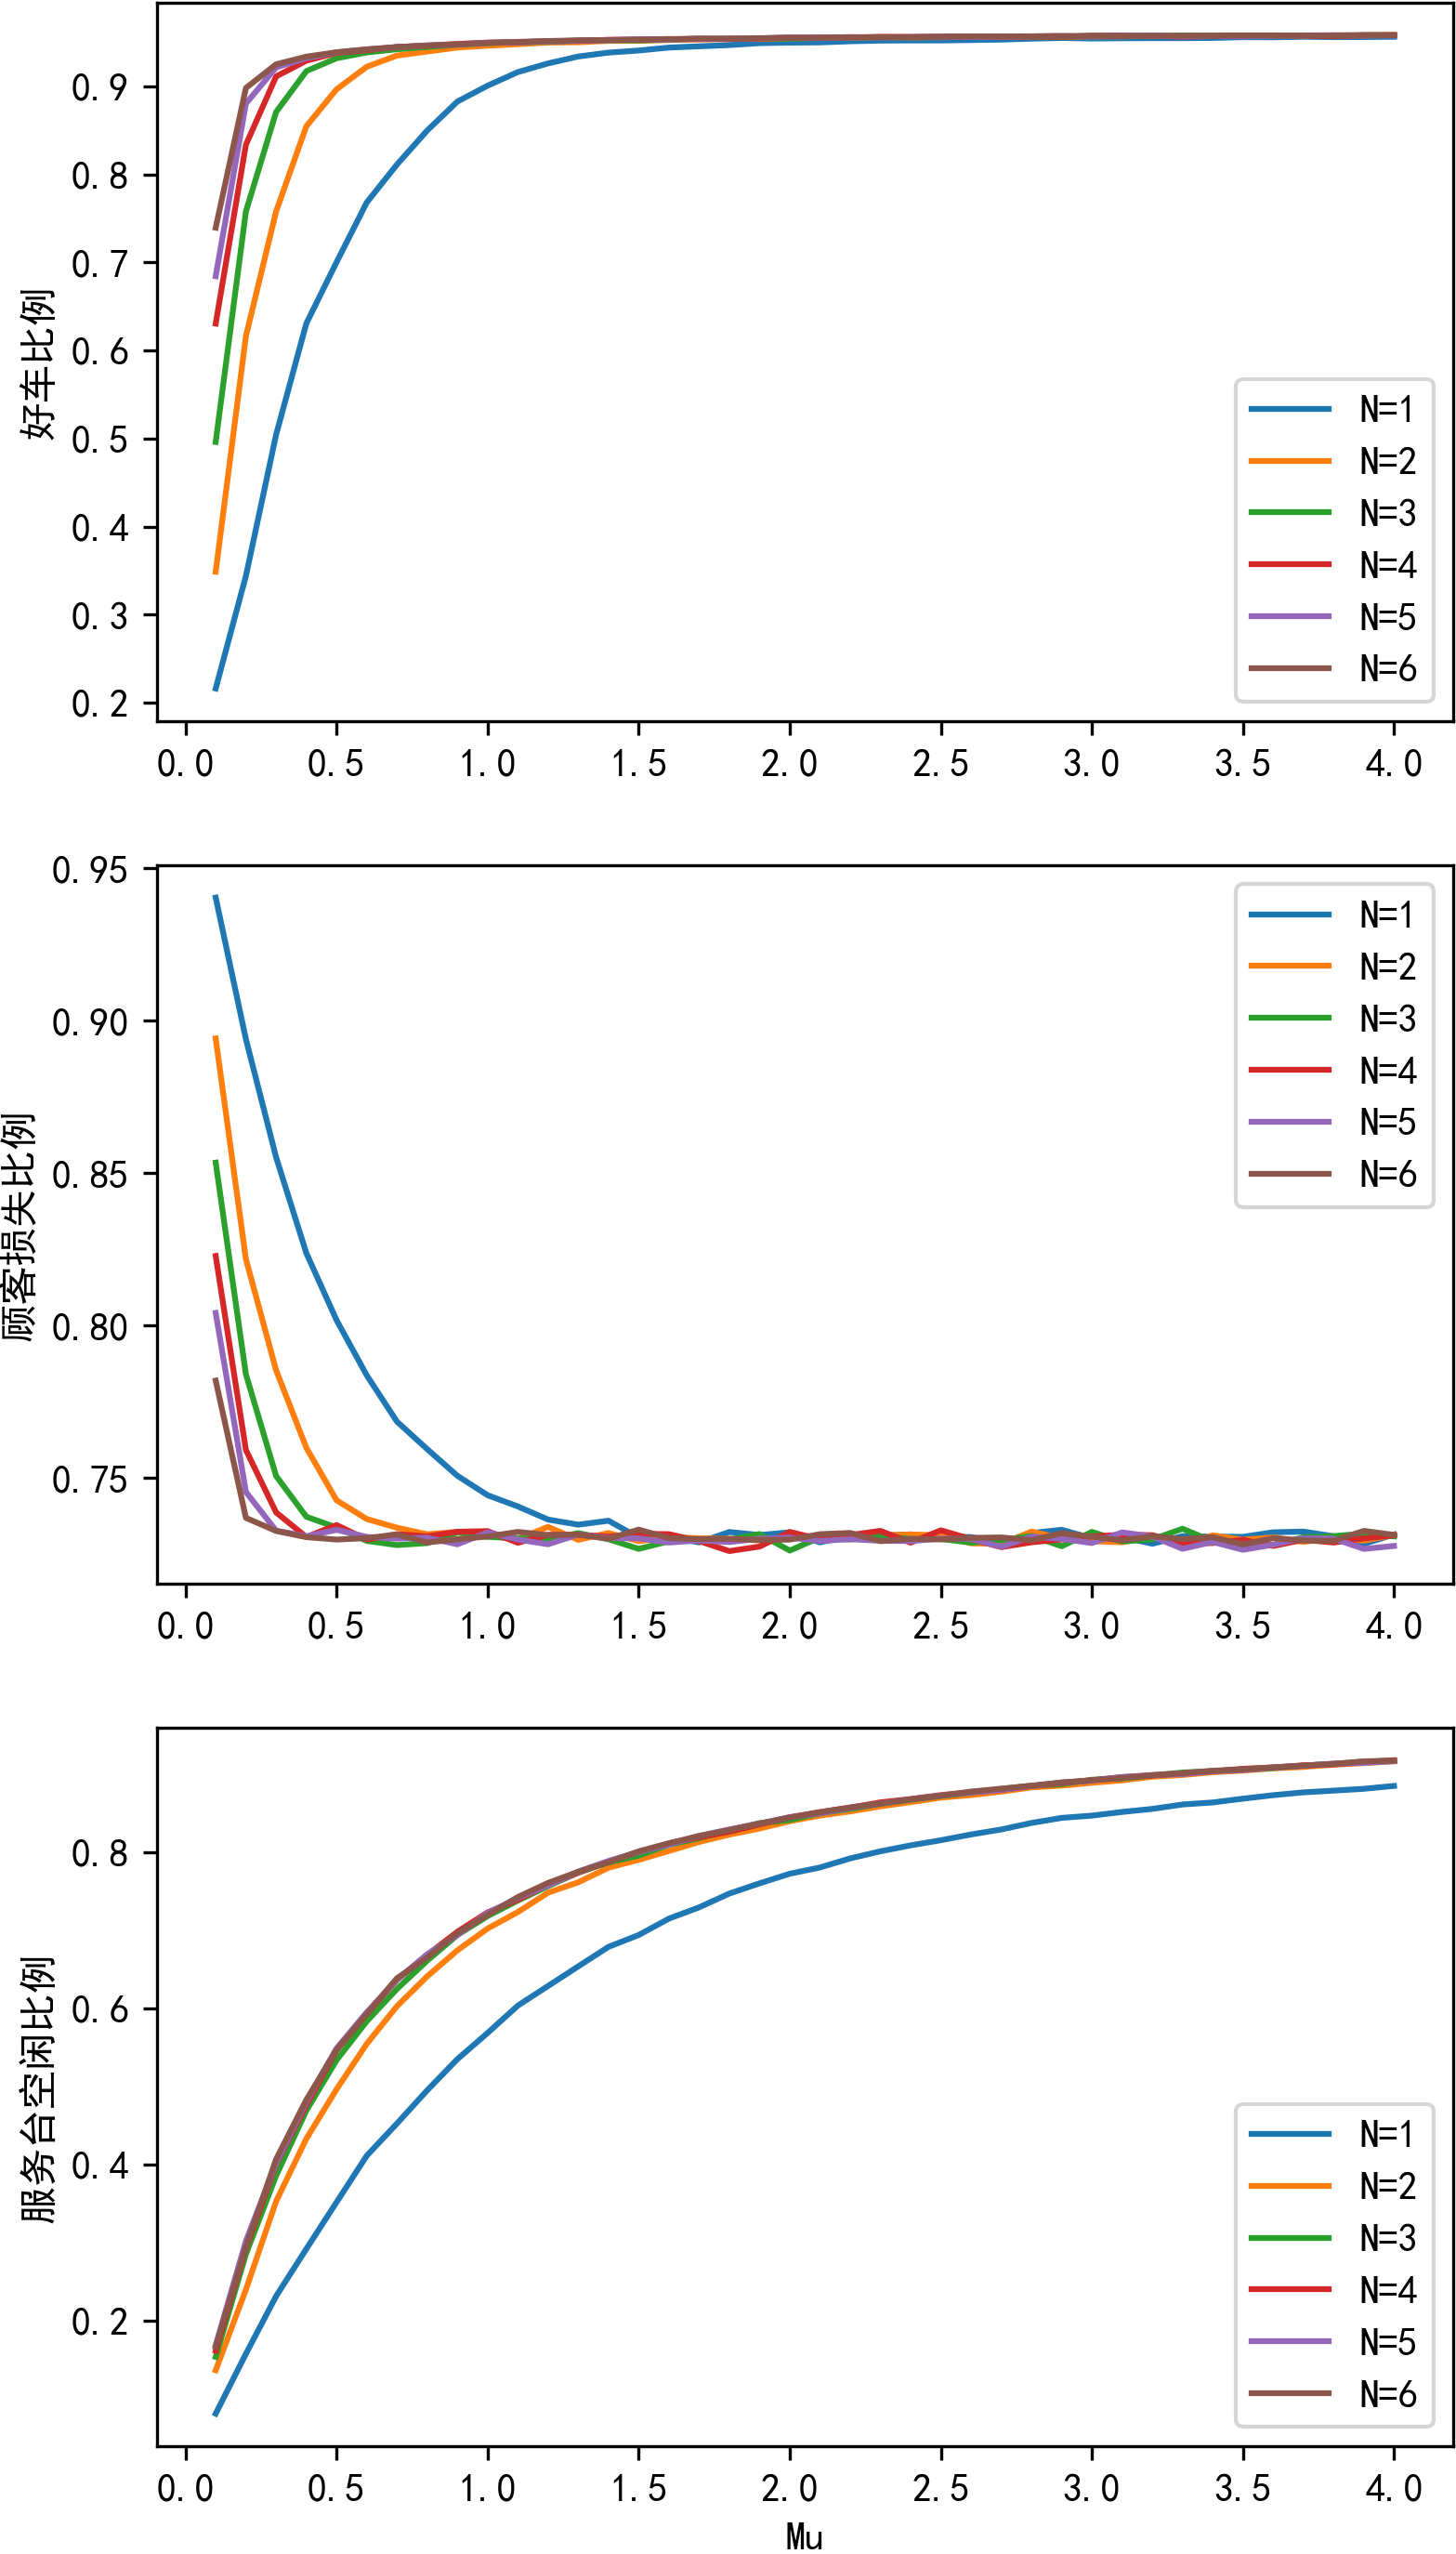
\includegraphics[width=2.3in]{Graph/perf/perfA10M50N1-50Mu0-4.png}
%     %\caption{fig1}
%     \end{minipage}%
%     }%xs
%     \caption{运维能力总量有限情况}
%     \label{fig:fixsum}
% \end{figure}

% \begin{figure}[H]
%     \centering
%     \subfigure[A10M50D\_1-50Delta0-4]{
%     \begin{minipage}[t]{0.5\textwidth}
%     \centering
%     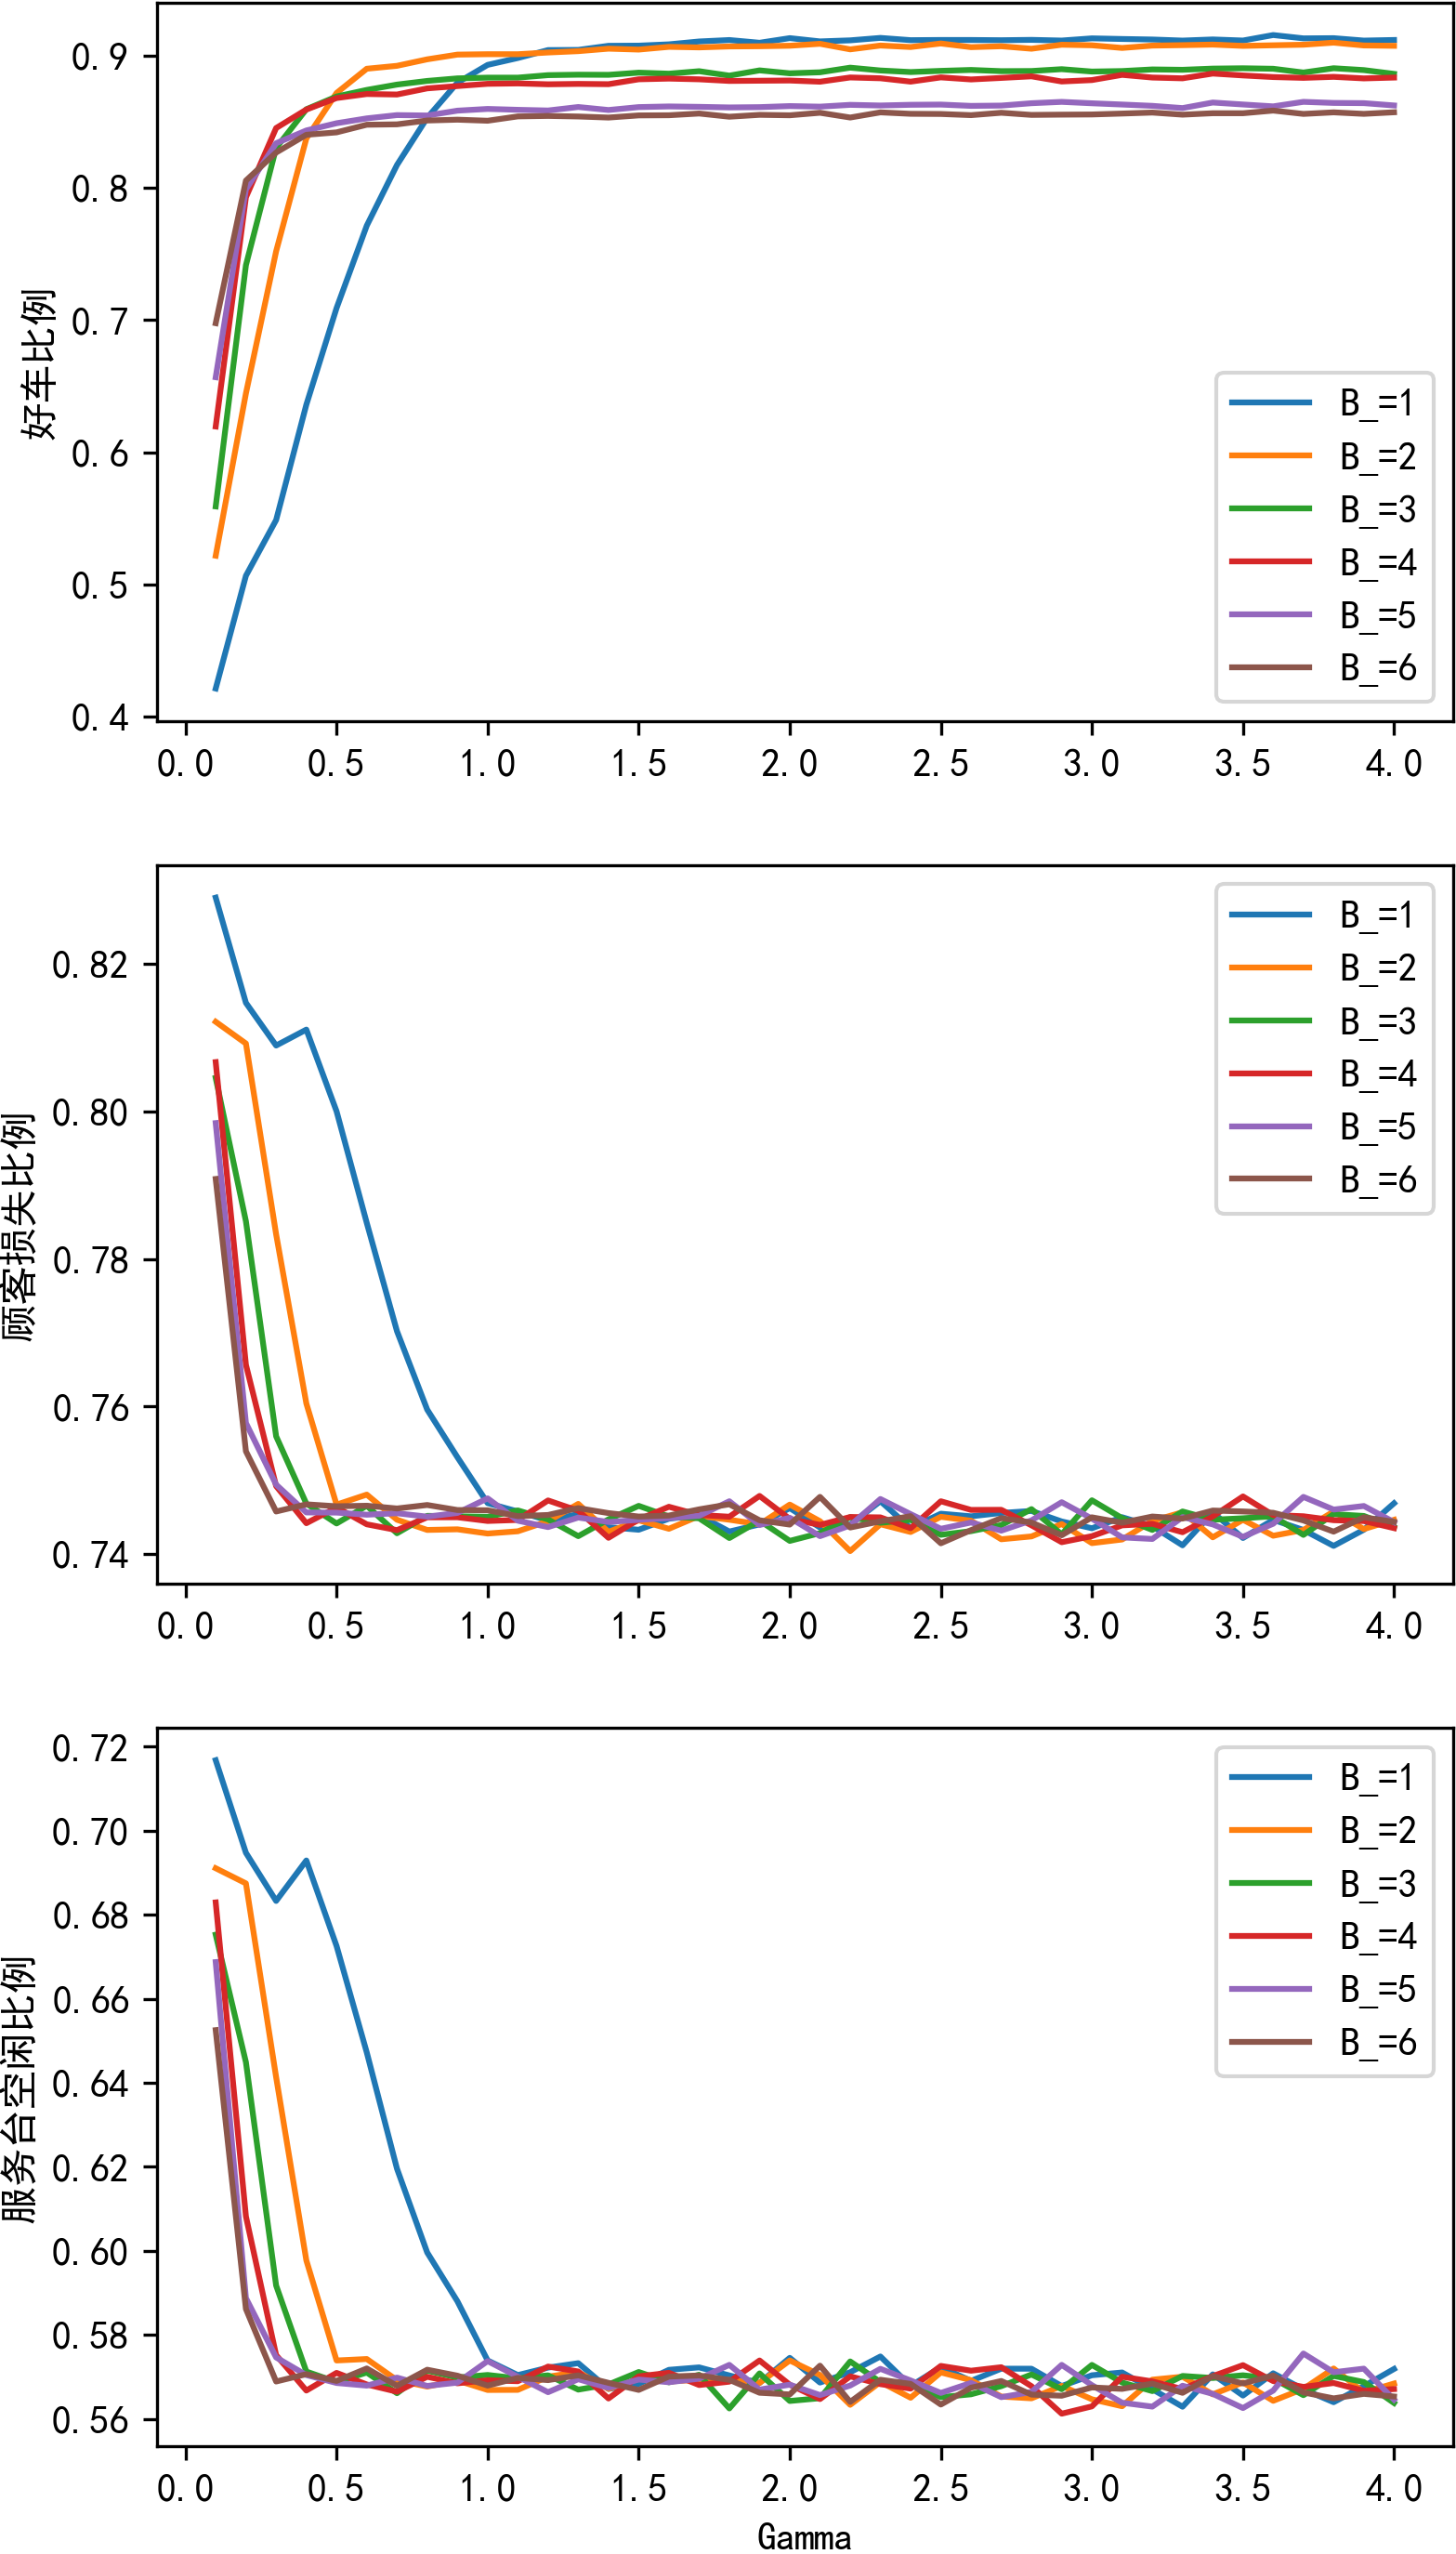
\includegraphics[width=2.3in]{Graph/perf/perfA10M50D_1-50Delta0-4.png}
%     %\caption{fig1}
%     \end{minipage}%
%     }%xs
%     \centering
%     \subfigure[A10M50B\_1-6Gamma0-4]{
%     \begin{minipage}[t]{0.5\textwidth}
%     \centering
%     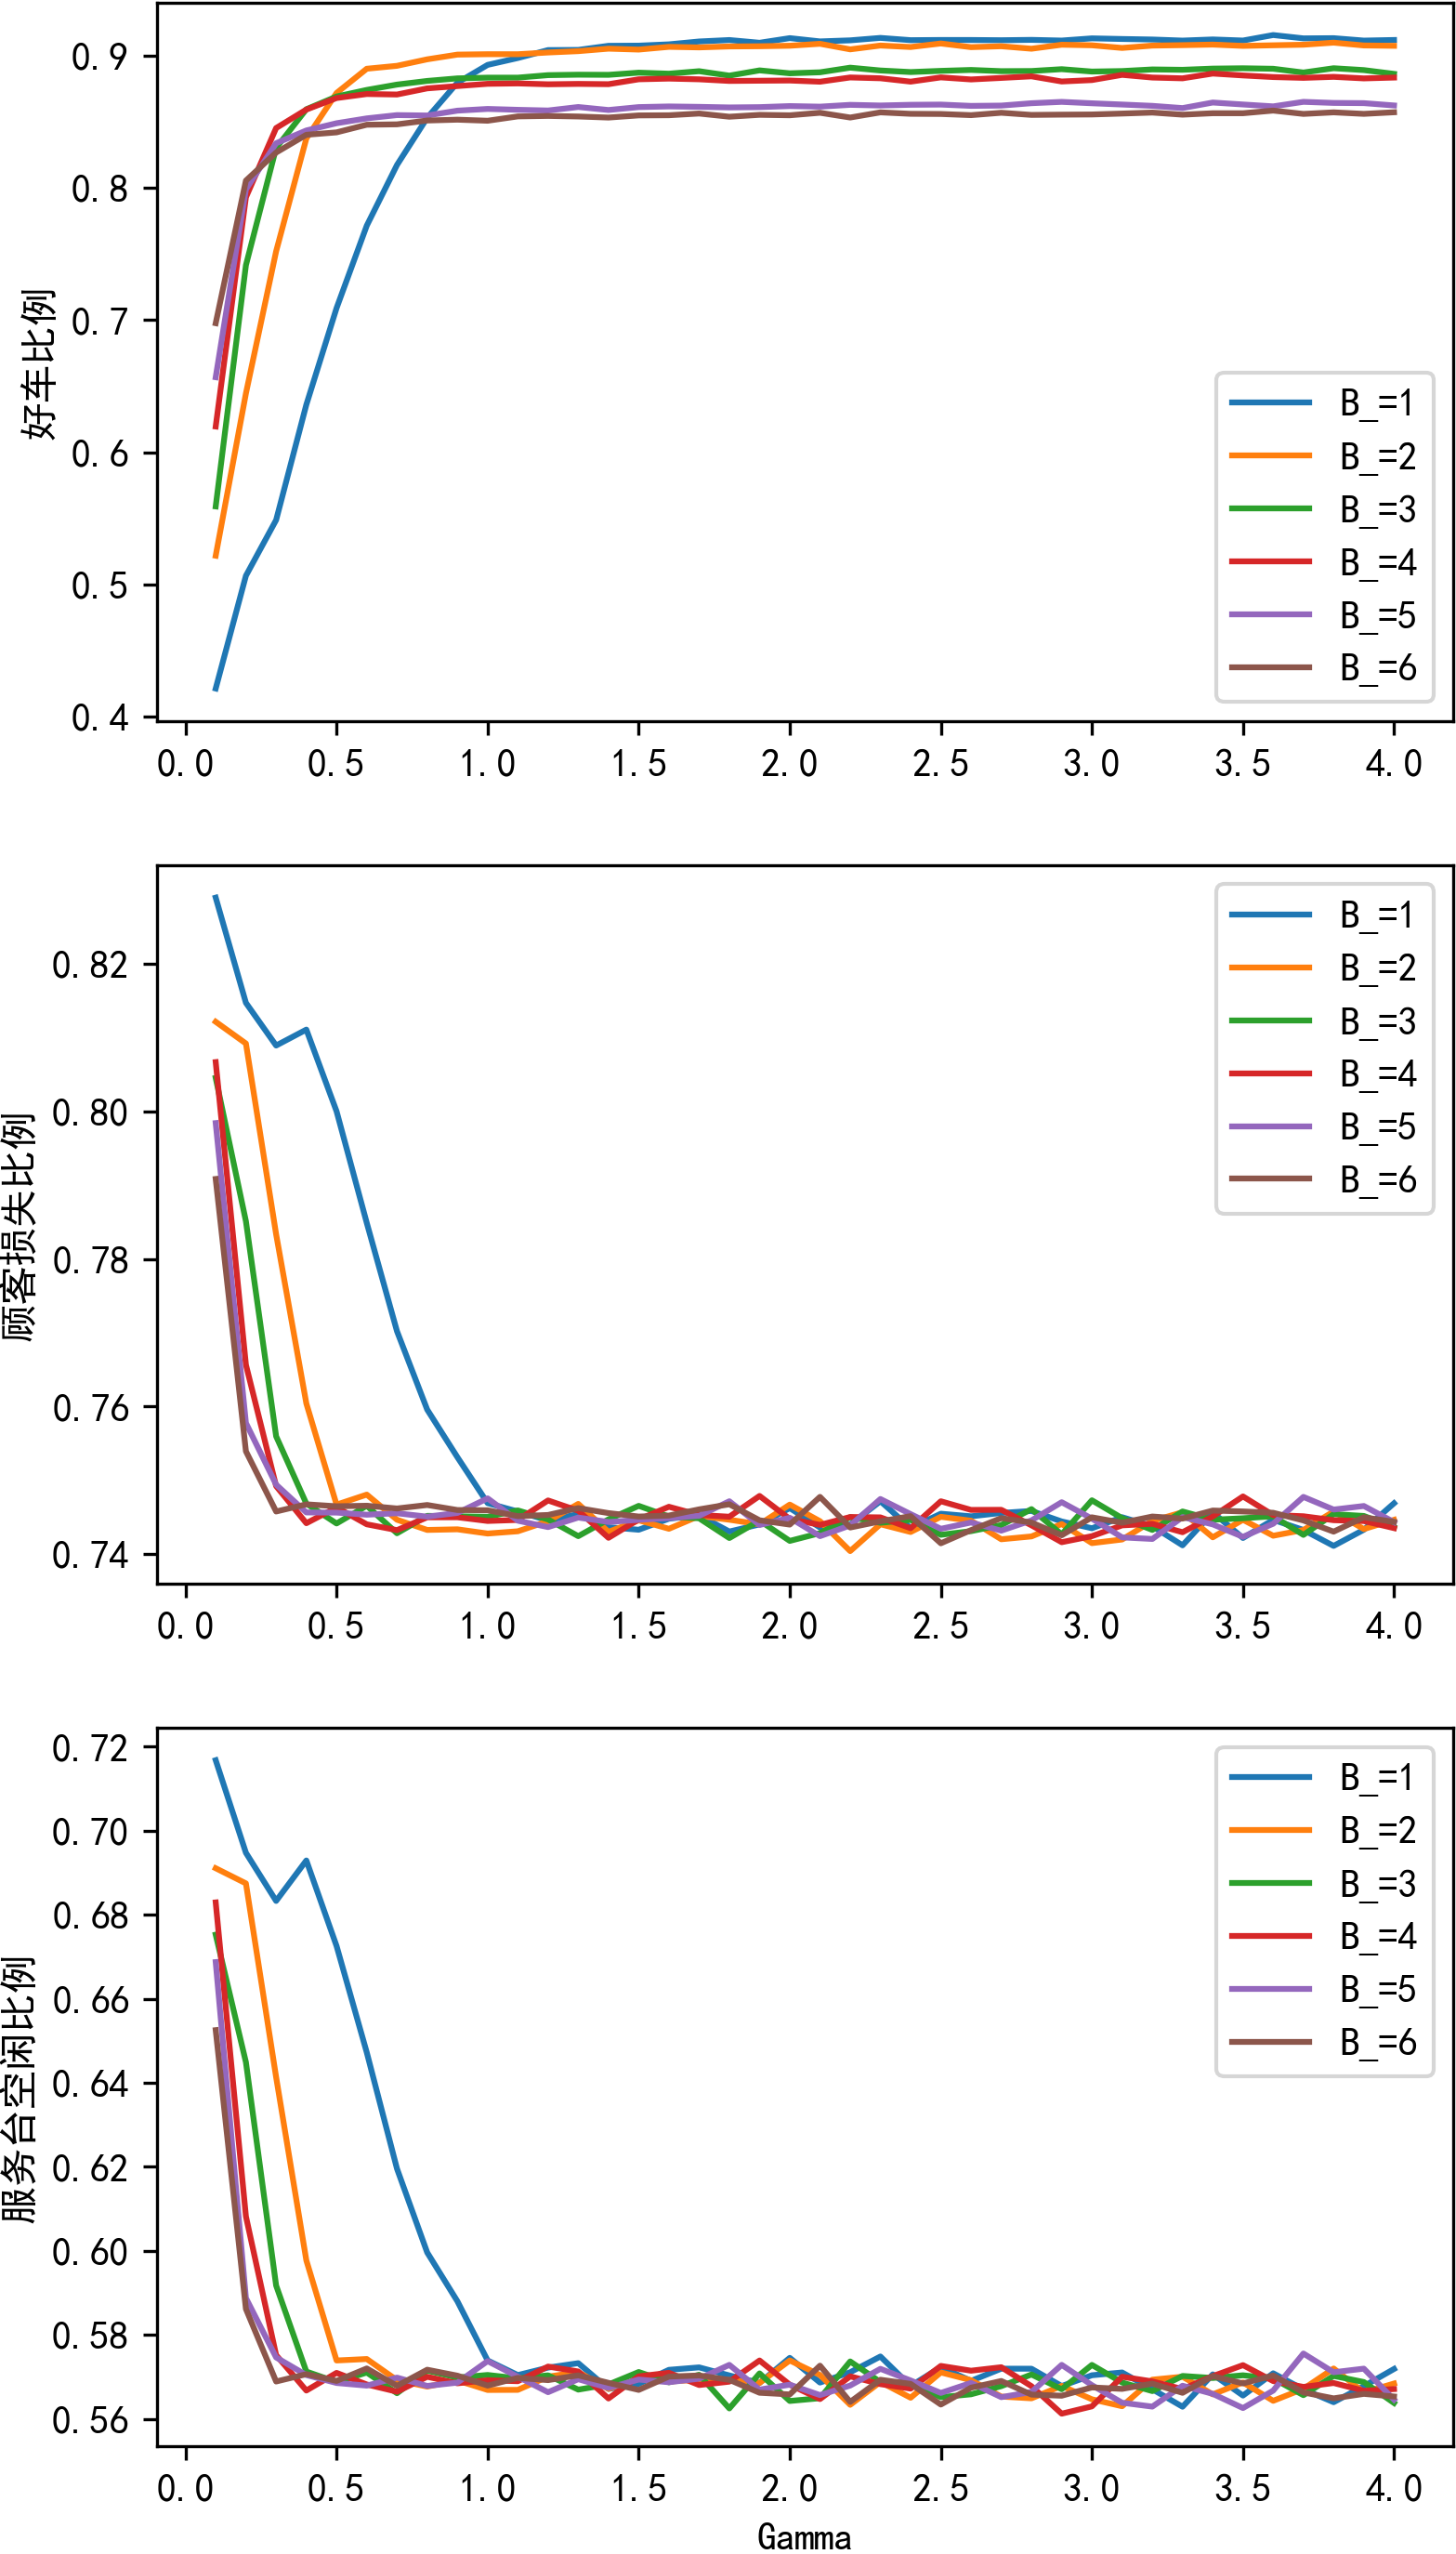
\includegraphics[width=2.3in]{Graph/perf/perfA10M50B_1-6Gamma0-4.png}
%     %\caption{fig1}
%     \end{minipage}%
%     }%xs
%     \caption{运维能力总量有限情况}
%     \label{fig:fixsum}
% \end{figure}



% \newgeometry{left=0.1cm,right=0.1cm, top=0.1cm, bottom=0.1cm}
% \begin{figure}[h]
%     \centering
%     \subfigure[Gamma]{
%     \begin{minipage}[t]{0.5\linewidth}
%     \centering
%     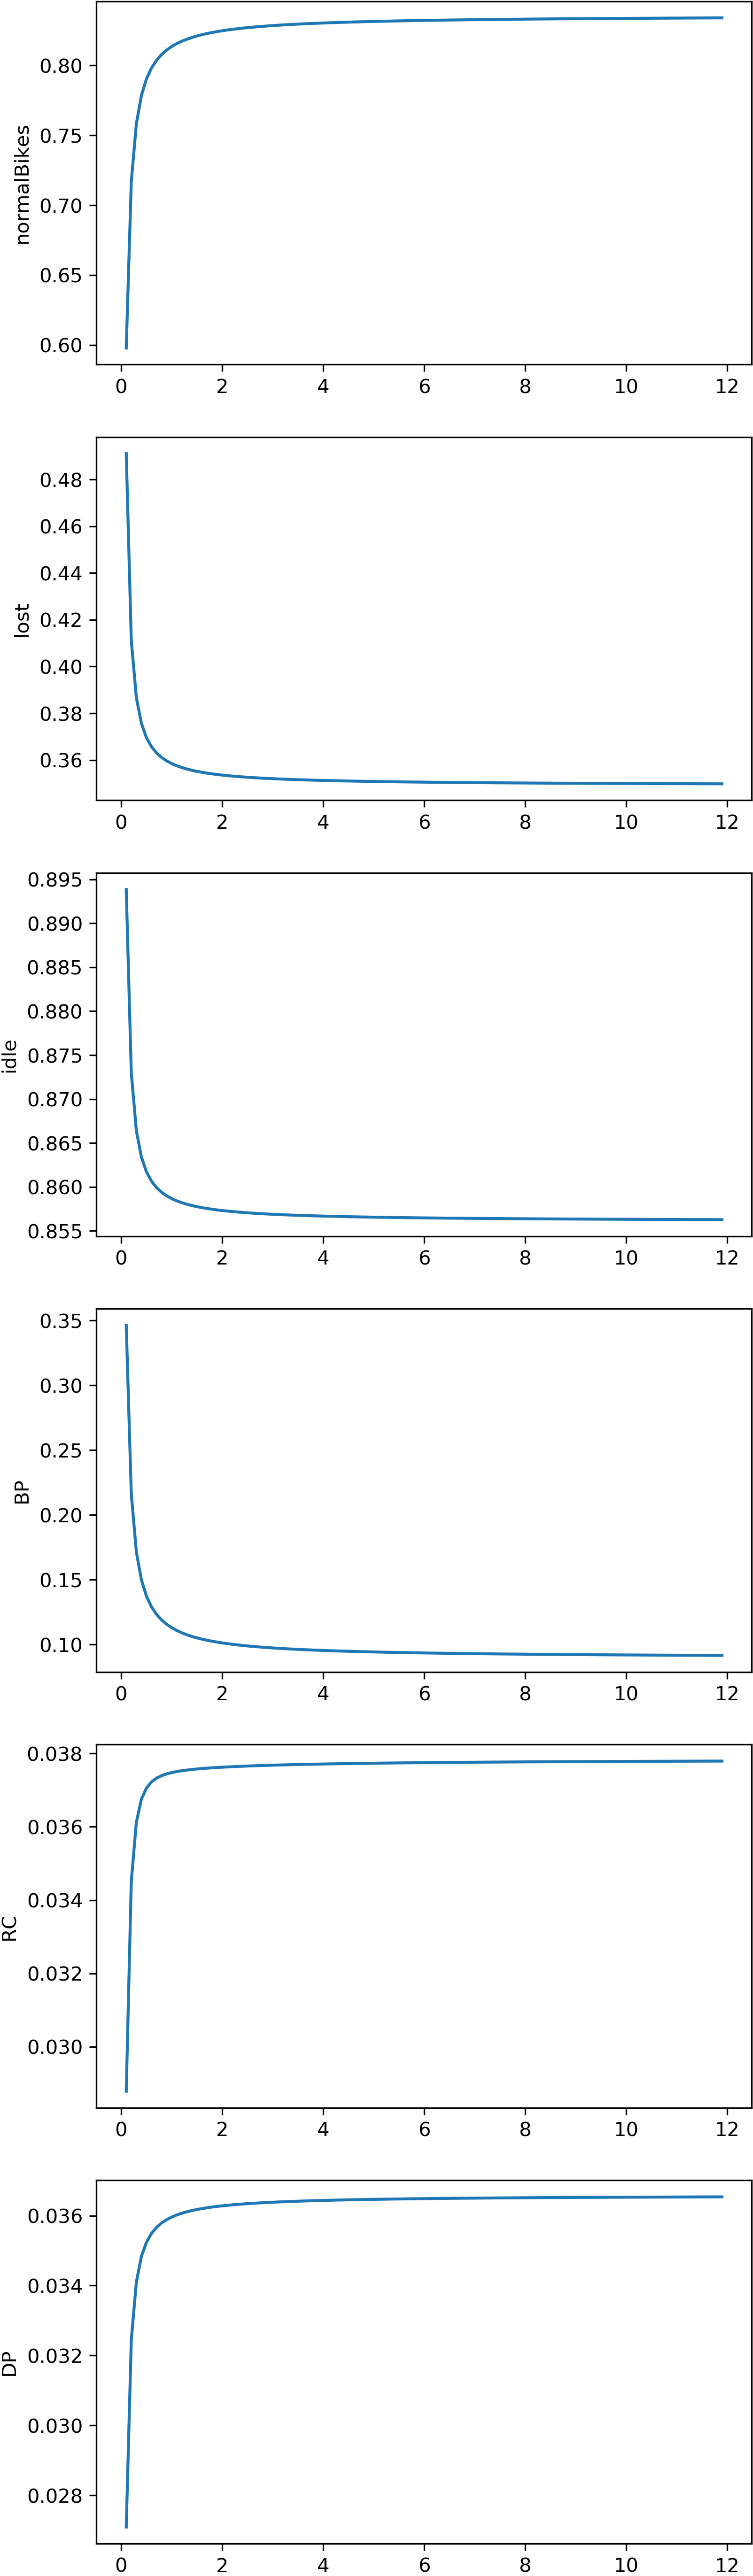
\includegraphics[width=2.3in]{Graph/perfGamma0-12.png}
%     %\caption{fig1}
%     \end{minipage}%
%     }%
%     \centering
%     \subfigure[$\overline{B}$]{
%     \begin{minipage}[t]{0.5\linewidth}
%     \centering
%     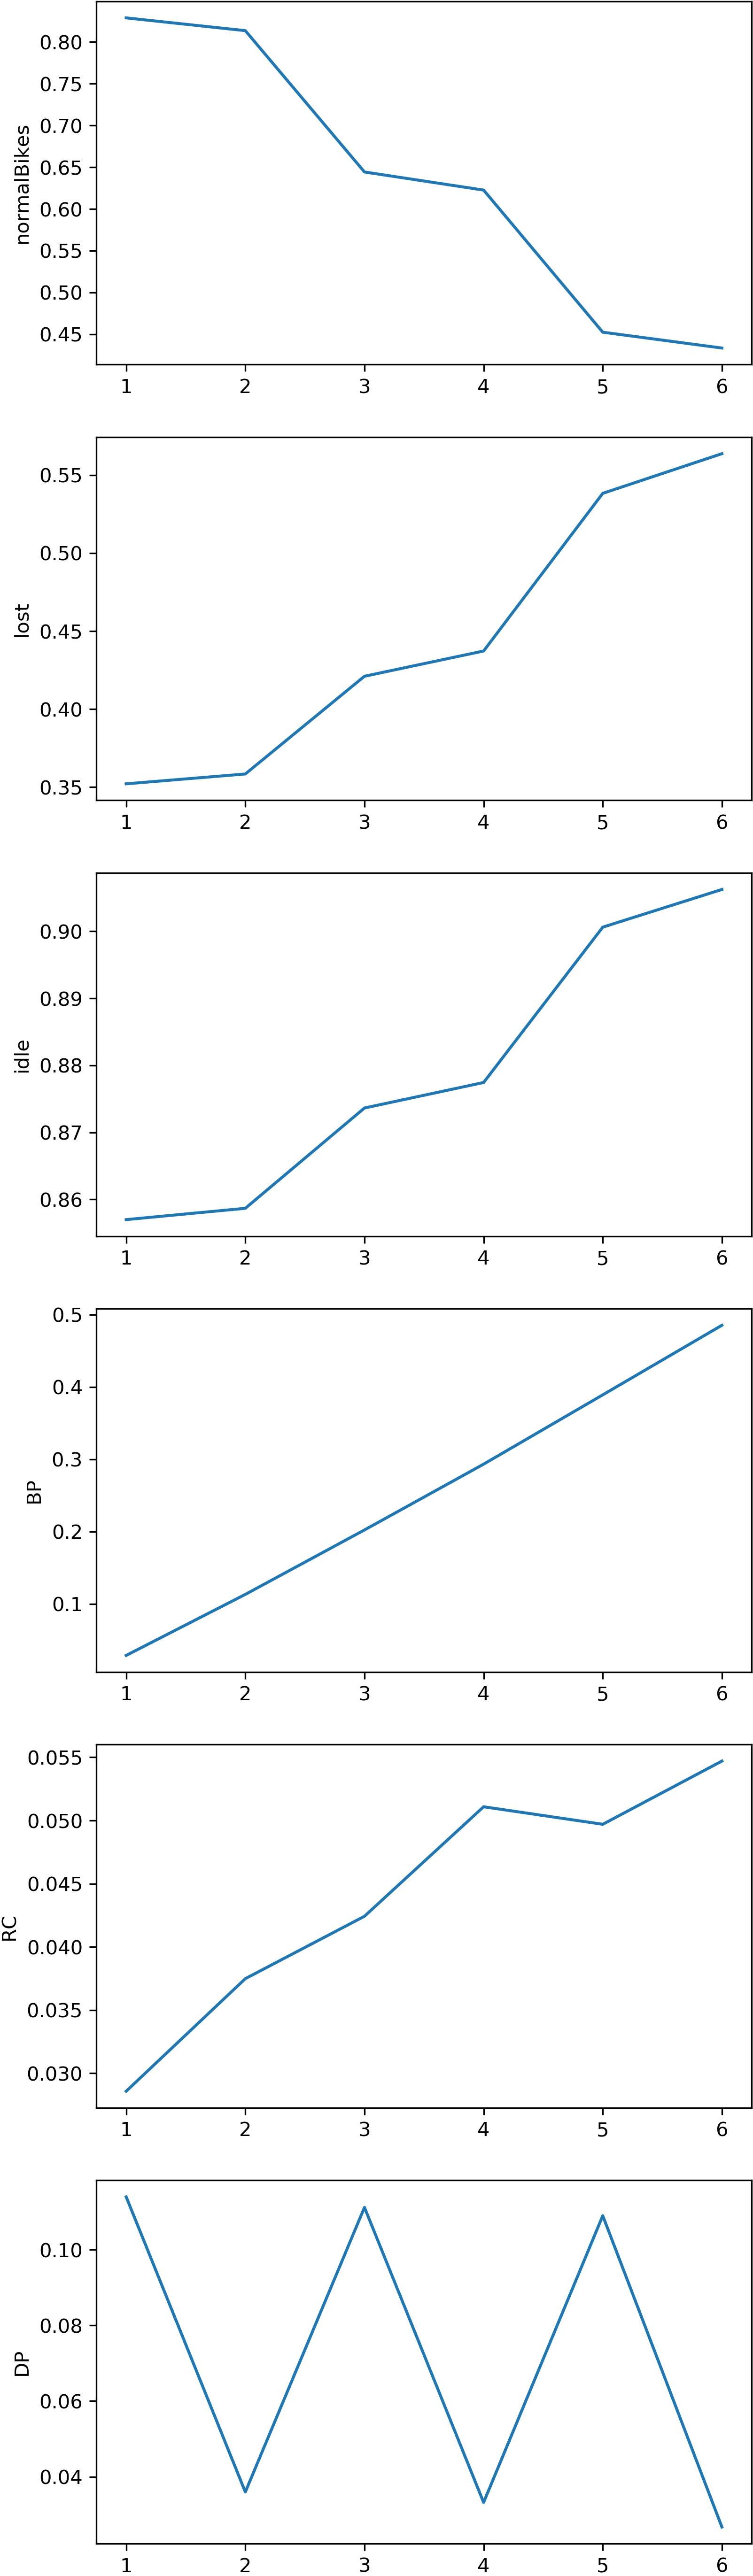
\includegraphics[width=2.3in]{Graph/perfB_1-6.png}
%     %\caption{fig2}
%     \end{minipage}%
%     }%
% \end{figure}
% \restoregeometry

% \newgeometry{left=0.1cm,right=0.1cm, top=0.1cm, bottom=0.1cm}
% \begin{figure}[h]
%     \centering
%     \subfigure[Mu]{
%     \begin{minipage}[t]{0.5\linewidth}
%     \centering
%     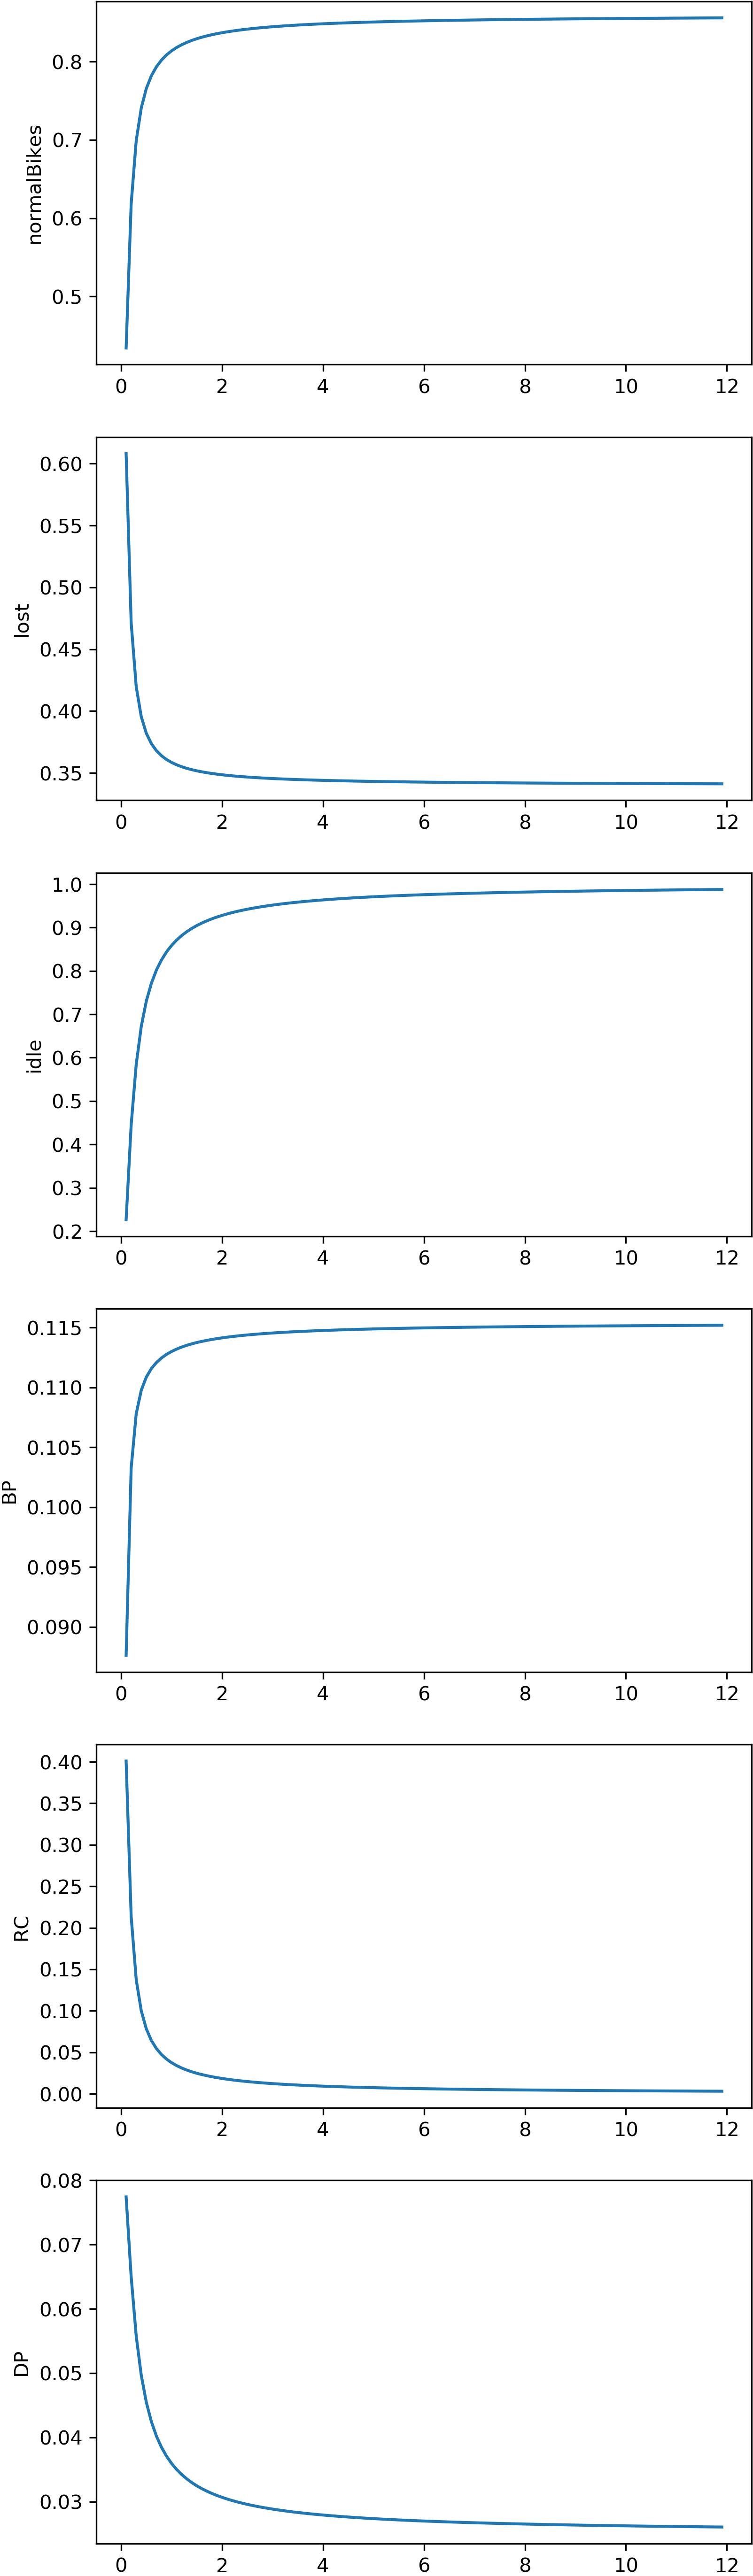
\includegraphics[width=2.3in]{Graph/perfMu0-12.png}
%     %\caption{fig1}
%     \end{minipage}%
%     }%
%     \centering
%     \subfigure[N]{
%     \begin{minipage}[t]{0.5\linewidth}
%     \centering
%     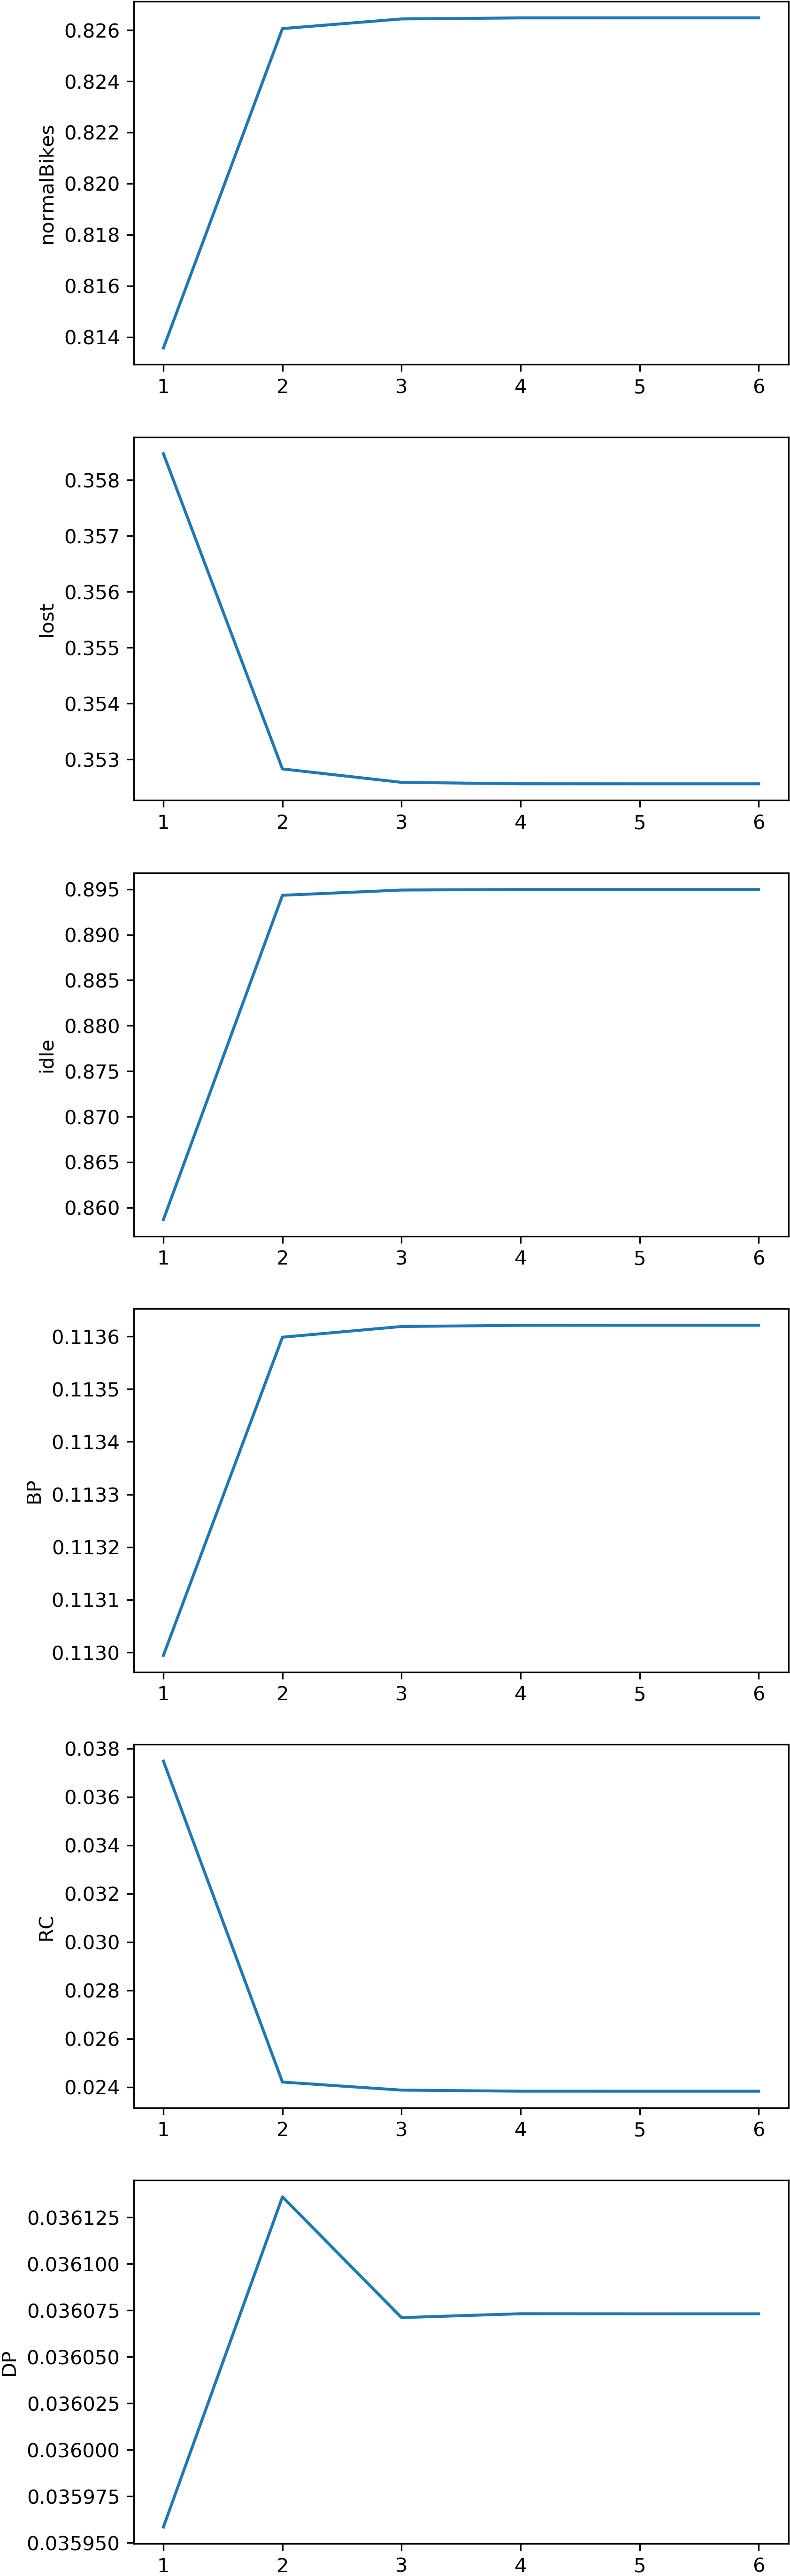
\includegraphics[width=2.3in]{Graph/perfN1-6.png}
%     %\caption{fig2}
%     \end{minipage}%
%     }%
% \end{figure}
% \restoregeometry

% \newgeometry{left=0.1cm,right=0.1cm, top=0.1cm, bottom=0.1cm}
% \begin{figure}[h]
%     \centering
%     \subfigure[Delta]{
%     \begin{minipage}[t]{0.5\linewidth}
%     \centering
%     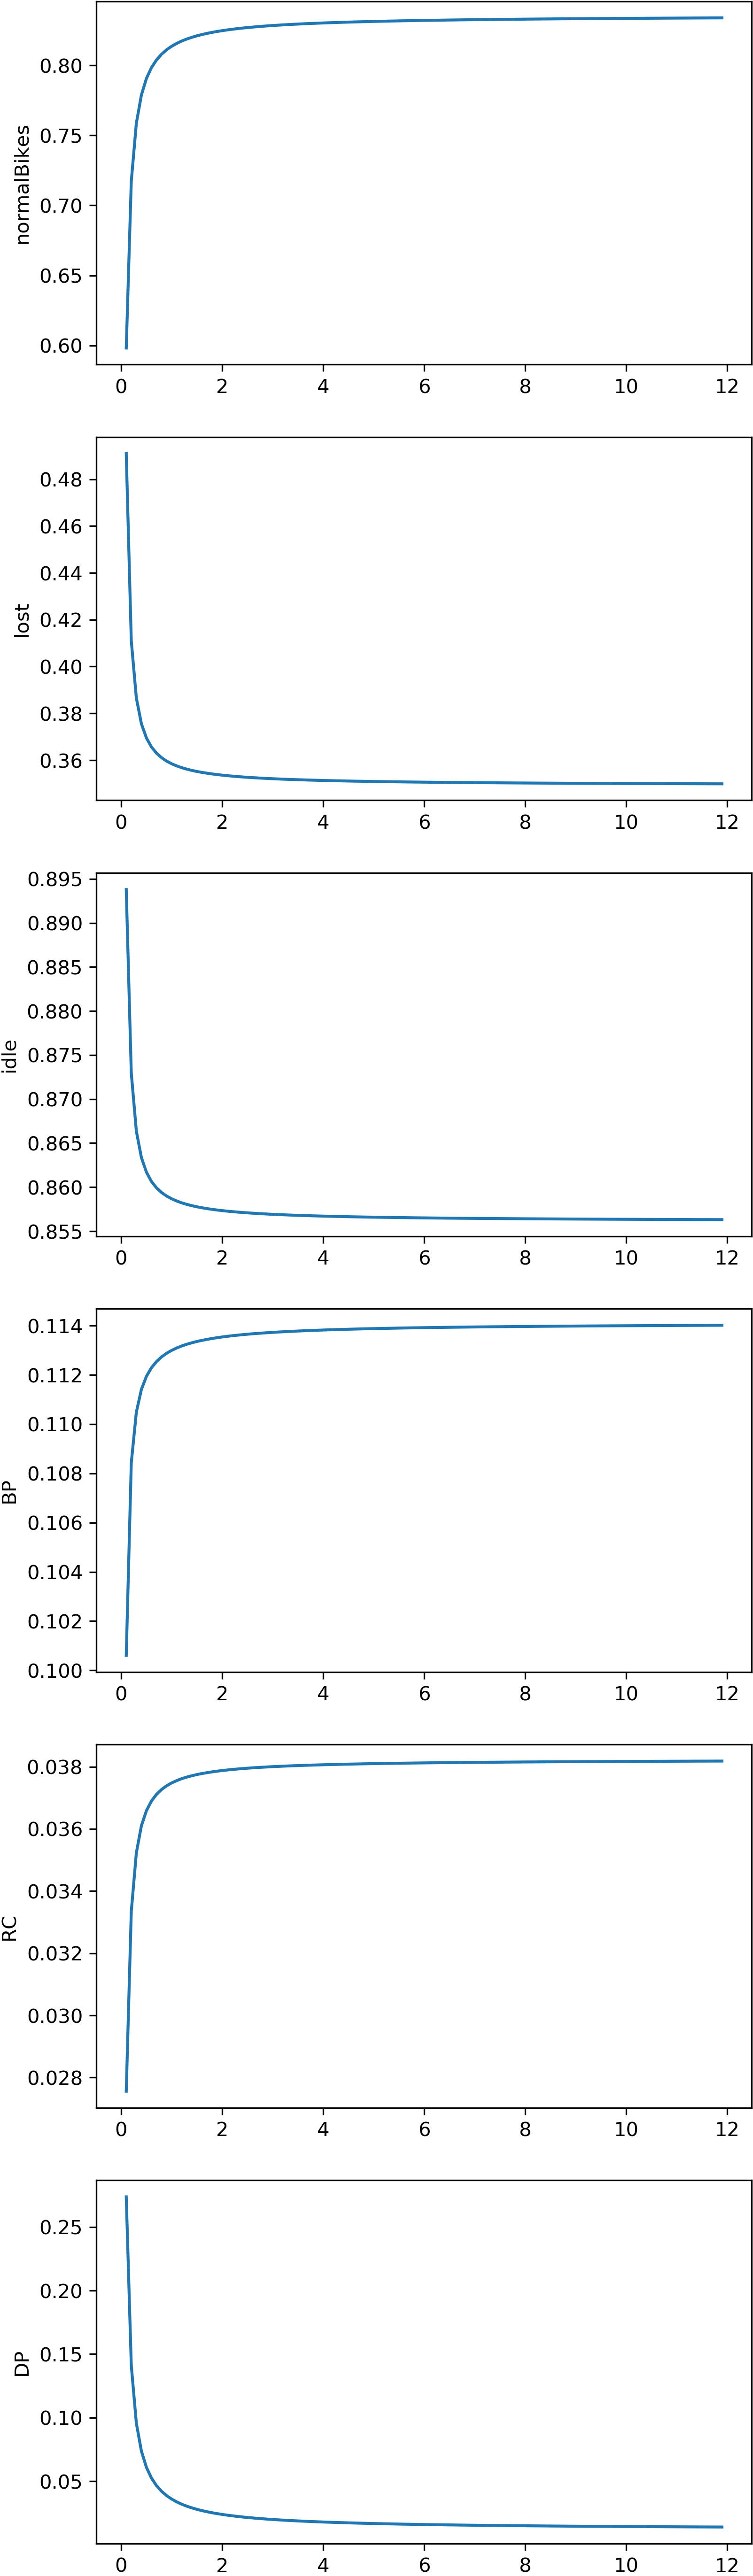
\includegraphics[width=2.3in]{Graph/perfDelta0-12.png}
%     %\caption{fig1}
%     \end{minipage}%
%     }%
%     \centering
%     \subfigure[$\overline{D}$]{
%     \begin{minipage}[t]{0.5\linewidth}
%     \centering
%     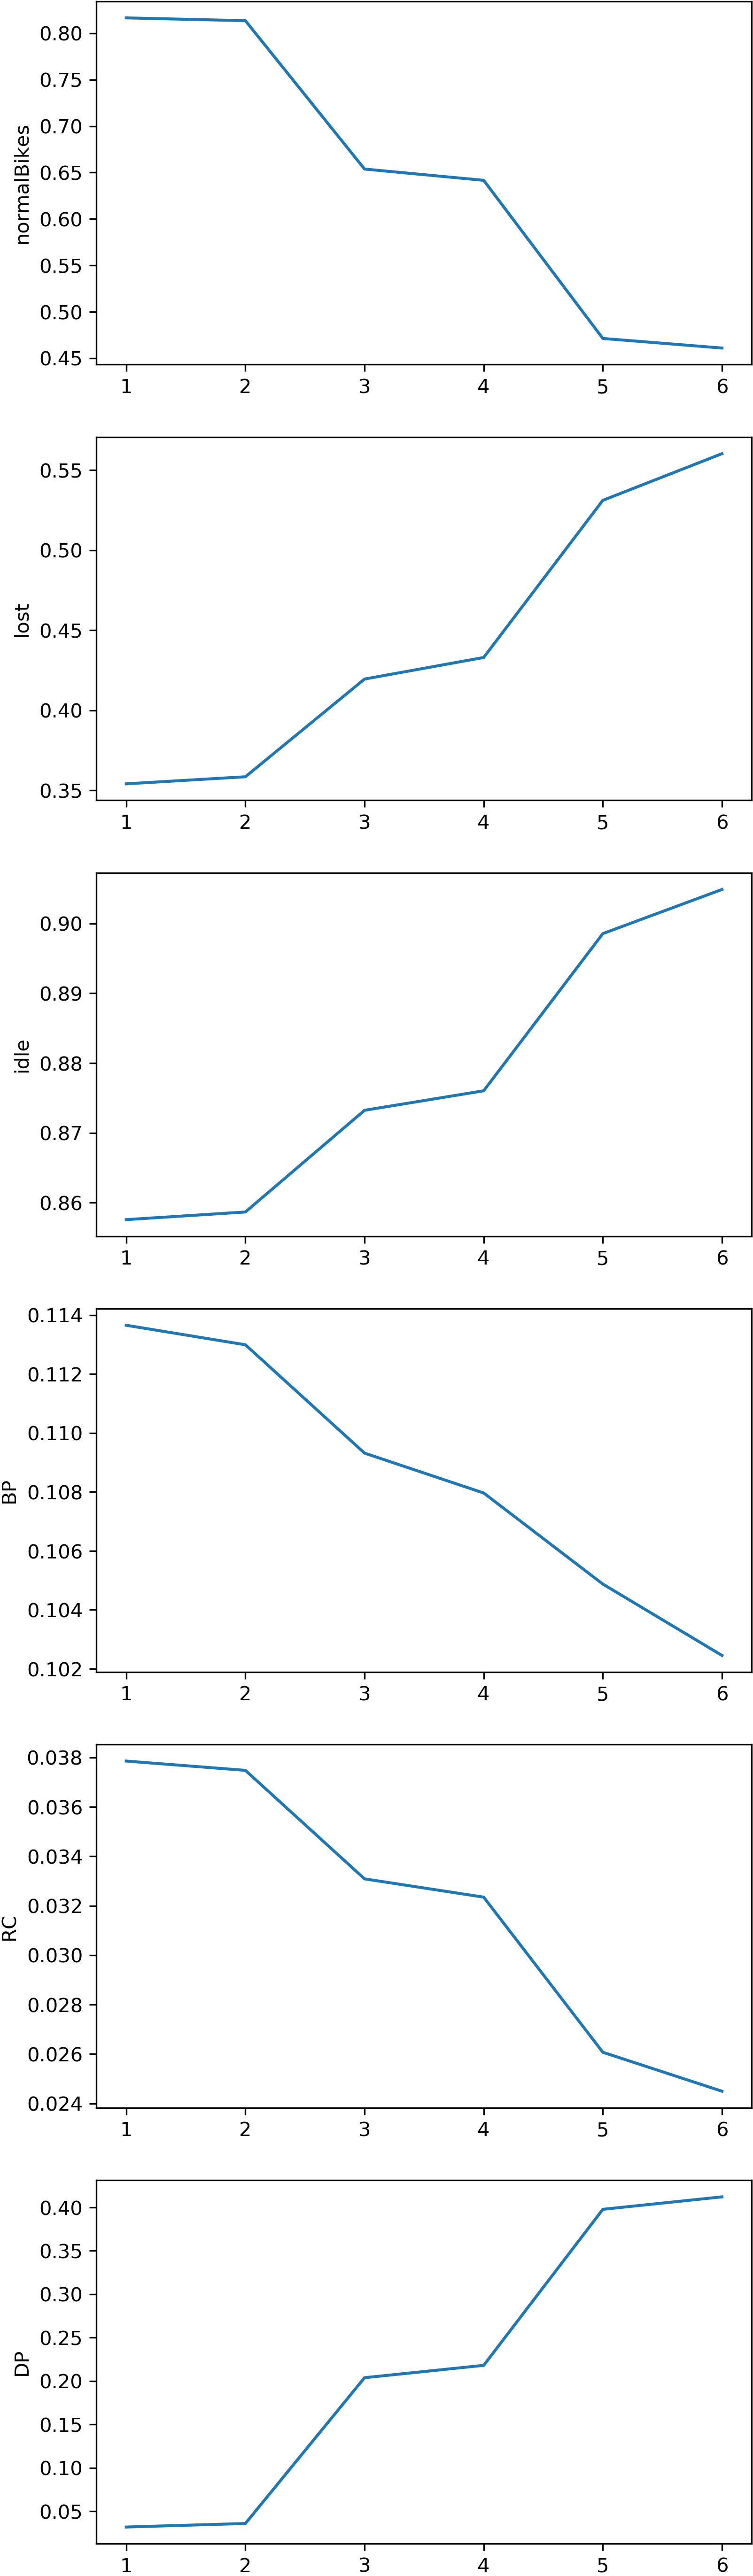
\includegraphics[width=2.3in]{Graph/perfD_1-6.png}
%     %\caption{fig2}
%     \end{minipage}%
%     }%
% \end{figure}
% \restoregeometry